\documentclass[12pt]{article}
\usepackage[english]{babel}
\usepackage{natbib}
\usepackage{pdfpages}
\usepackage{float}
\usepackage{url}
\usepackage[utf8x]{inputenc}
\usepackage{amsmath}
\usepackage{graphicx}
\graphicspath{{images/}}
\usepackage{parskip}
\usepackage{fancyhdr}
% \usepackage{vmargin}
% \setmarginsrb{2 cm}{2.5 cm}{2 cm}{2.5 cm}{1 cm}{1.5 cm}{1 cm}{1.5 cm}
\usepackage[a4paper,left=2.5cm,right=3cm]{geometry}
\addtolength{\topmargin}{-0.5cm}
% \setmarginsrb{3 cm}{2.5 cm}{3 cm}{2.5 cm}{1 cm}{1.5 cm}{1 cm}{1.5 cm}

\title{Workshop on Spoken Dialogue Systems for PhDs, PostDocs and New Researchers}								% Title
% \author{Chong Hui Yong}								% Author
\date{September 16, 2016}											% Date

\def\EDITION{{12}}  % 12 was for 2016 workshop

\newcommand\textbox[1]{%
      \parbox{.333\textwidth}{#1}%
}

\makeatletter
\let\thetitle\@title
% \let\theauthor\@author
\let\thedate\@date
\makeatother

\pagestyle{fancy}
\fancyhf{}
\lhead{\thetitle}
\cfoot{\thepage}

\begin{document}

%%%%%%%%%%%%%%%%%%%%%%%%%%%%%%%%%%%%%%%%%%%%%%%%%%%%%%%%%%%%%%%%%%%%%%%%%%%%%%%%%%%%%%%%%

\begin{titlepage}
	\centering
    \vspace*{0.1 cm}
    
\includegraphics[scale = 0.8]{yrrsds_logo.png}\\[1.0 cm]
    \textsc{\LARGE ICT, Los Angeles, USA}\\[2.0 cm]
	\textsc{\Large Proceedings 2016}\\[0.5 cm]
	\rule{\linewidth}{0.2 mm} \\[0.4 cm]
	{ \huge \bfseries \thetitle}\\
	\rule{\linewidth}{0.2 mm} \\[1.0 cm]
	
\begin{figure}[H]
\centering
    % TODO sponsors
    
\includegraphics[scale=0.4]{yrrsds_logo.png} \\
\end{figure}
	
	{\large \thedate}\\[2 cm]
\end{titlepage}


\section*{Foreword}
The Young Researchers Roundtable on Spoken Dialog Systems (YRRSDS) has been for many of us our first encounter with life in the research world. It aspires to be an environment in which young researchers can present late-breaking work, discuss ideas, connect with other researchers, and hear first person accounts of what it means to be a part of this field straight from respected senior members in the industry and academy.

There is an additional angle that is often overlooked, which is that YRRSDS is also the perfect stepping stone for anyone newly entering this field. Before the “big league” conferences, YRRSDS serves as an ideal forum for young researchers to discuss ideas in a laid-back setting with others who may have as many doubts and questions. This circulation of fresh perspectives has the potential for great impact on the next generation of research. The Roundtable’s focus has always been to foster creative thinking and strengthen an international network of researchers. Past, present, and future YRRSDS participants form a pipeline of mentors and colleagues as former YRRSDS become senior professionals themselves. We are proud to be part of the chain of young researchers carrying these ideals into the present day.

We hope you enjoy the Roundtable. It’s been a privilege for us to host its \EDITION th edition, and it’s our honor to have you join us. If you take away from YRRSDS as much as we have, we encourage you to volunteer for organizing next year’s YRRSDS to keep the torch moving towards the future.

\hfill {\bf The YRRSDS \the\year \ committee}
\pagebreak

\section*{Organizing Committee}

\begin{itemize}
\item Alexandros Papangelis, Toshiba CRL
\item David Cohen, Carnegie Mellon University
\item Eli Pincus, University of Southern California
\item José David Lopes, KTH Royal Institute of Technology
\item Ondřej Plátek, Charles University in Prague
\item Lu Chen, Shanghai Jiao Tong University
\item Maria Schmidt, KIT Karlsruhe Institute of Technology
\item Ramesh Manuvinakurike, University of Southern California
\item Tiancheng Zhao, Carnegie Mellon University
\item Zhou Yu, Carnegie Mellon University
\end{itemize}

\section*{Advisory Committee}

\begin{itemize}
\item Srinivas Bangalore, Interactions (former AT\&T Research)
\item Luciana Benotti, Universidad Nacional de Córdoba
\item Rolf Carlson, KTH Royal Institute of Technology
\item Maxine Eskenazi, Carnegie Mellon University
\item Kallirroi Georgila, University of Southern California
\item Jim Glass, Massachusetts Institute of Technology
\item Kristiina Jokinen, University of Helsinki
\item Tatsuya Kawahara, Kyoto University
\item Diane Litman, University of Pittsburgh
\item Wolfgang Minker, University of Ulm
\item Sebastian Möller, Technische Universität Berlin
\item Mikio Nakano, Honda Research Institute
\item David Schlangen, Universität Bielefeld
\item Gabriel Skantze, KTH Royal Institute of Technology
\item David Traum, University of Southern California
\item Nigel Ward, University of Texas at El Paso
\item Jason Williams, Microsoft Research
\item Steve Young, University of Cambridge
\item Oliver Lemon, Heriot-Watt University
\item Alex Lascarides, University of Edinburgh
\item Sungjin Lee, Yahoo!
\item Timothy Bickmore, Northeastern University
\item L P Morency, Carnegie Mellon University
\item David DeVault, USC Institute for Creative technologies
\item Matthew Purver, Queen Mary University, London
\item Julia Hirschberg, Columbia University
\item Deepak Ramachandran, Nuance Communications
\item Svetlana Stoyanchev, Interactions Corporations 
\end{itemize}
\pagebreak

%%%%%%%%%%%%%%%%%%%%%%%%%%%%%%%%%%%%%%%%%%%%%%%%%%%%%%%%%%%%%%%%%%%%%%%%%%%%%%%%%%%%%%%%%

\tableofcontents
\pagebreak

%%%%%%%%%%%%%%%%%%%%%%%%%%%%%%%%%%%%%%%%%%%%%%%%%%%%%%%%%%%%%%%%%%%%%%%%%%%%%%%%%%%%%%%%%

\section{Invited talks}
\subsection{Natural Language Generation for Dialogue Systems: What we (still) don't know. Marilyn Walker, UC Santa Cruz}
Abstract:  Dialogue interaction provides an extremely challenging and grounded evaluation of natural language understanding. Natural language understanding has greatly improved over the last 20 years, but what level of understanding is needed to respond appropriately in dialogue in a particular context? How can natural language generation produce these contextually appropriate responses? How can it scale? Should a conversational assistant have a persona or style? Should it entrain to the user, take the initiative, understand greetings and other phatic acts, and use an explicit model of dialogue structure? What are some near term and some
long term solutions towards more natural dialogue interaction?

\subsection{Stefan Scherer (USC ICT)}
\subsection{Gokhan Tur (Google Research)}

\section{Notes from discussions}
Discussions are core of the workshop and the reason to organize it. 
The notes taken by organizers is a subjective attempt to capture some conclusions.

\subsection{Building Chatbots}
to apear
\subsection{Commercial SDSs}
to apear
\subsection{Evaluating Chatbots}
to apear
\subsection{Multi-Modal Understanding}
to apear
\subsection{Multi-Modal Generation}
to appear
\subsection{Advances in Statistical Methods for SDSs}
to appear
\subsection{Learning Through Interaction}
to appear
\subsection{Multi-Domain DM}
to appear
\subsection{Long Term Interaction}
to appear
\subsection{Crowd and Simulated Evaluation of Dialog Systems}
to appear
 

\section{Position papers}


% 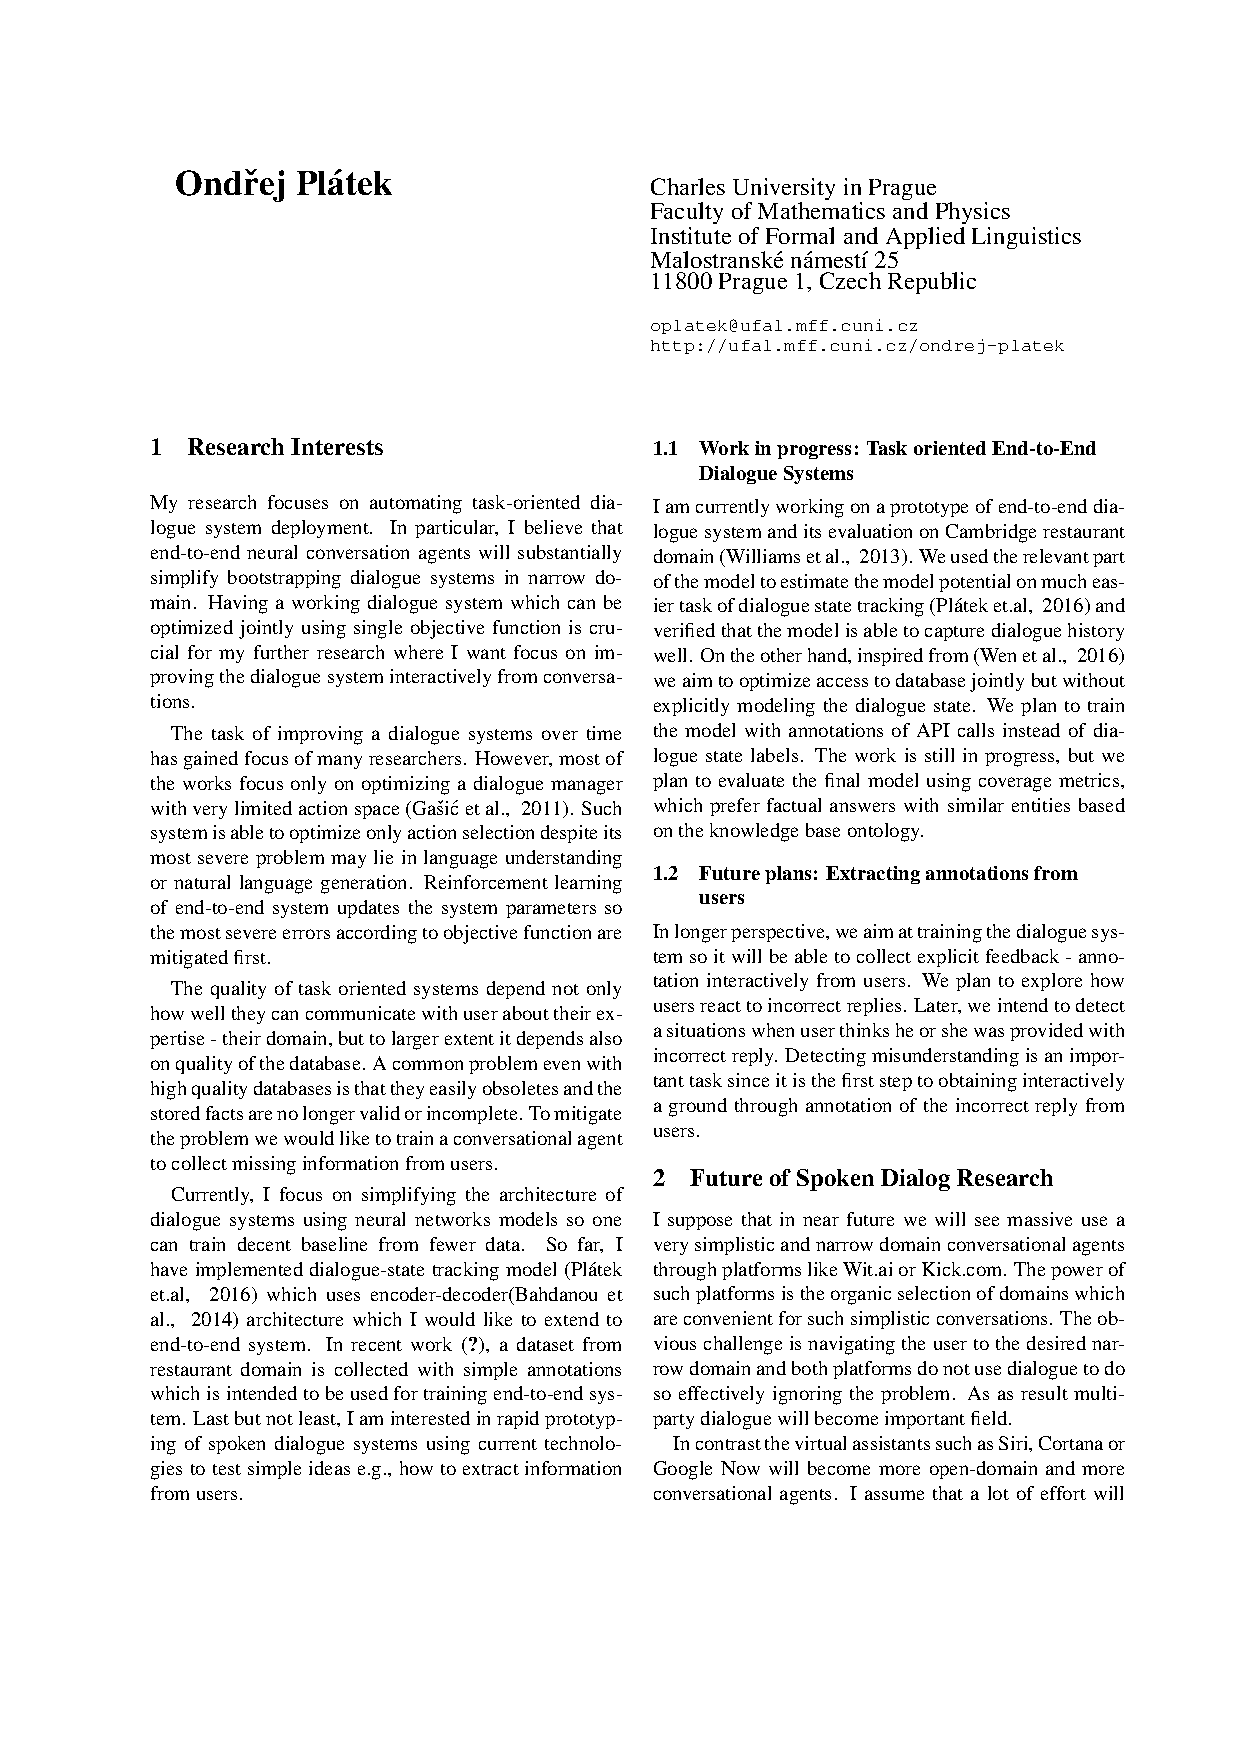
\includepdf[pages=-,pagecommand={},width=\textwidth]{YRRSDS_2016_paper_1_ondrej_platek.pdf}
% 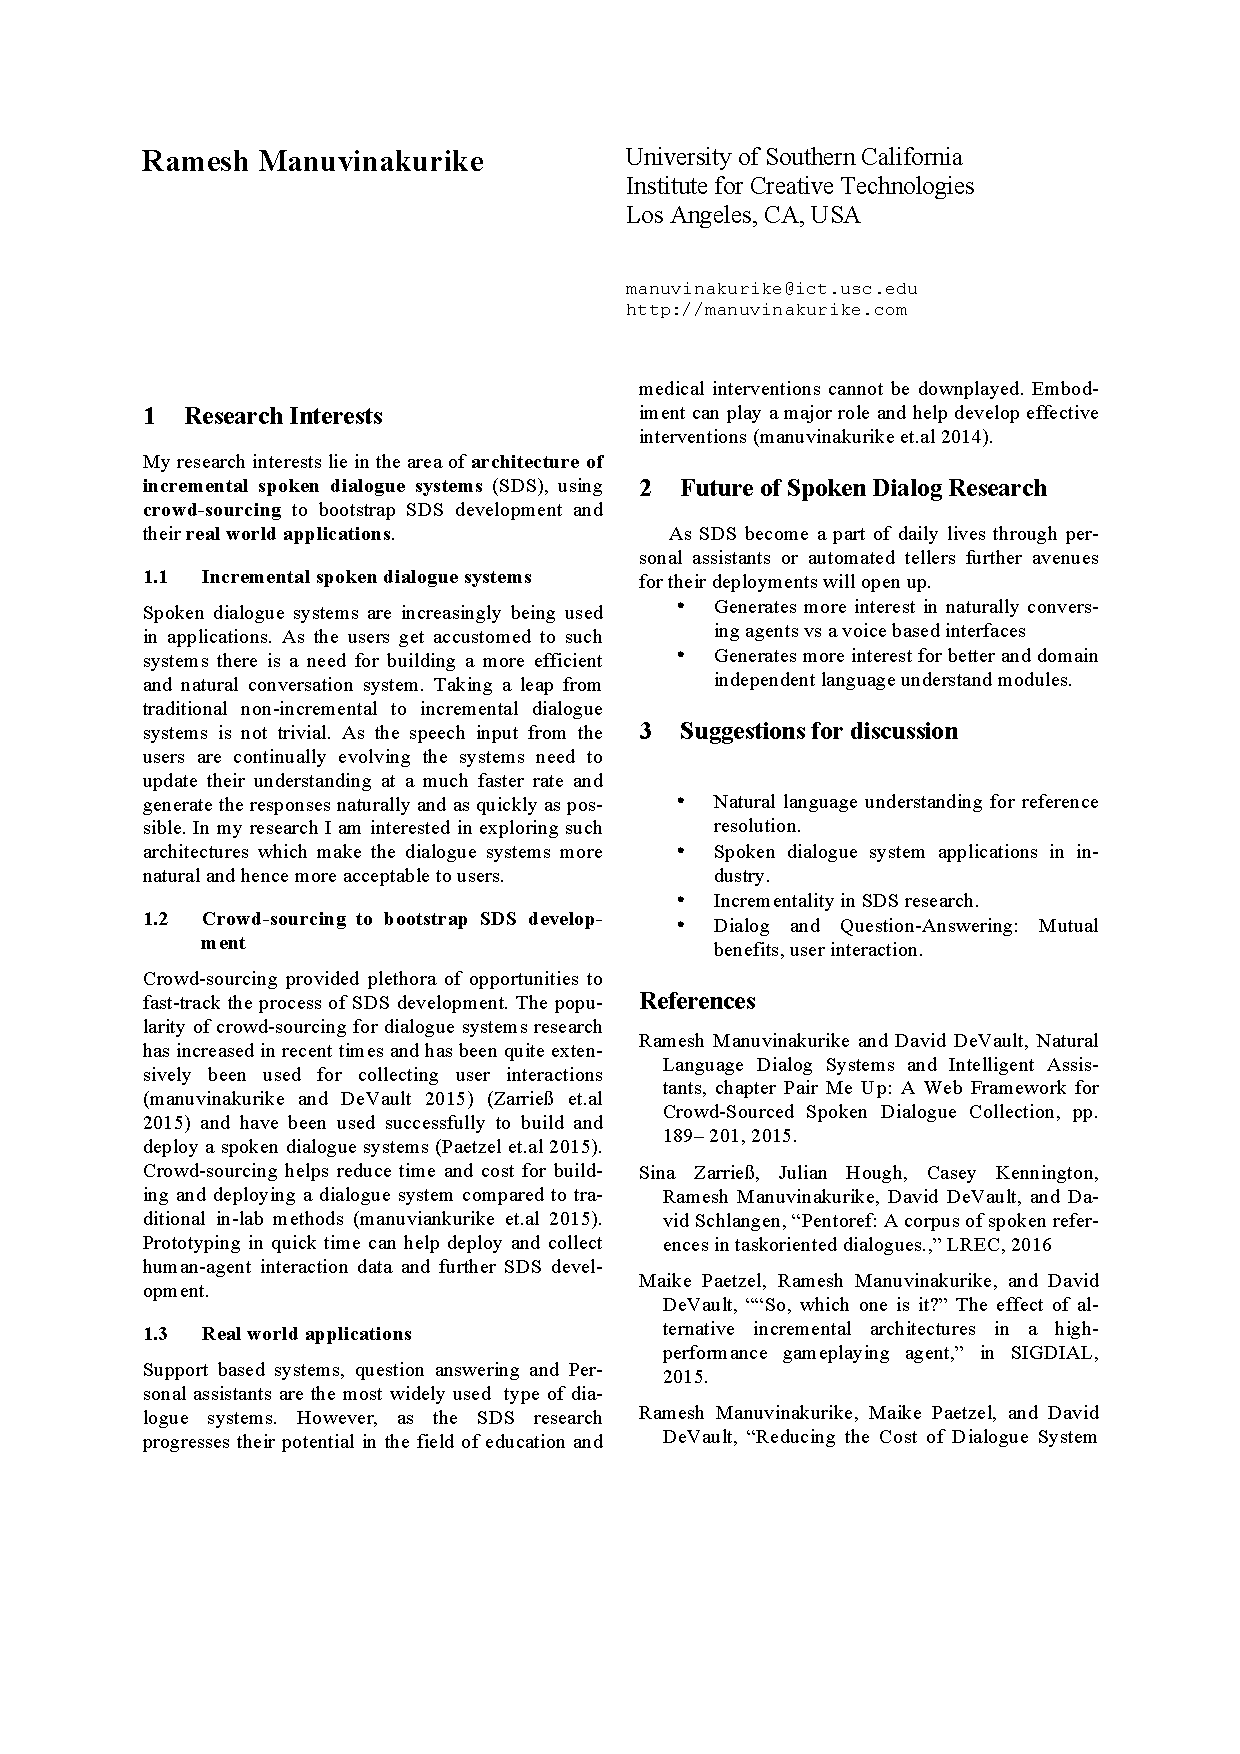
\includepdf[pages=-,pagecommand={},width=\textwidth]{YRRSDS_2016_paper_2_remesh_manuvinakurike.pdf}
% 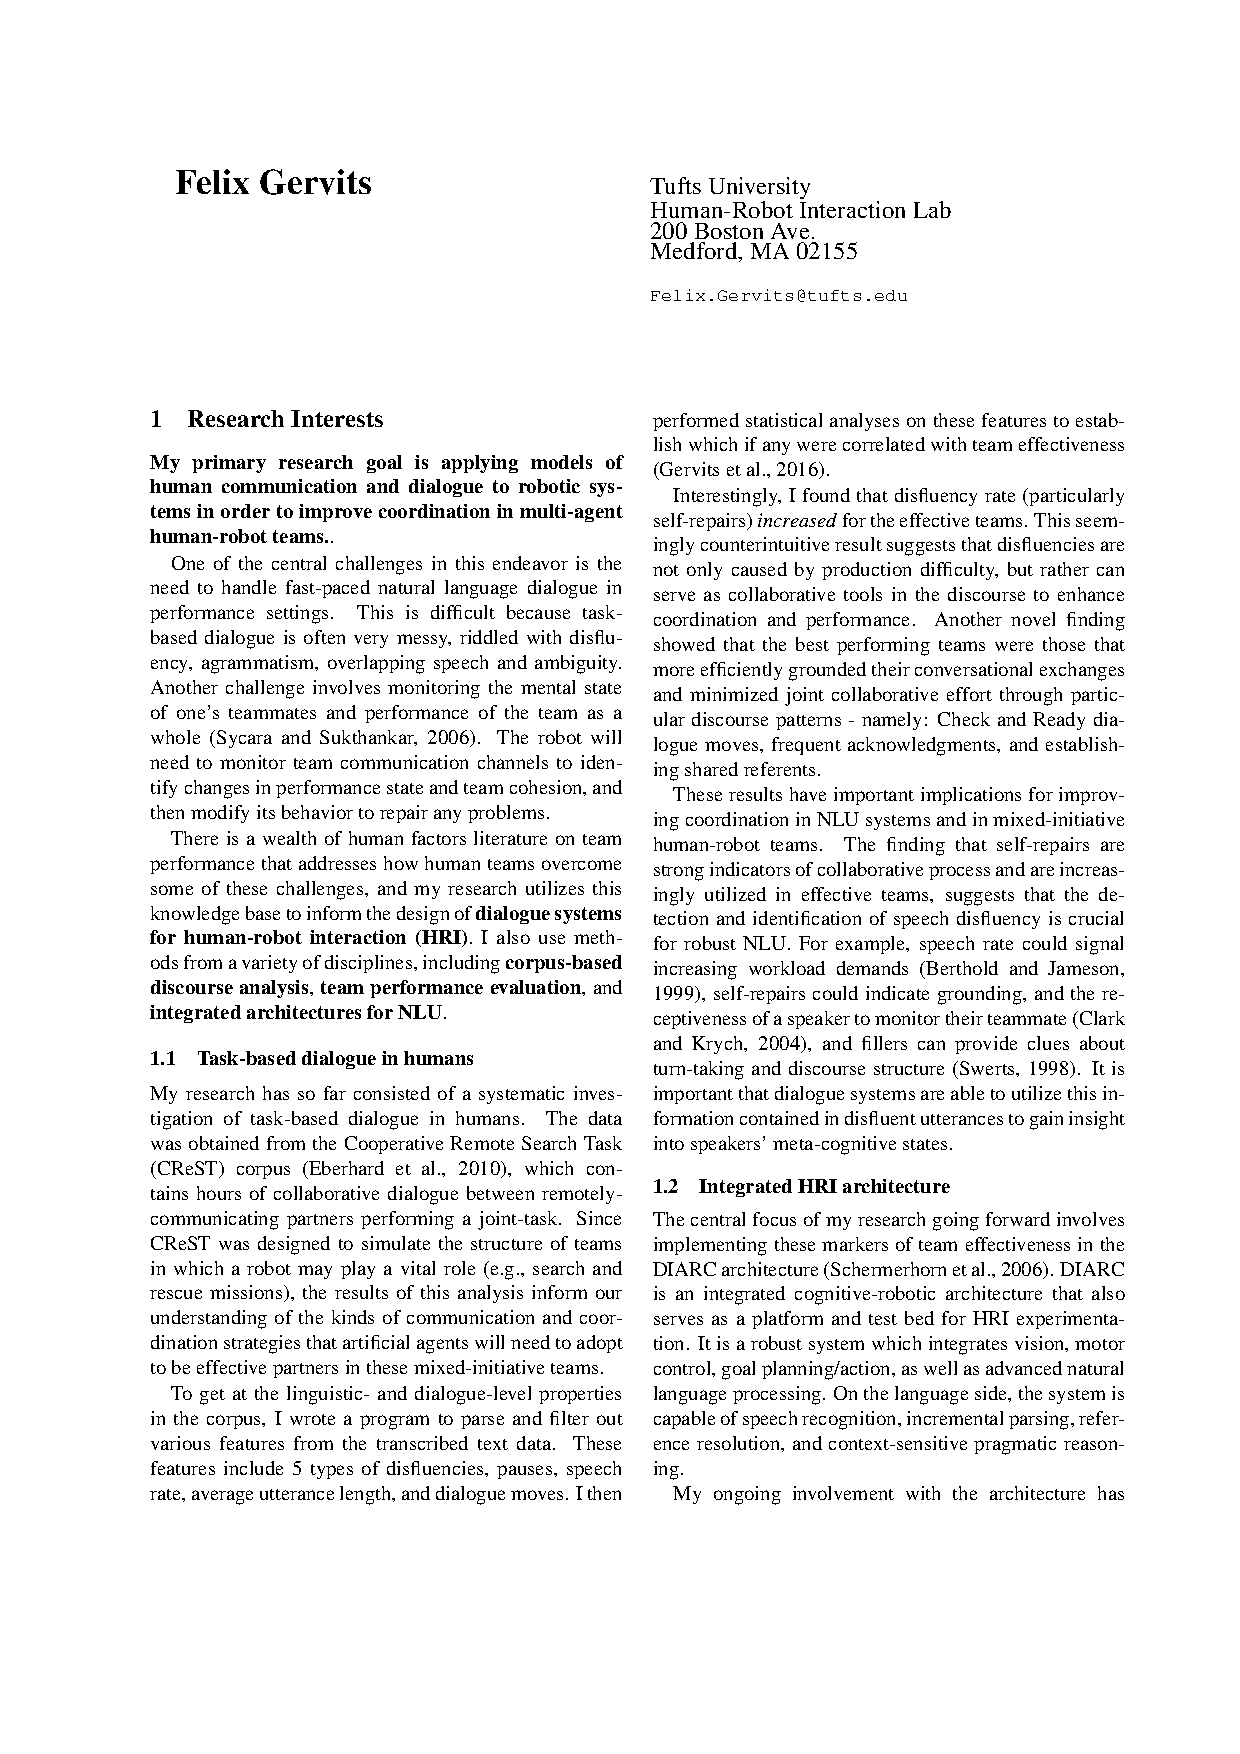
\includepdf[pages=-,pagecommand={},width=\textwidth]{YRRSDS_2016_paper_3_felix_gervits.pdf}
% 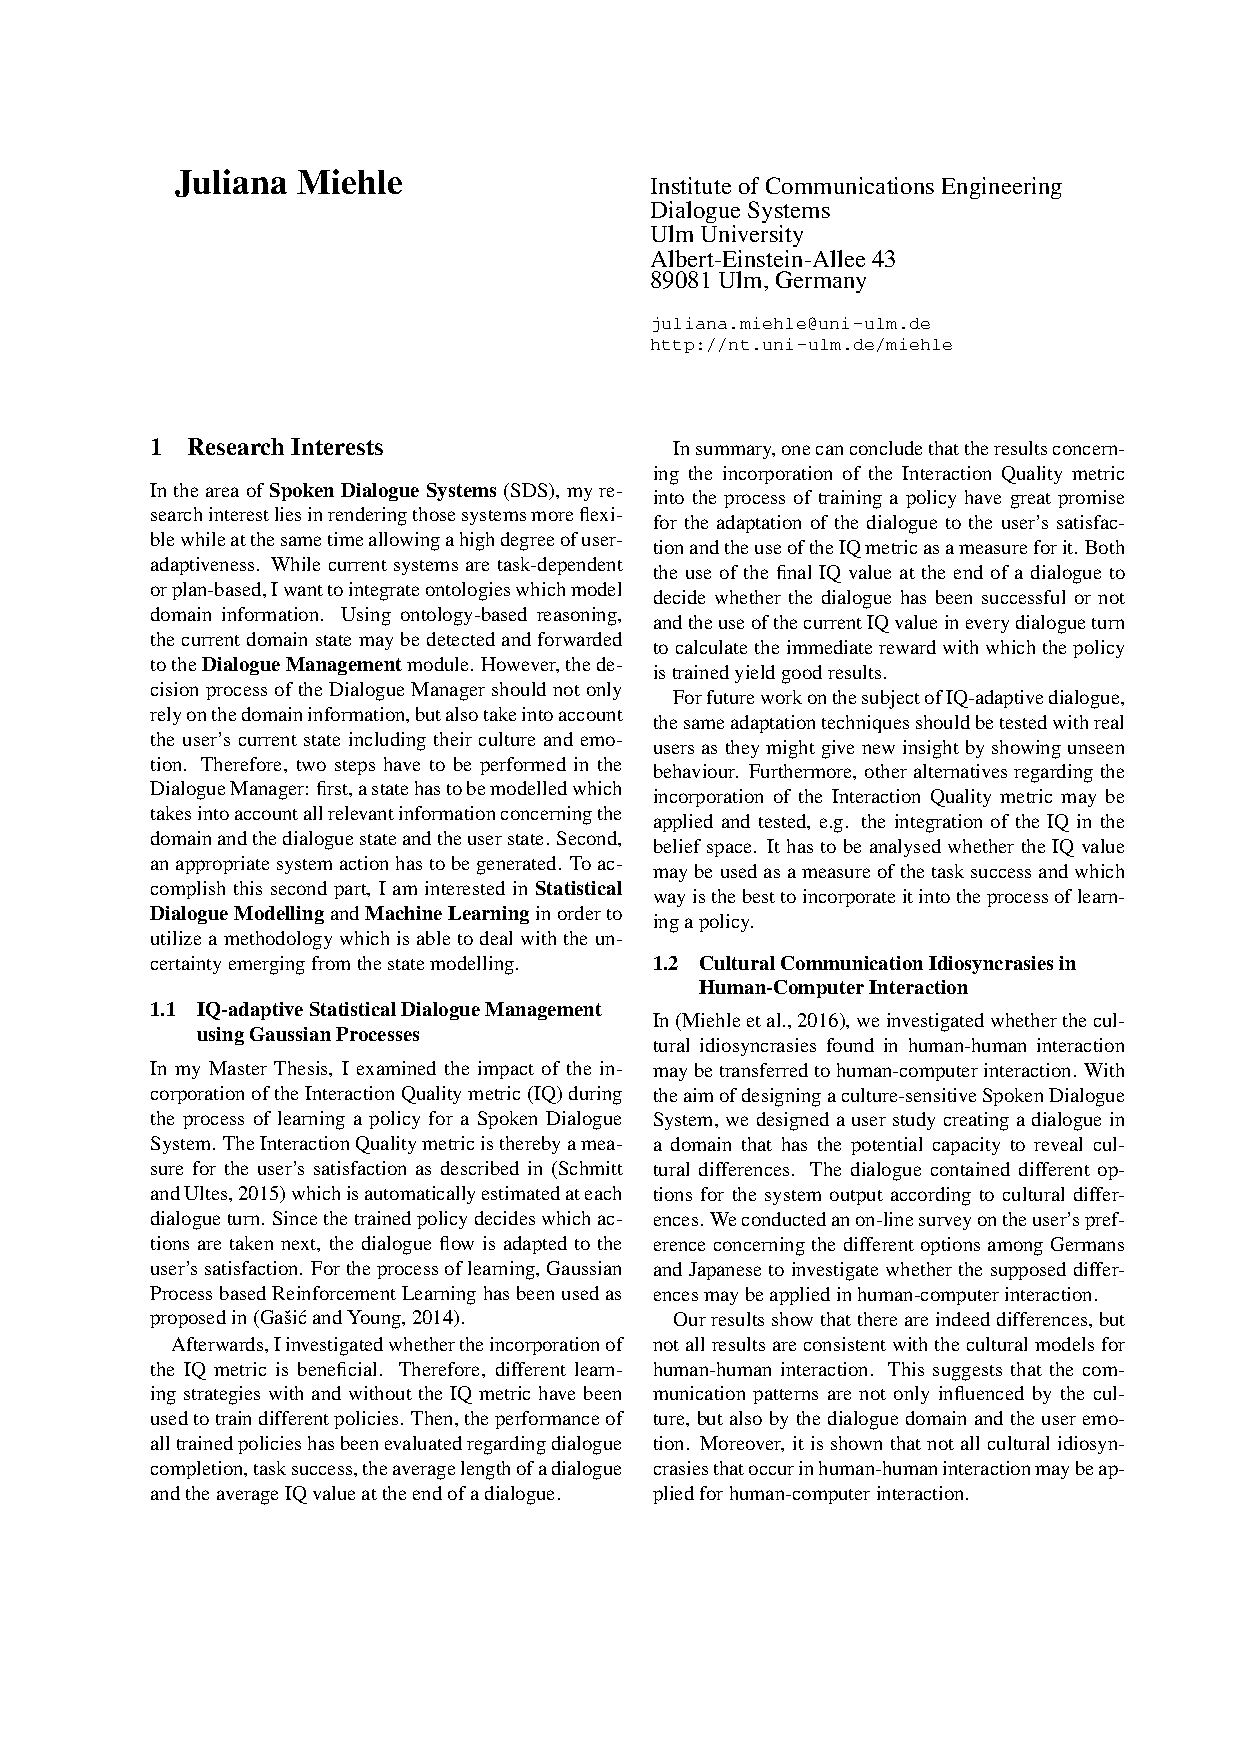
\includepdf[pages=-,pagecommand={},width=\textwidth]{YRRSDS_2016_paper_4_juliana_miehle.pdf}
% 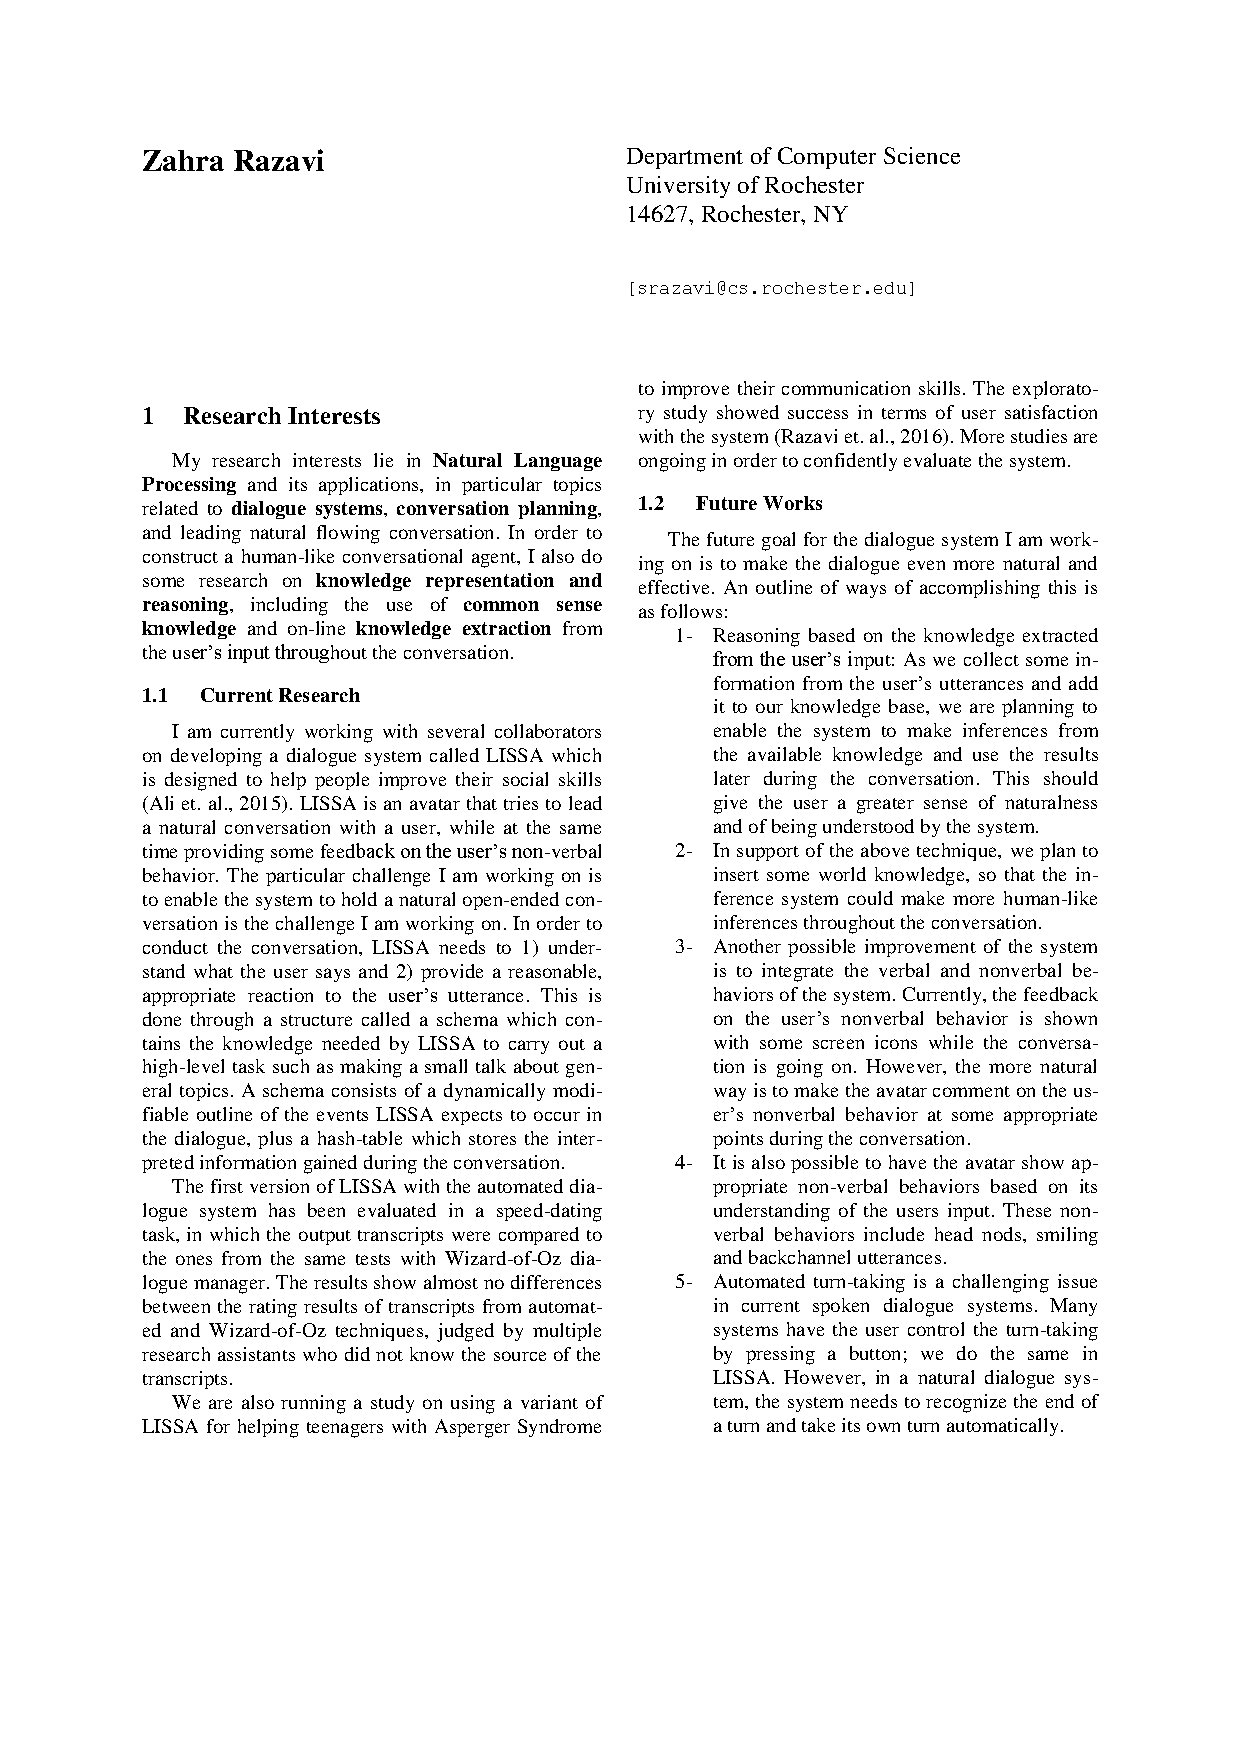
\includepdf[pages=-,pagecommand={},width=\textwidth]{YRRSDS_2016_paper_5_zahra_razavi.pdf}
% 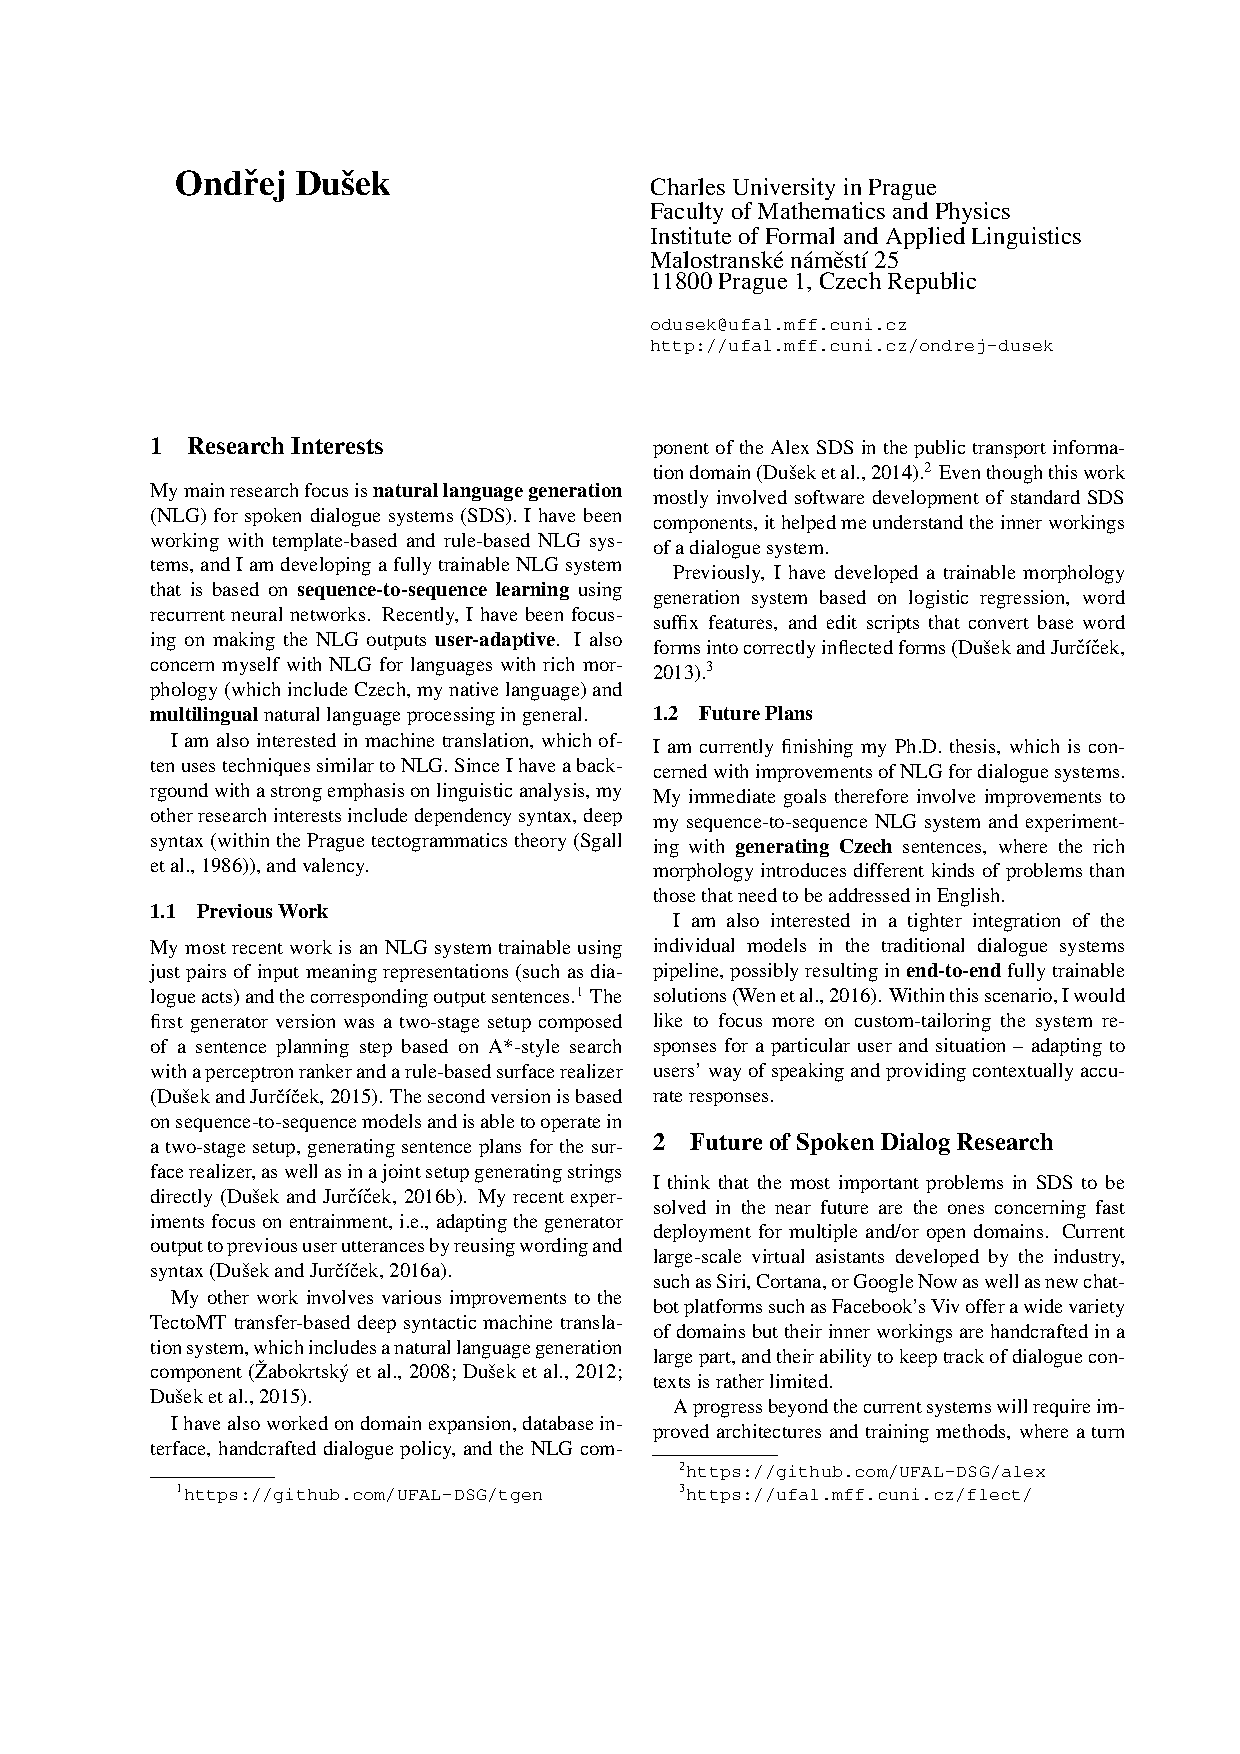
\includepdf[pages=-,pagecommand={},width=\textwidth]{YRRSDS_2016_paper_6_ondrej_dusek.pdf}
% 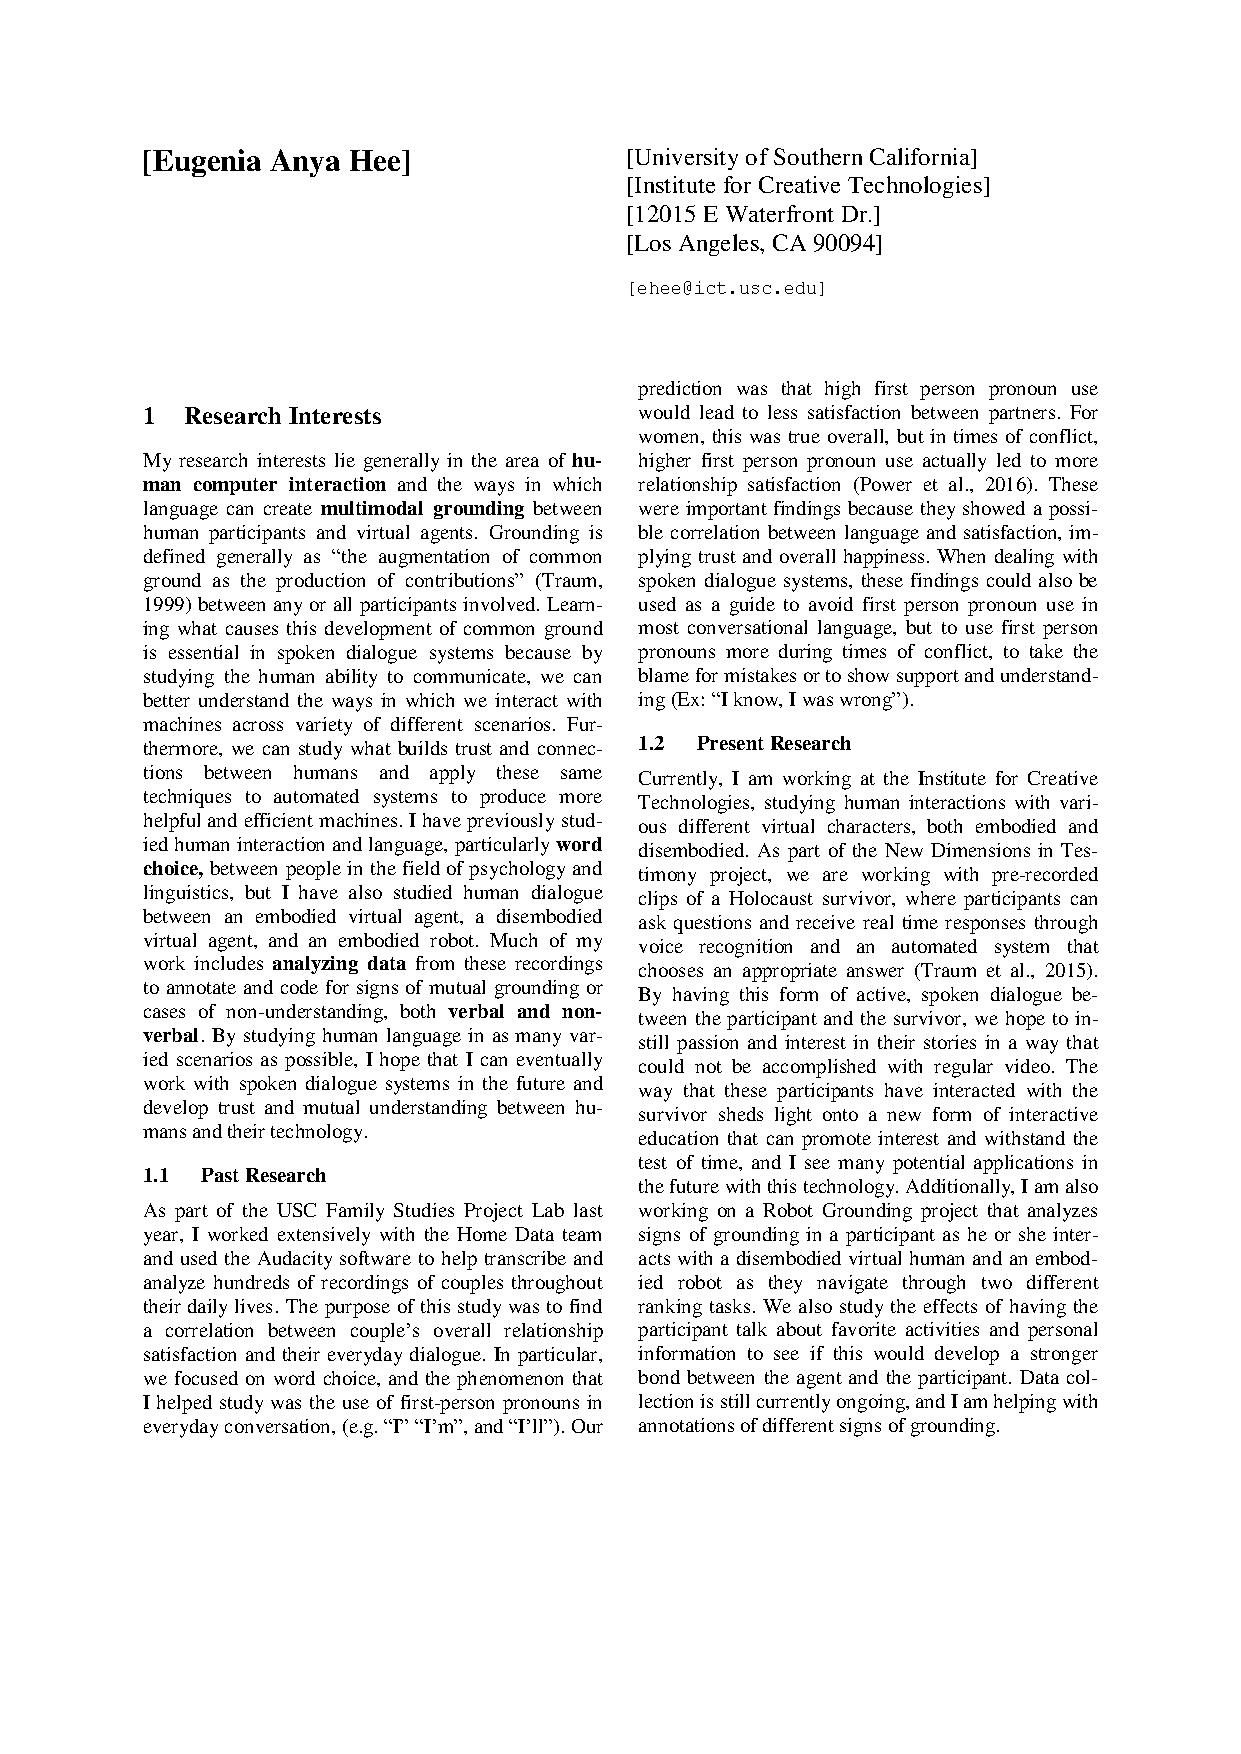
\includepdf[pages=-,pagecommand={},width=\textwidth]{YRRSDS_2016_paper_7_eugenia_hee.pdf}
% 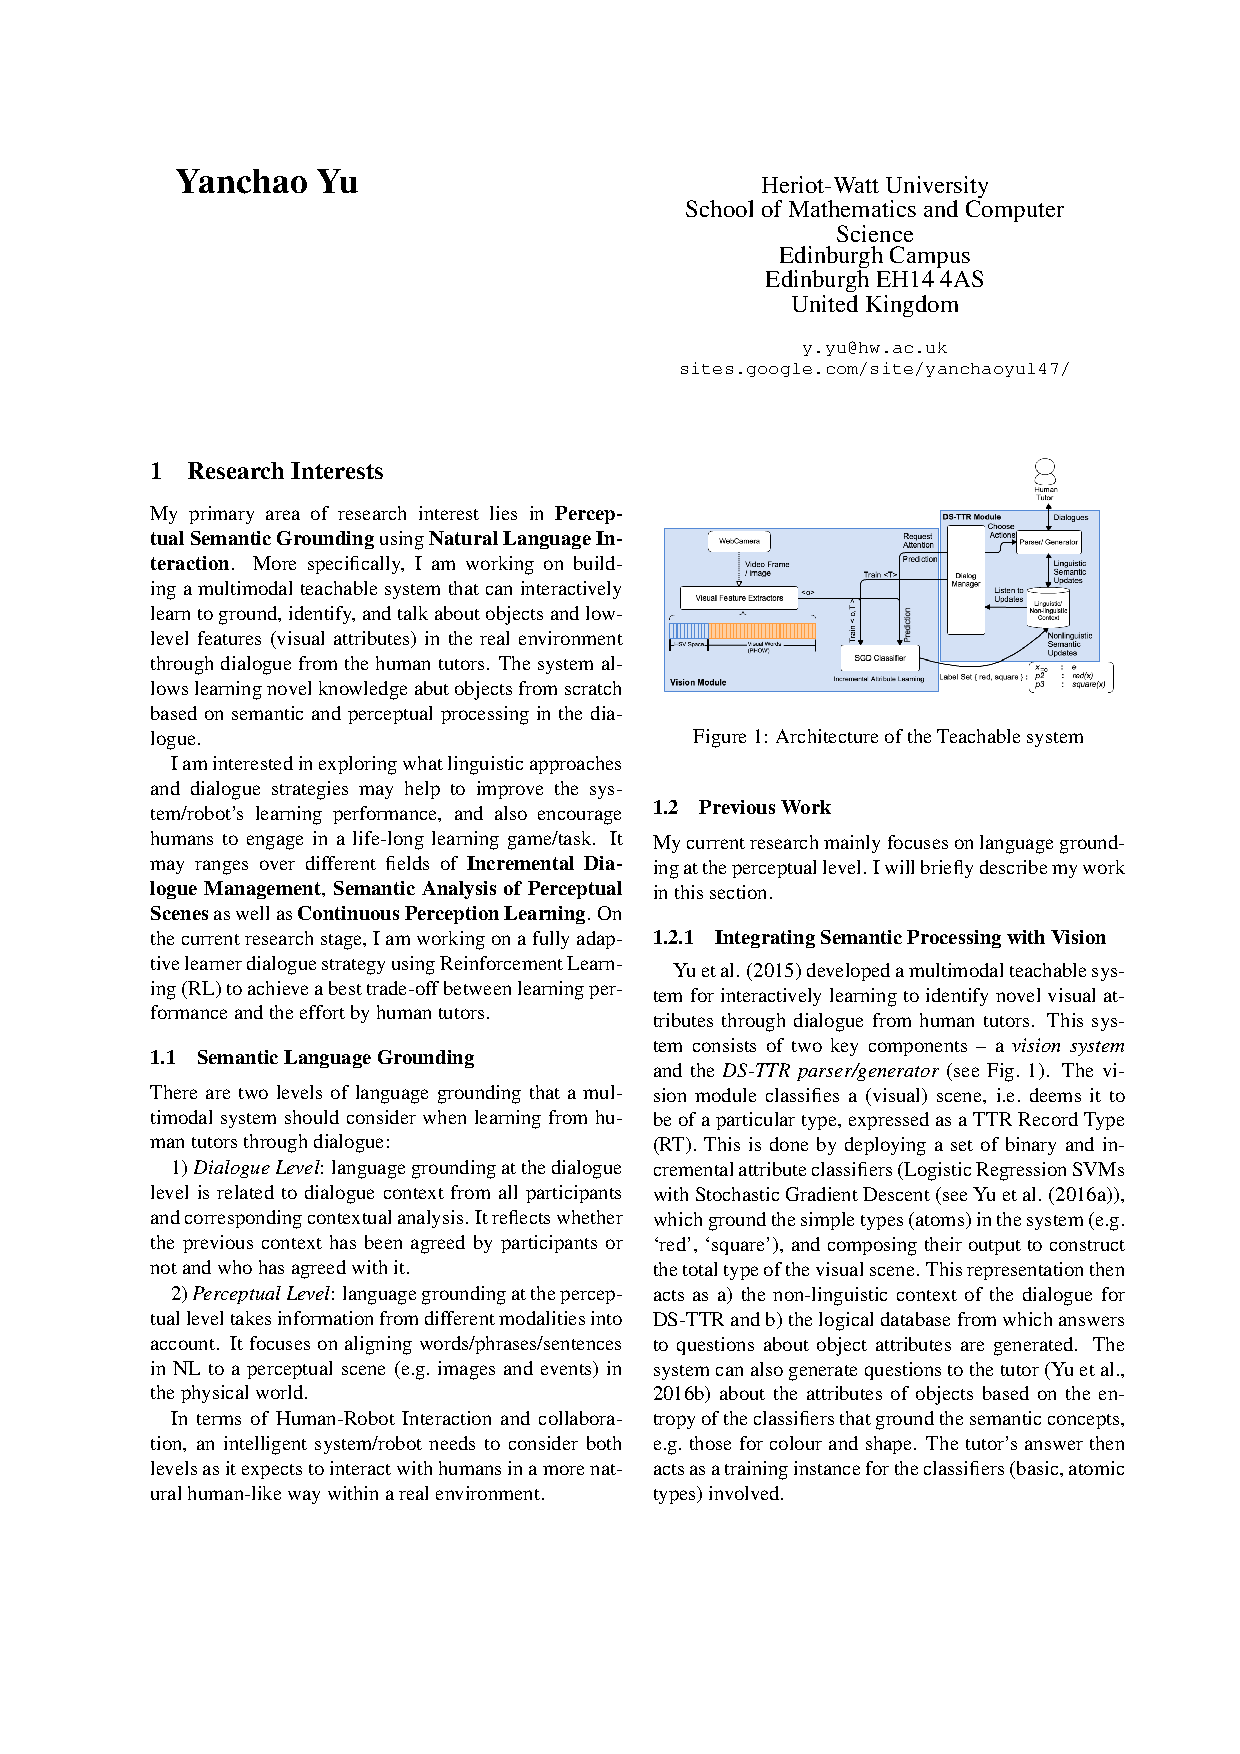
\includepdf[pages=-,pagecommand={},width=\textwidth]{YRRSDS_2016_paper_8_uanchao_yu.pdf}
% 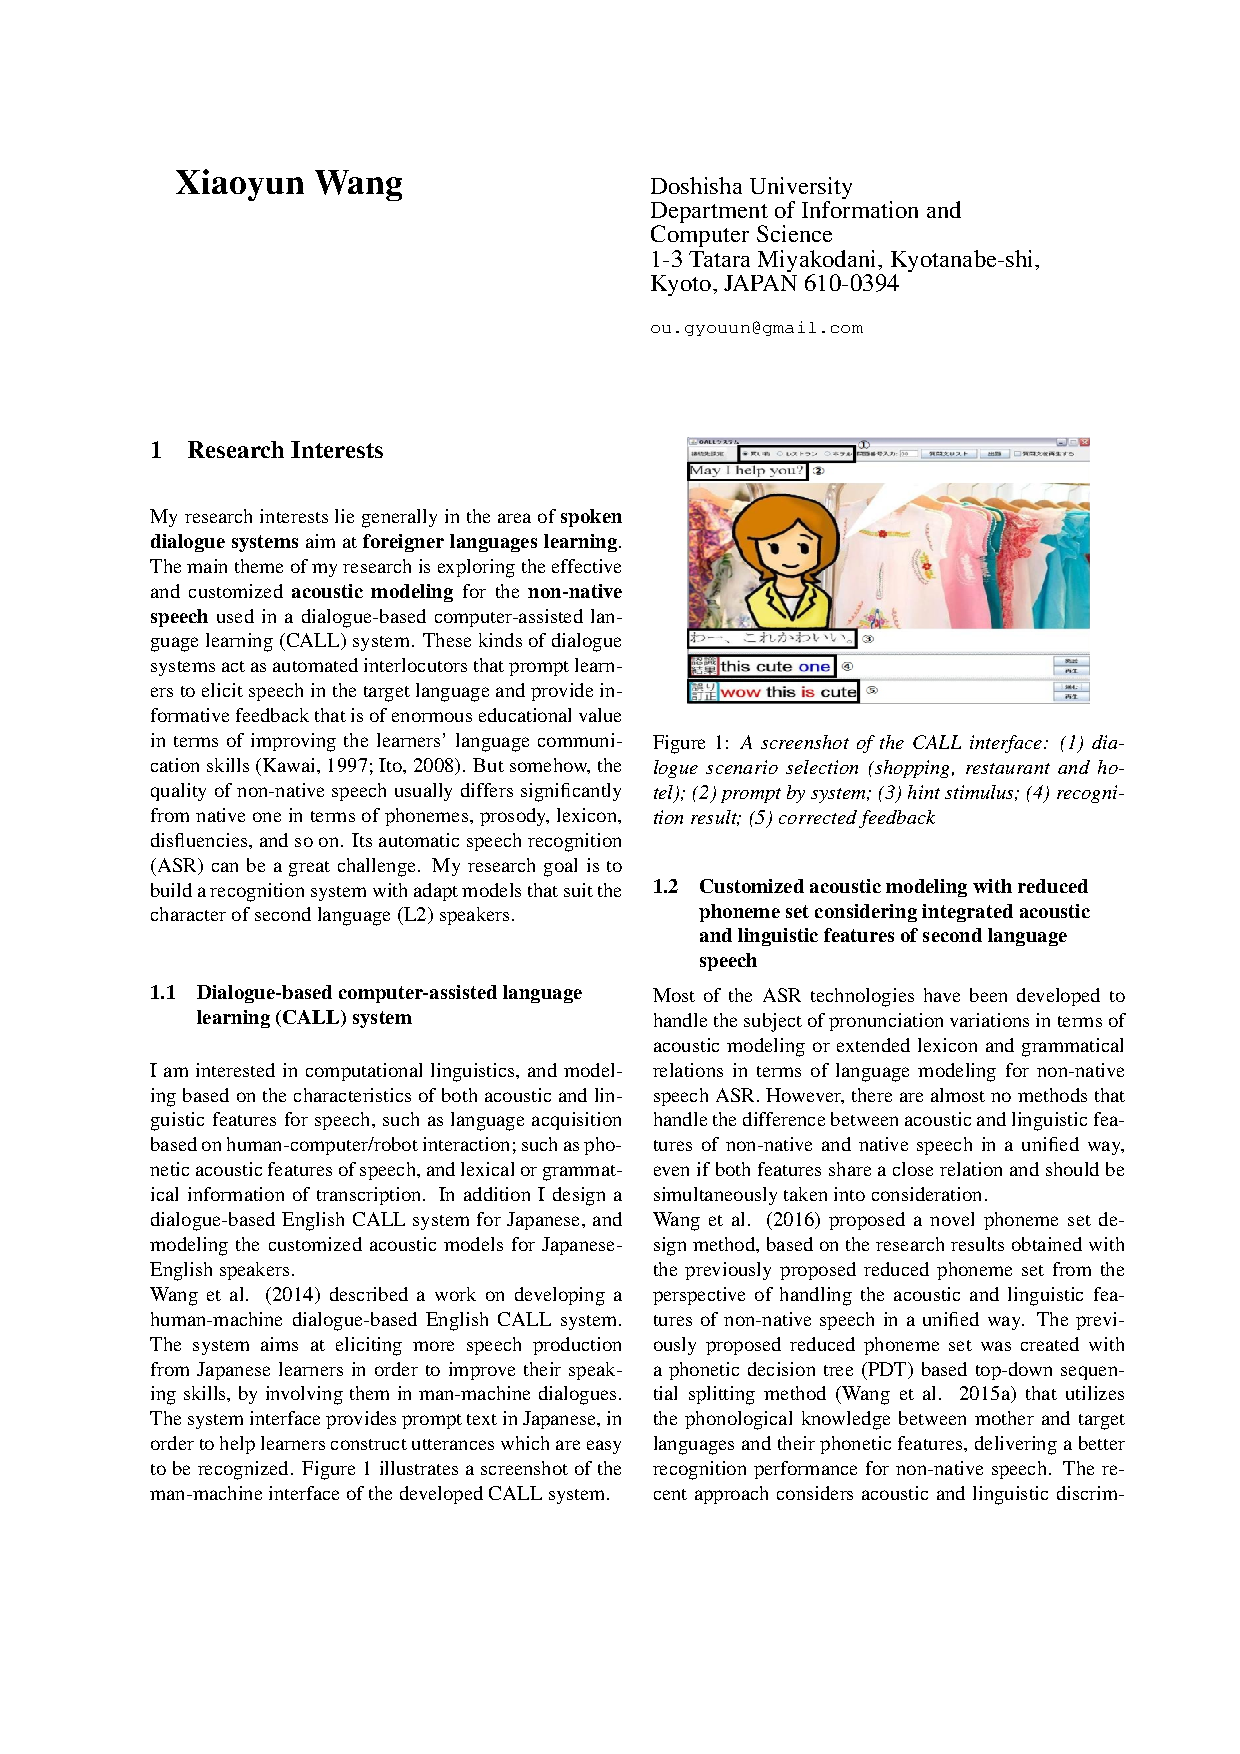
\includepdf[pages=-,pagecommand={},width=\textwidth]{YRRSDS_2016_paper_9_xiaoyun_wang.pdf}
% 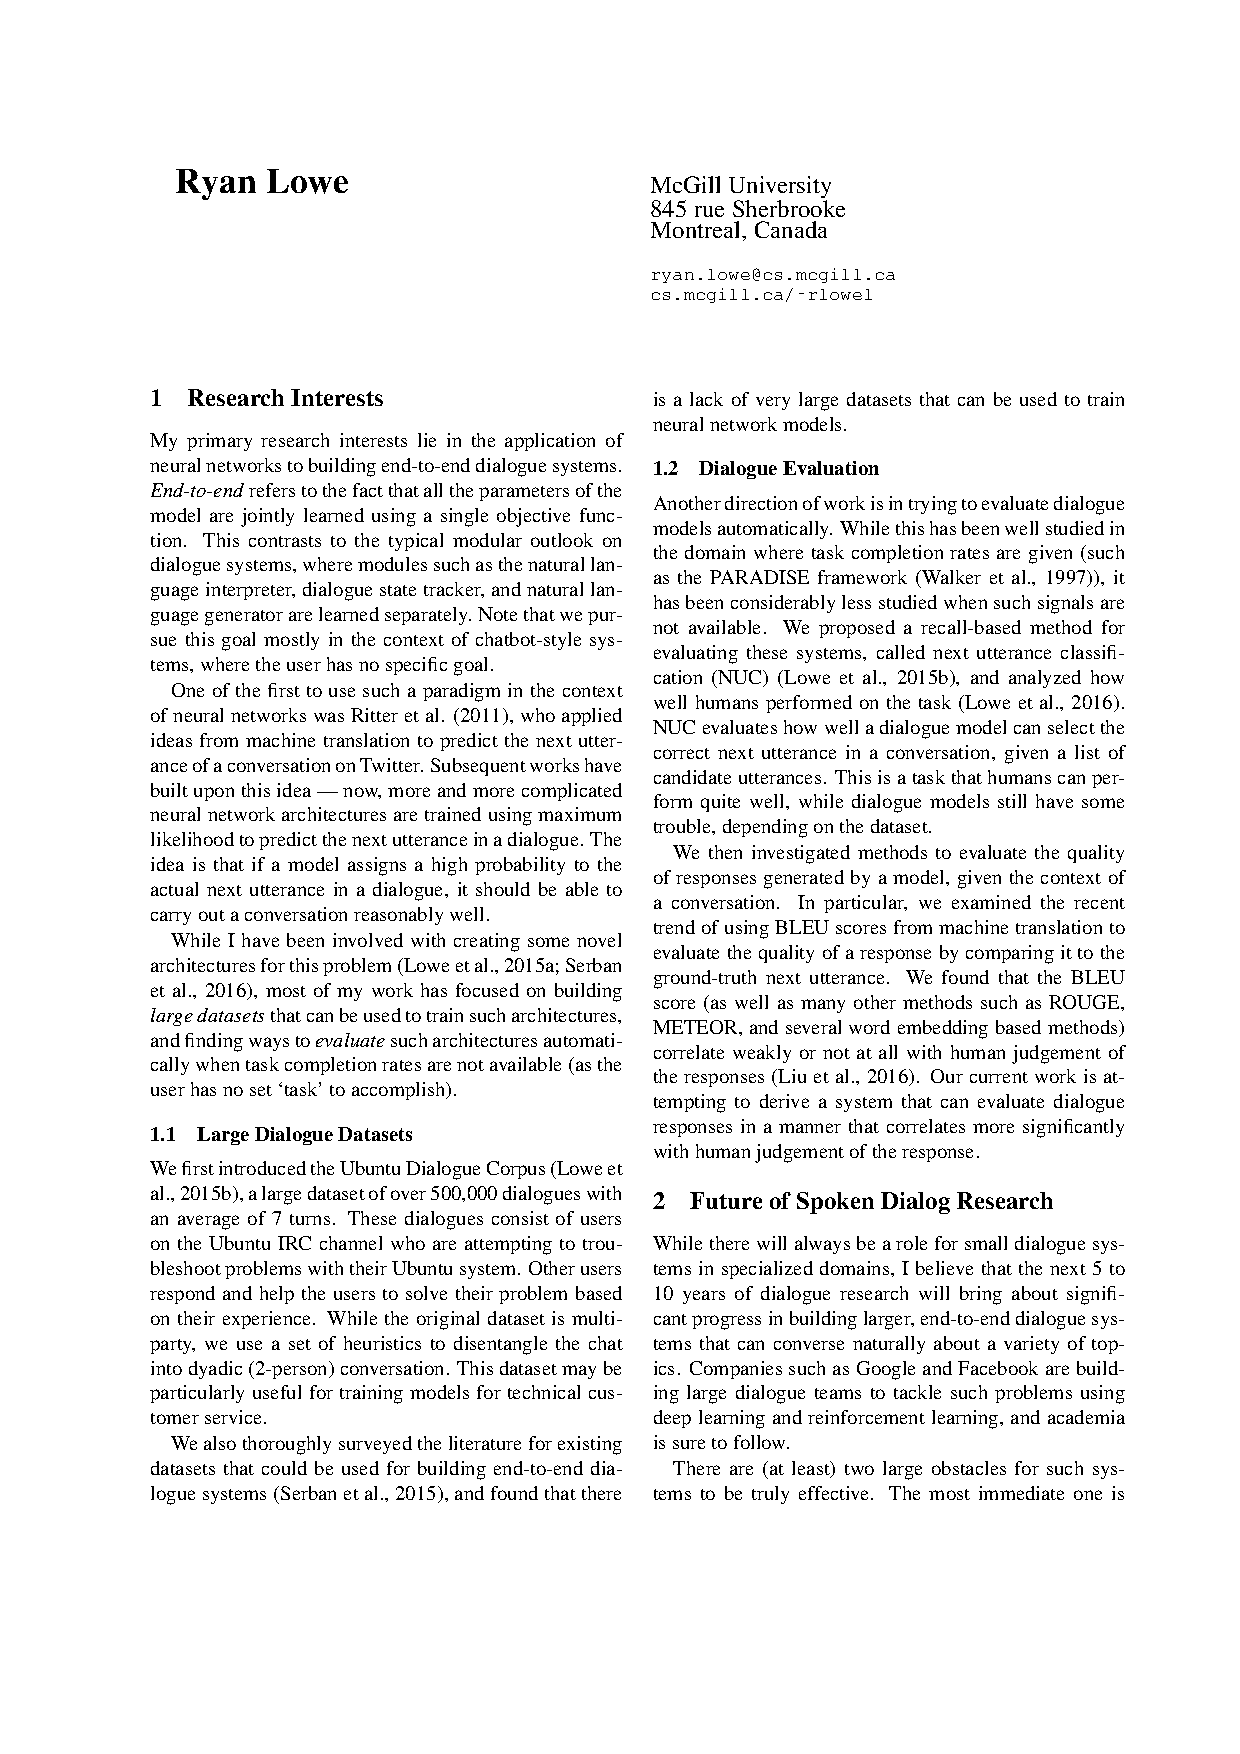
\includepdf[pages=-,pagecommand={},width=\textwidth]{YRRSDS_2016_paper_10_rayn_lowe.pdf}
% 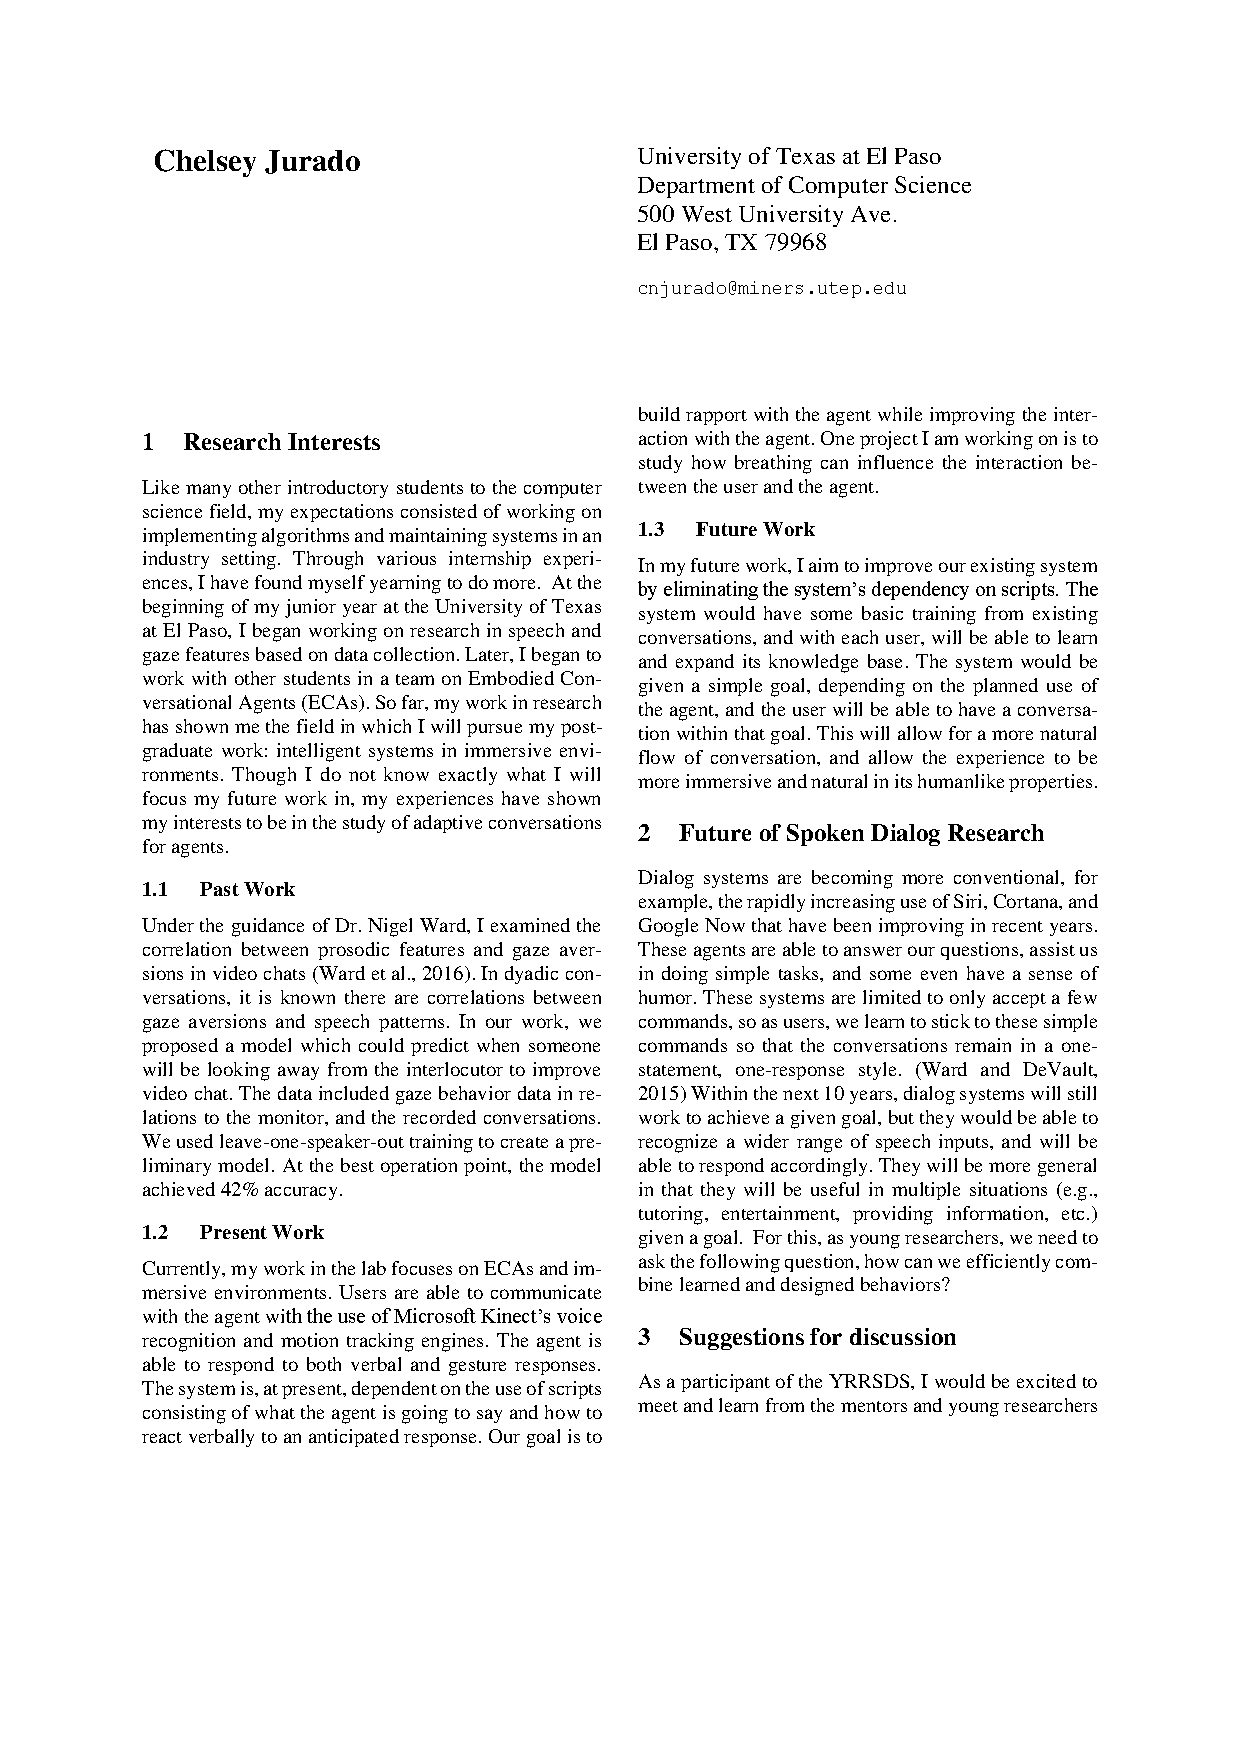
\includepdf[pages=-,pagecommand={},width=\textwidth]{YRRSDS_2016_paper_11_chelsey_jurado.pdf}
% 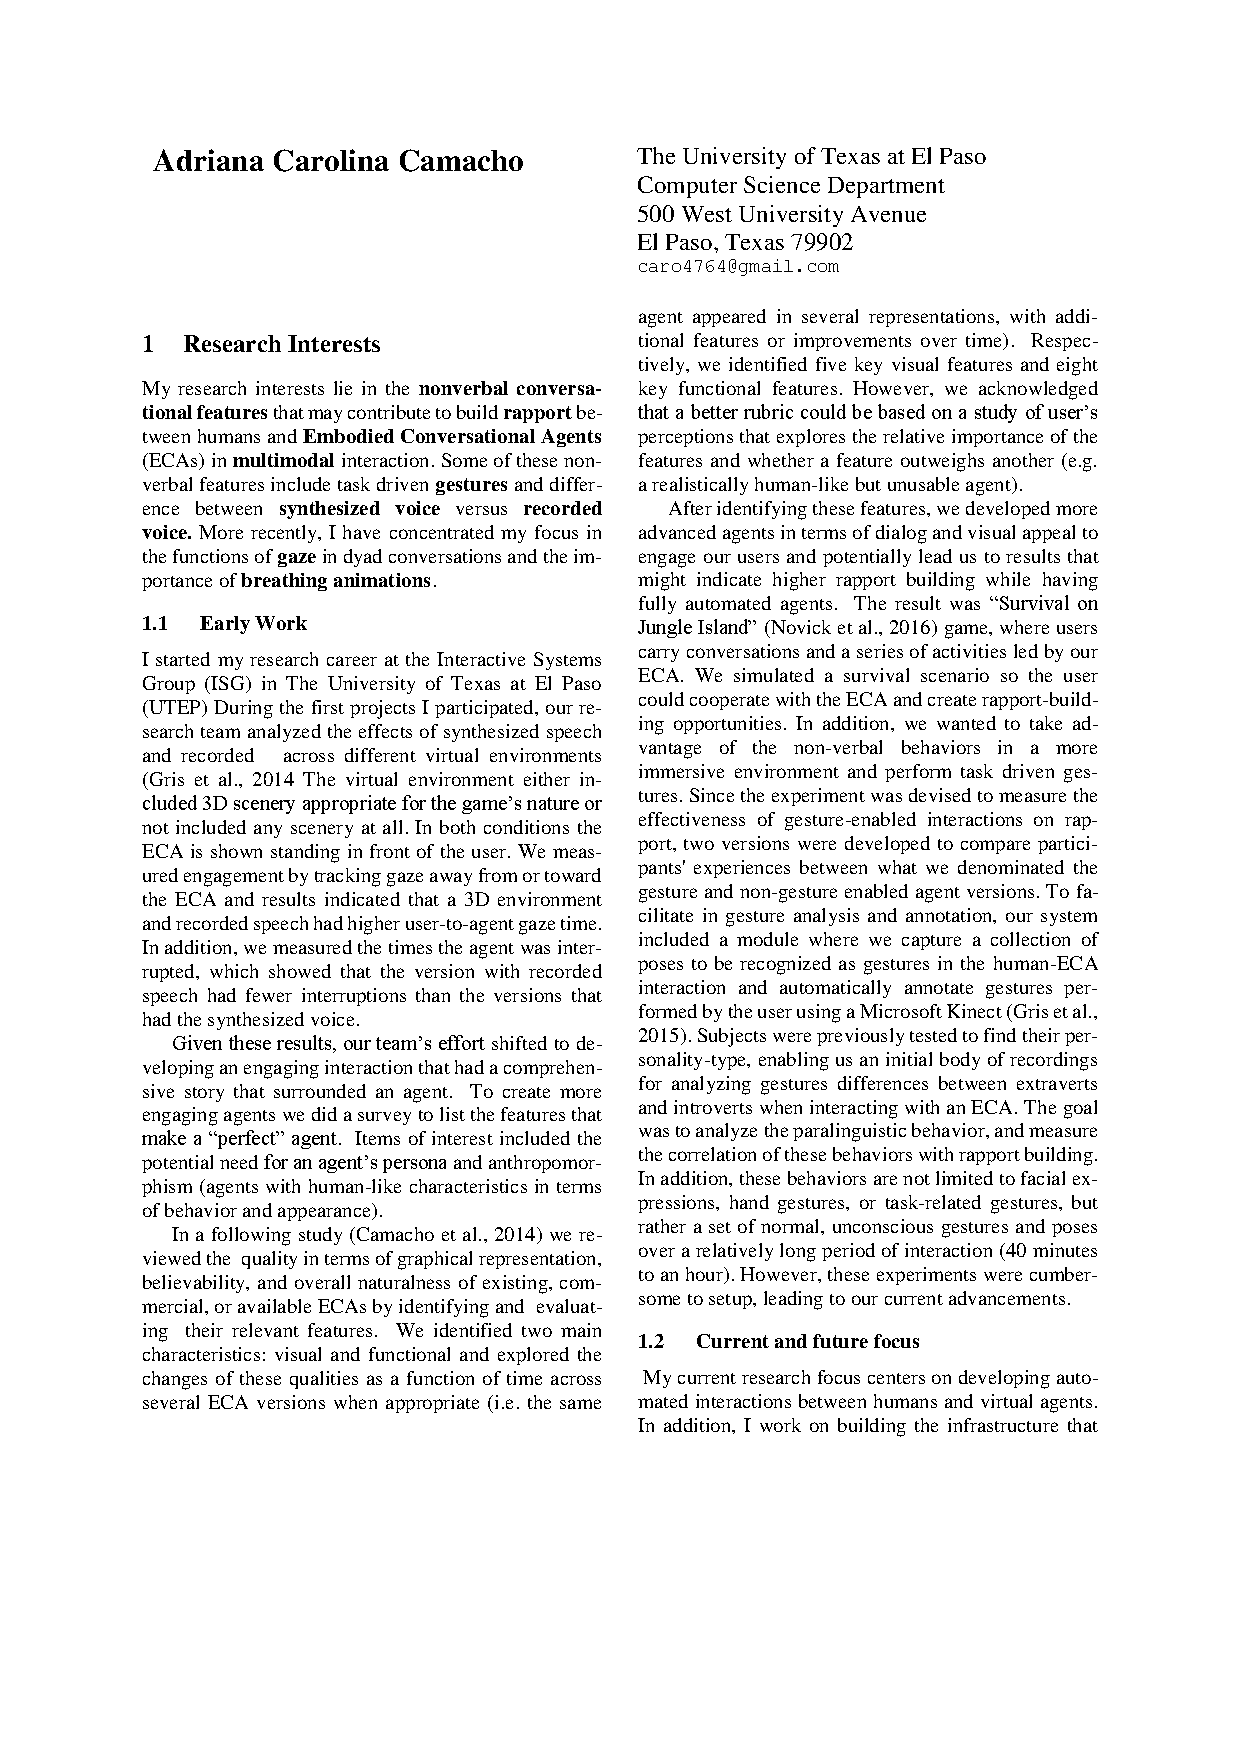
\includepdf[pages=-,pagecommand={},width=\textwidth]{YRRSDS_2016_paper_12_adriana_camacho.pdf}
% 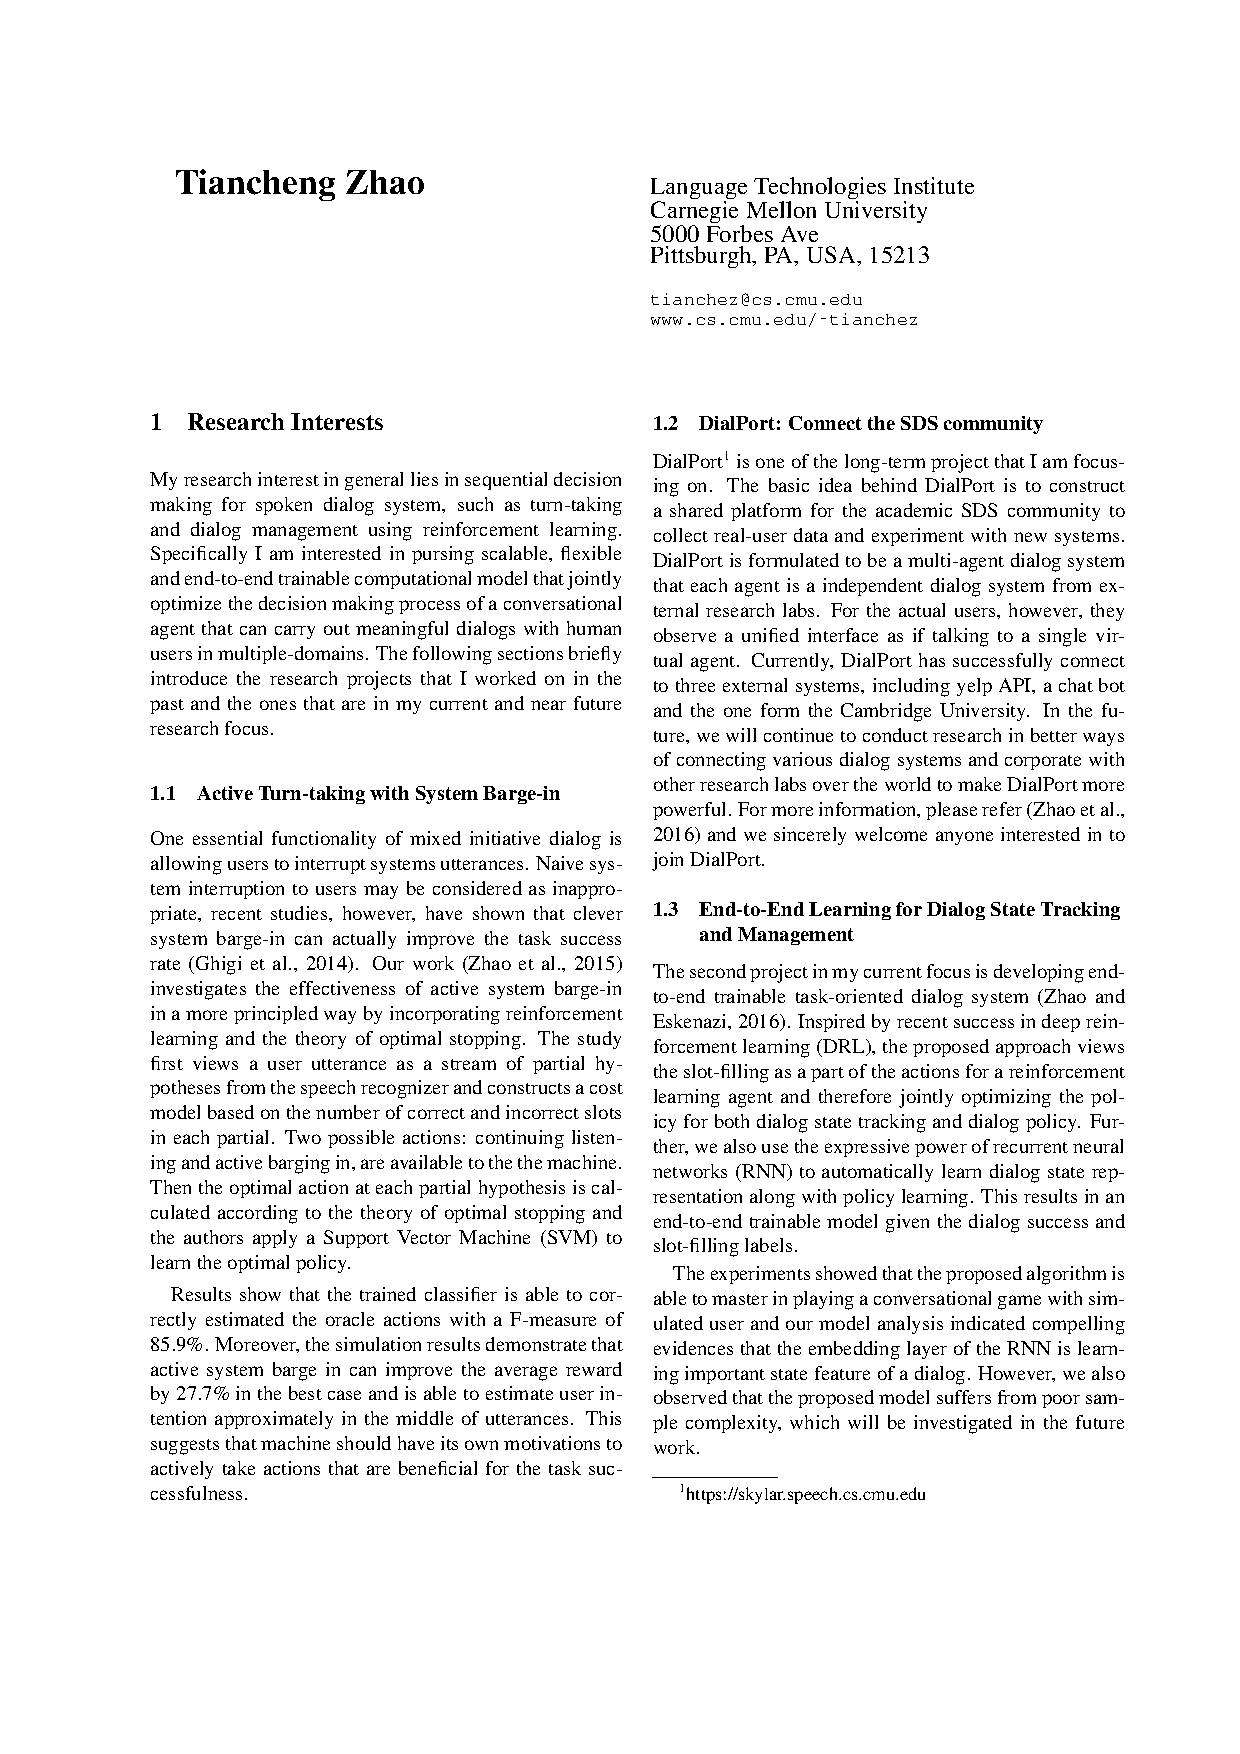
\includepdf[pages=-,pagecommand={},width=\textwidth]{YRRSDS_2016_paper_14_tiancheng_zhao.pdf}
% 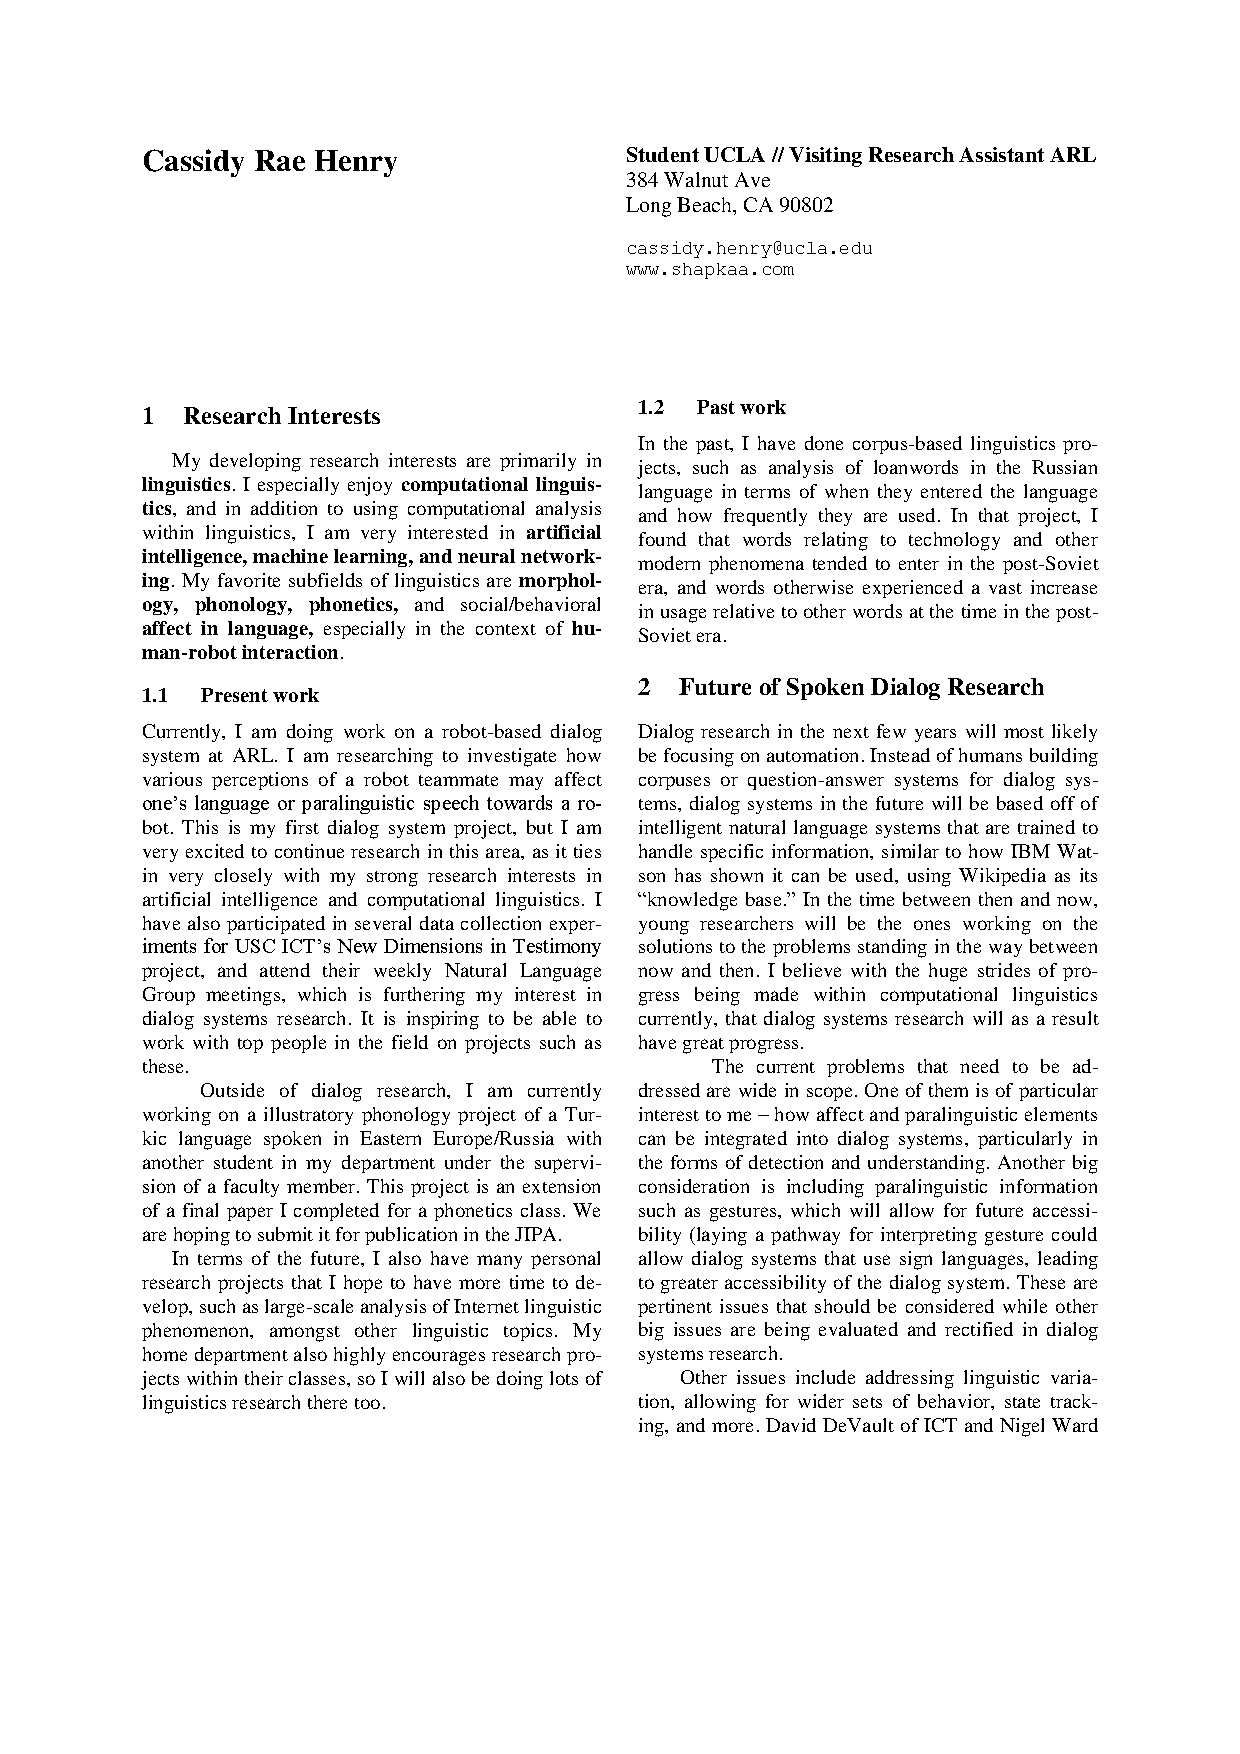
\includepdf[pages=-,pagecommand={},width=\textwidth]{YRRSDS_2016_paper_15_cassidy_henry.pdf}
% 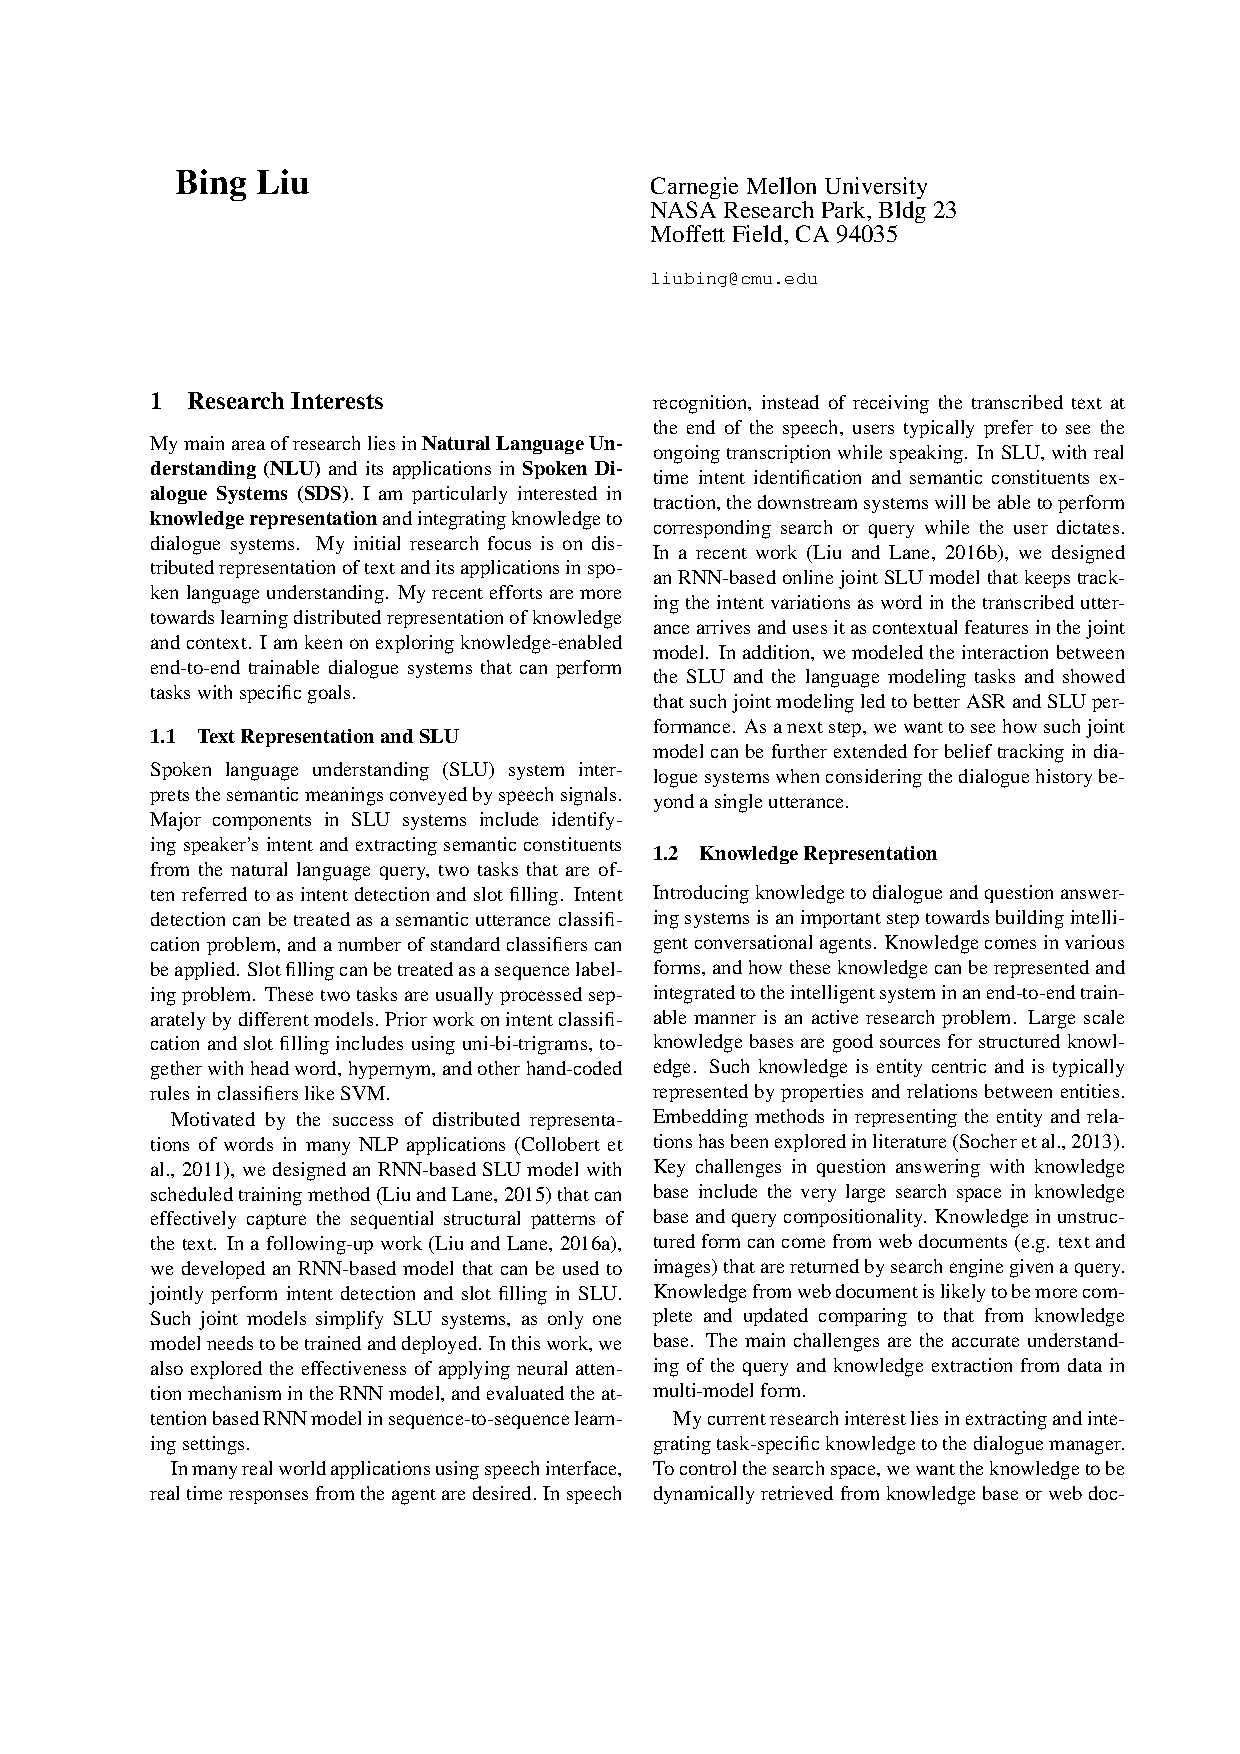
\includepdf[pages=-,pagecommand={},width=\textwidth]{YRRSDS_2016_paper_16_bing_liu.pdf}
% 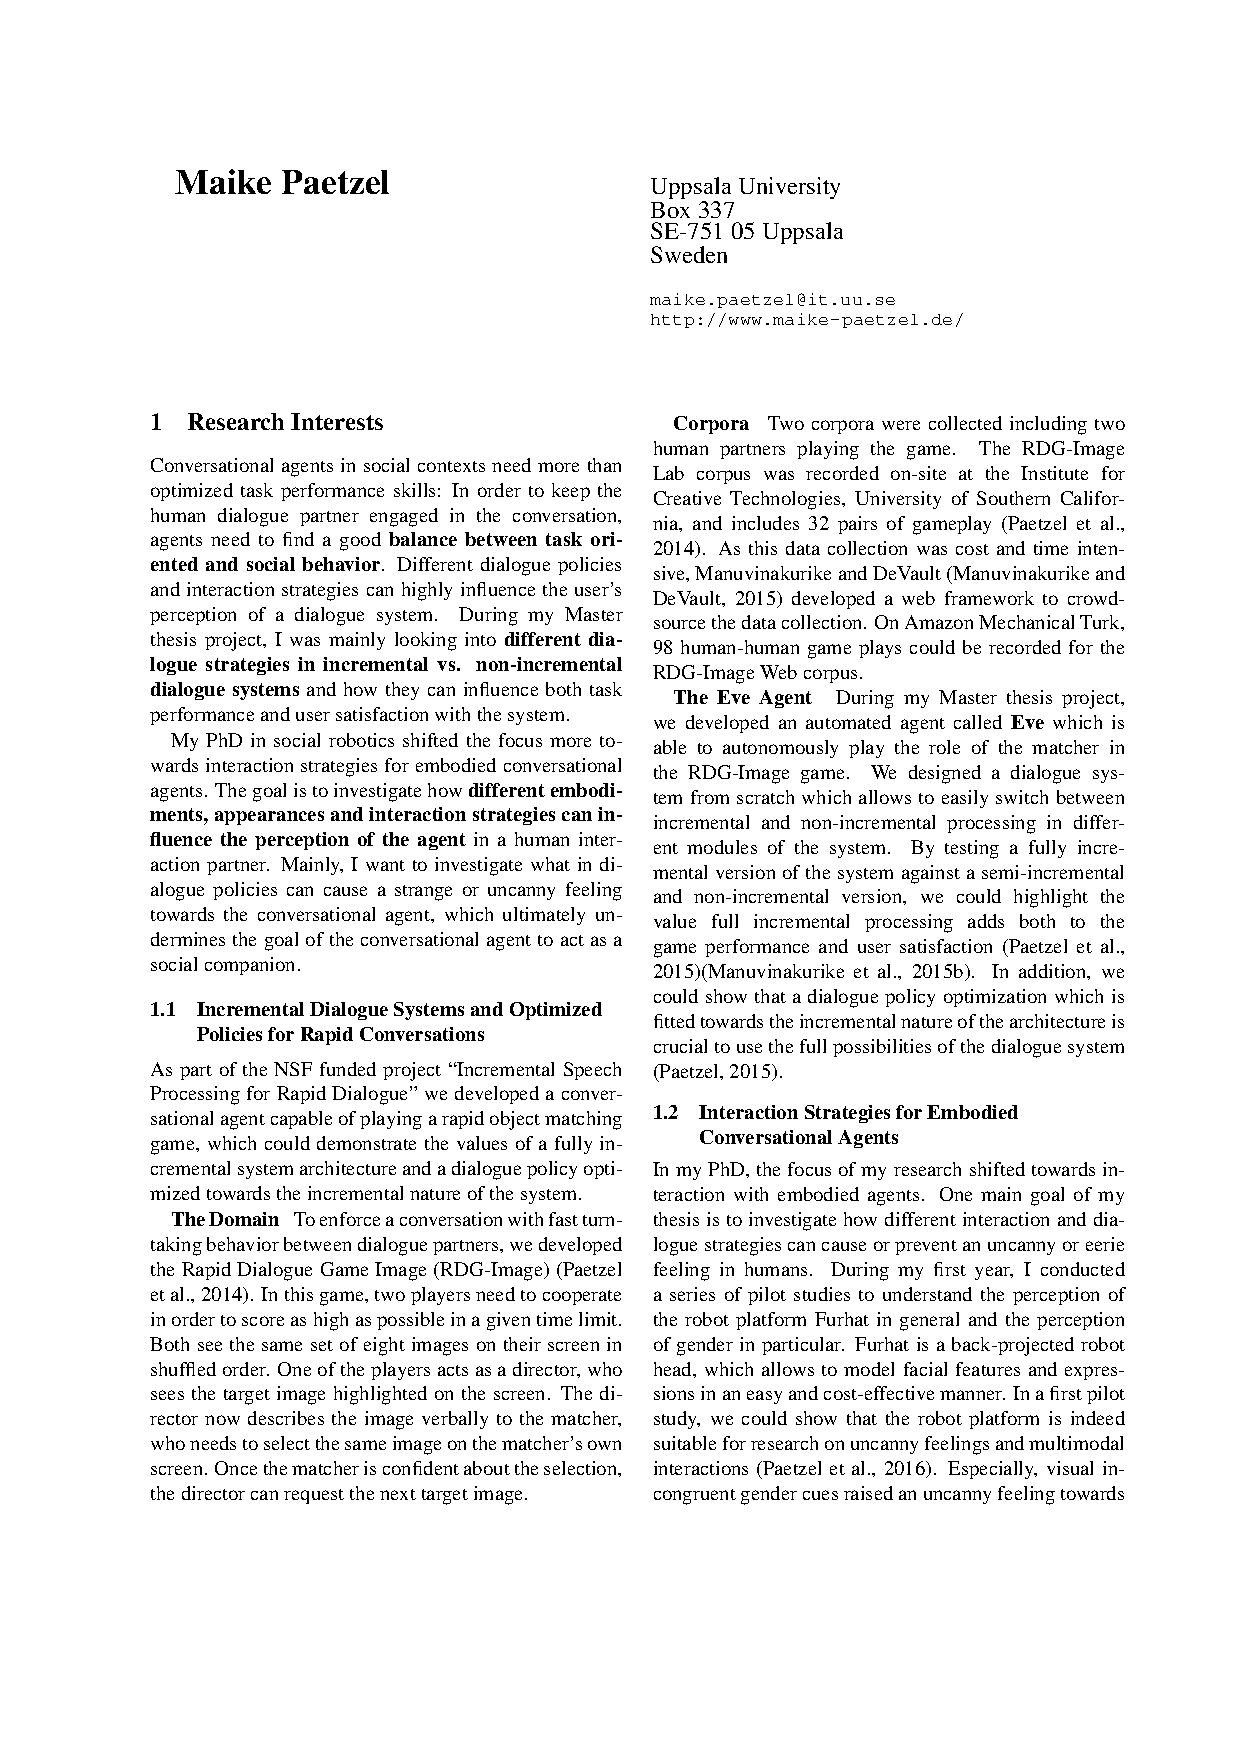
\includepdf[pages=-,pagecommand={},width=\textwidth]{YRRSDS_2016_paper_17_maike_paetzel.pdf}
% 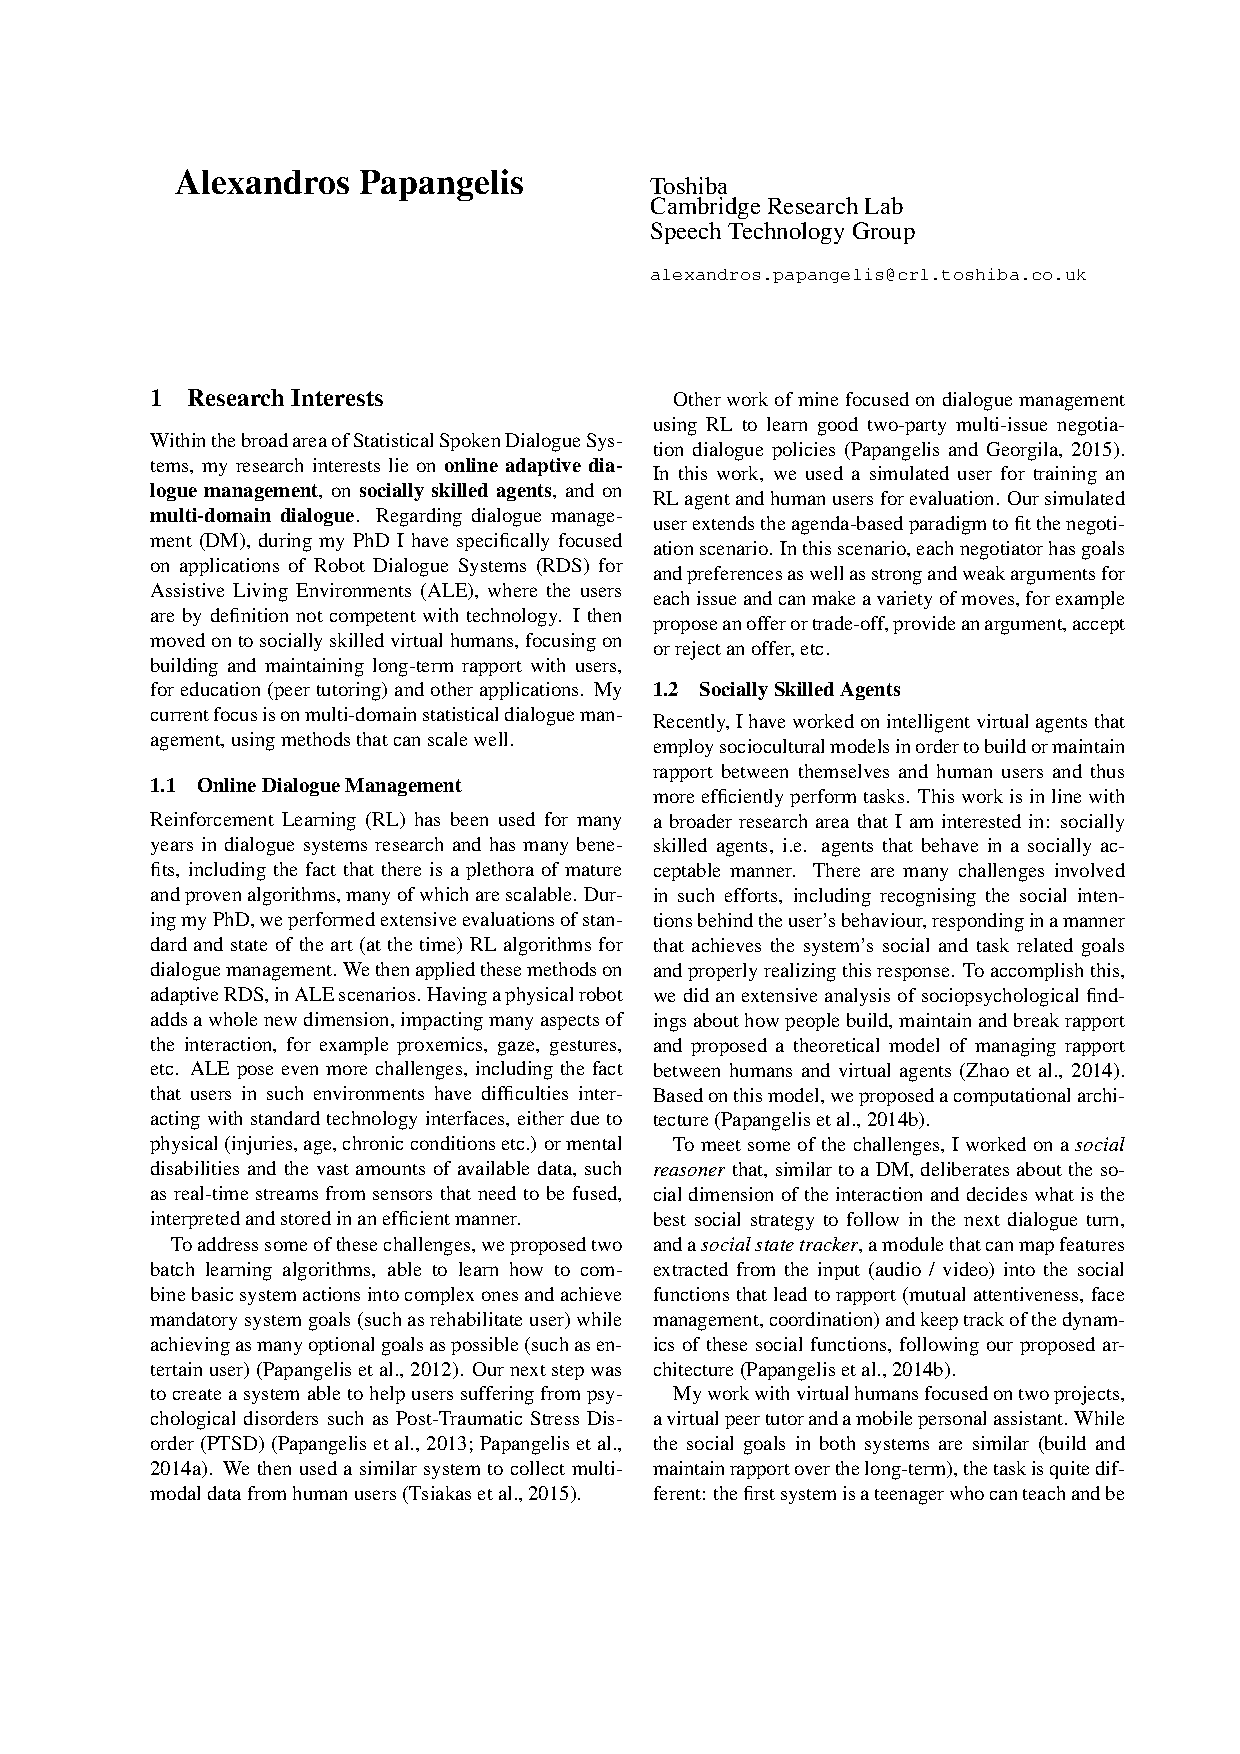
\includepdf[pages=-,pagecommand={},width=\textwidth]{YRRSDS_2016_paper_18_alexandros_papangelis.pdf}
% 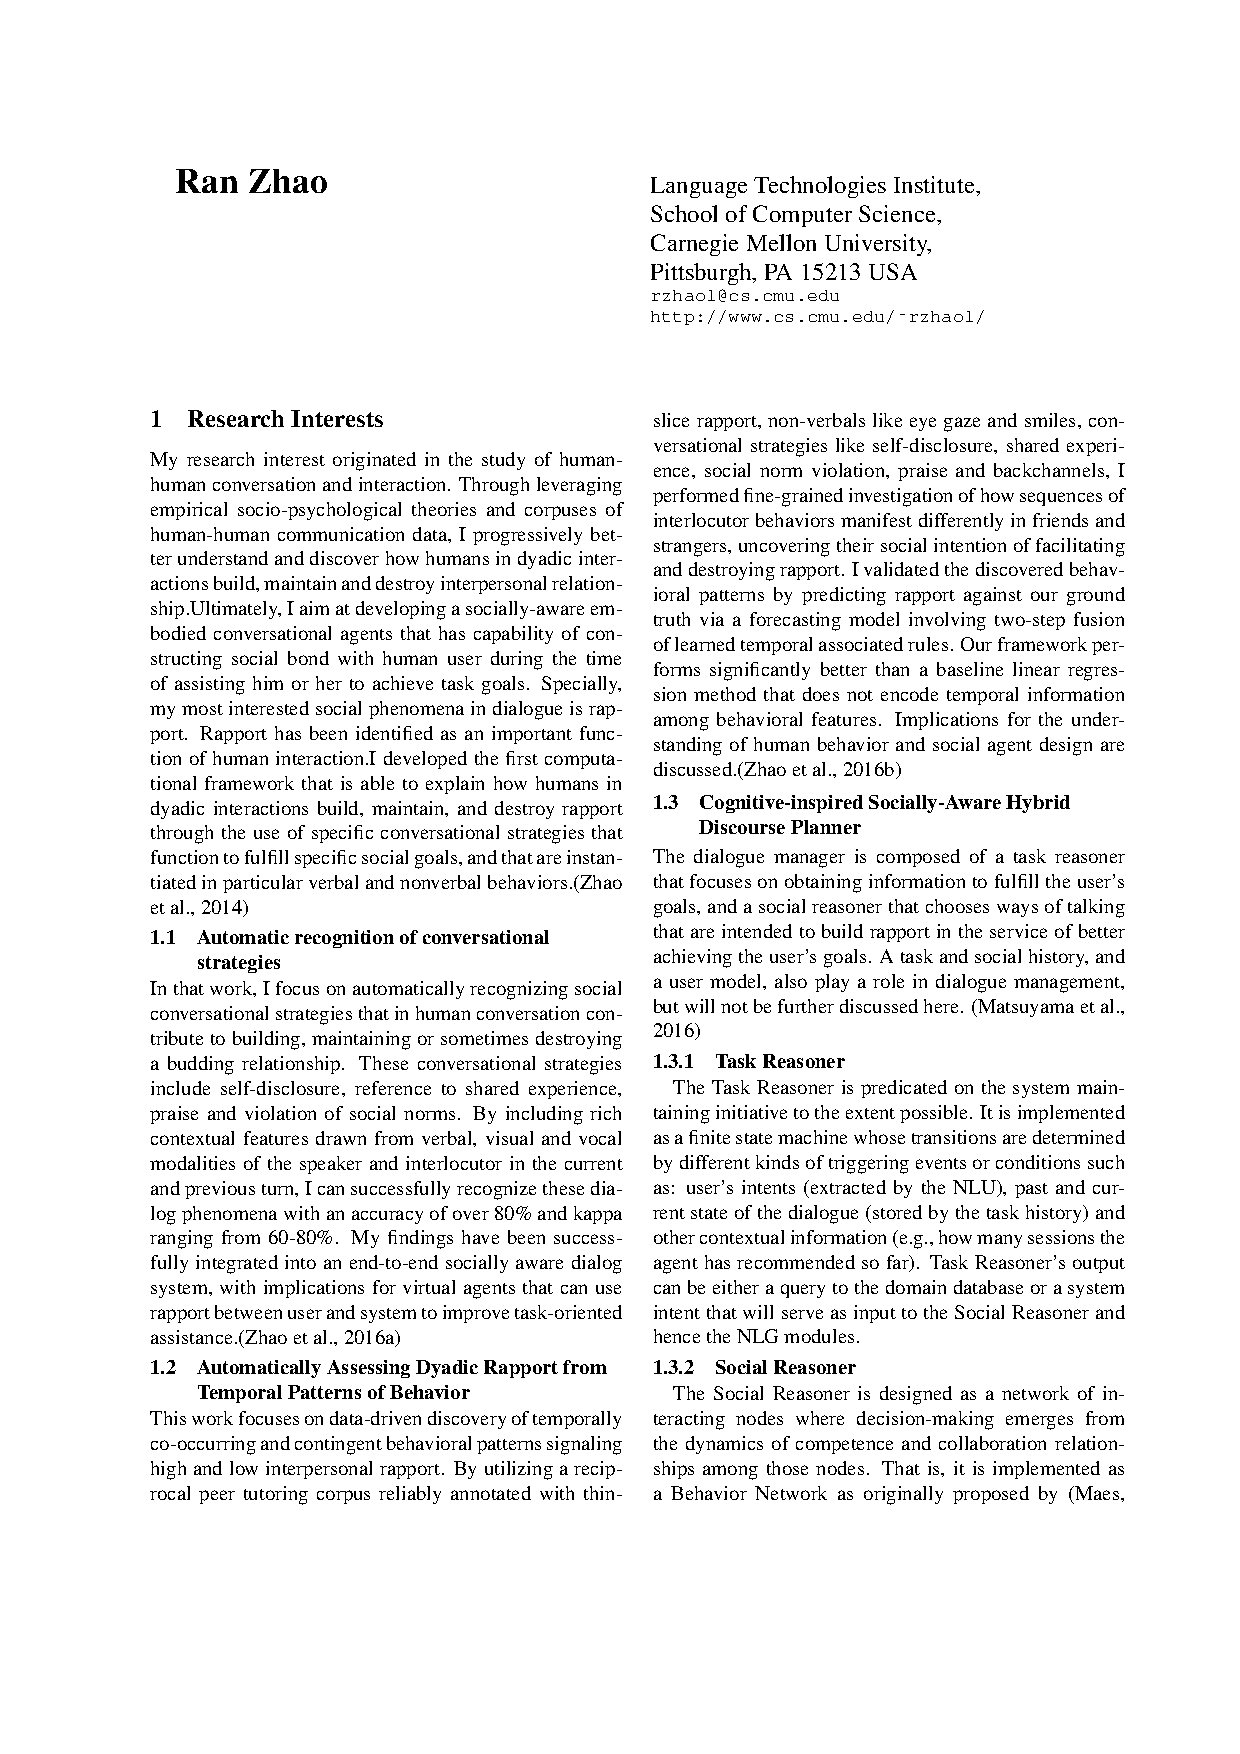
\includepdf[pages=-,pagecommand={},width=\textwidth]{YRRSDS_2016_paper_19_ran_zhao.pdf}
% 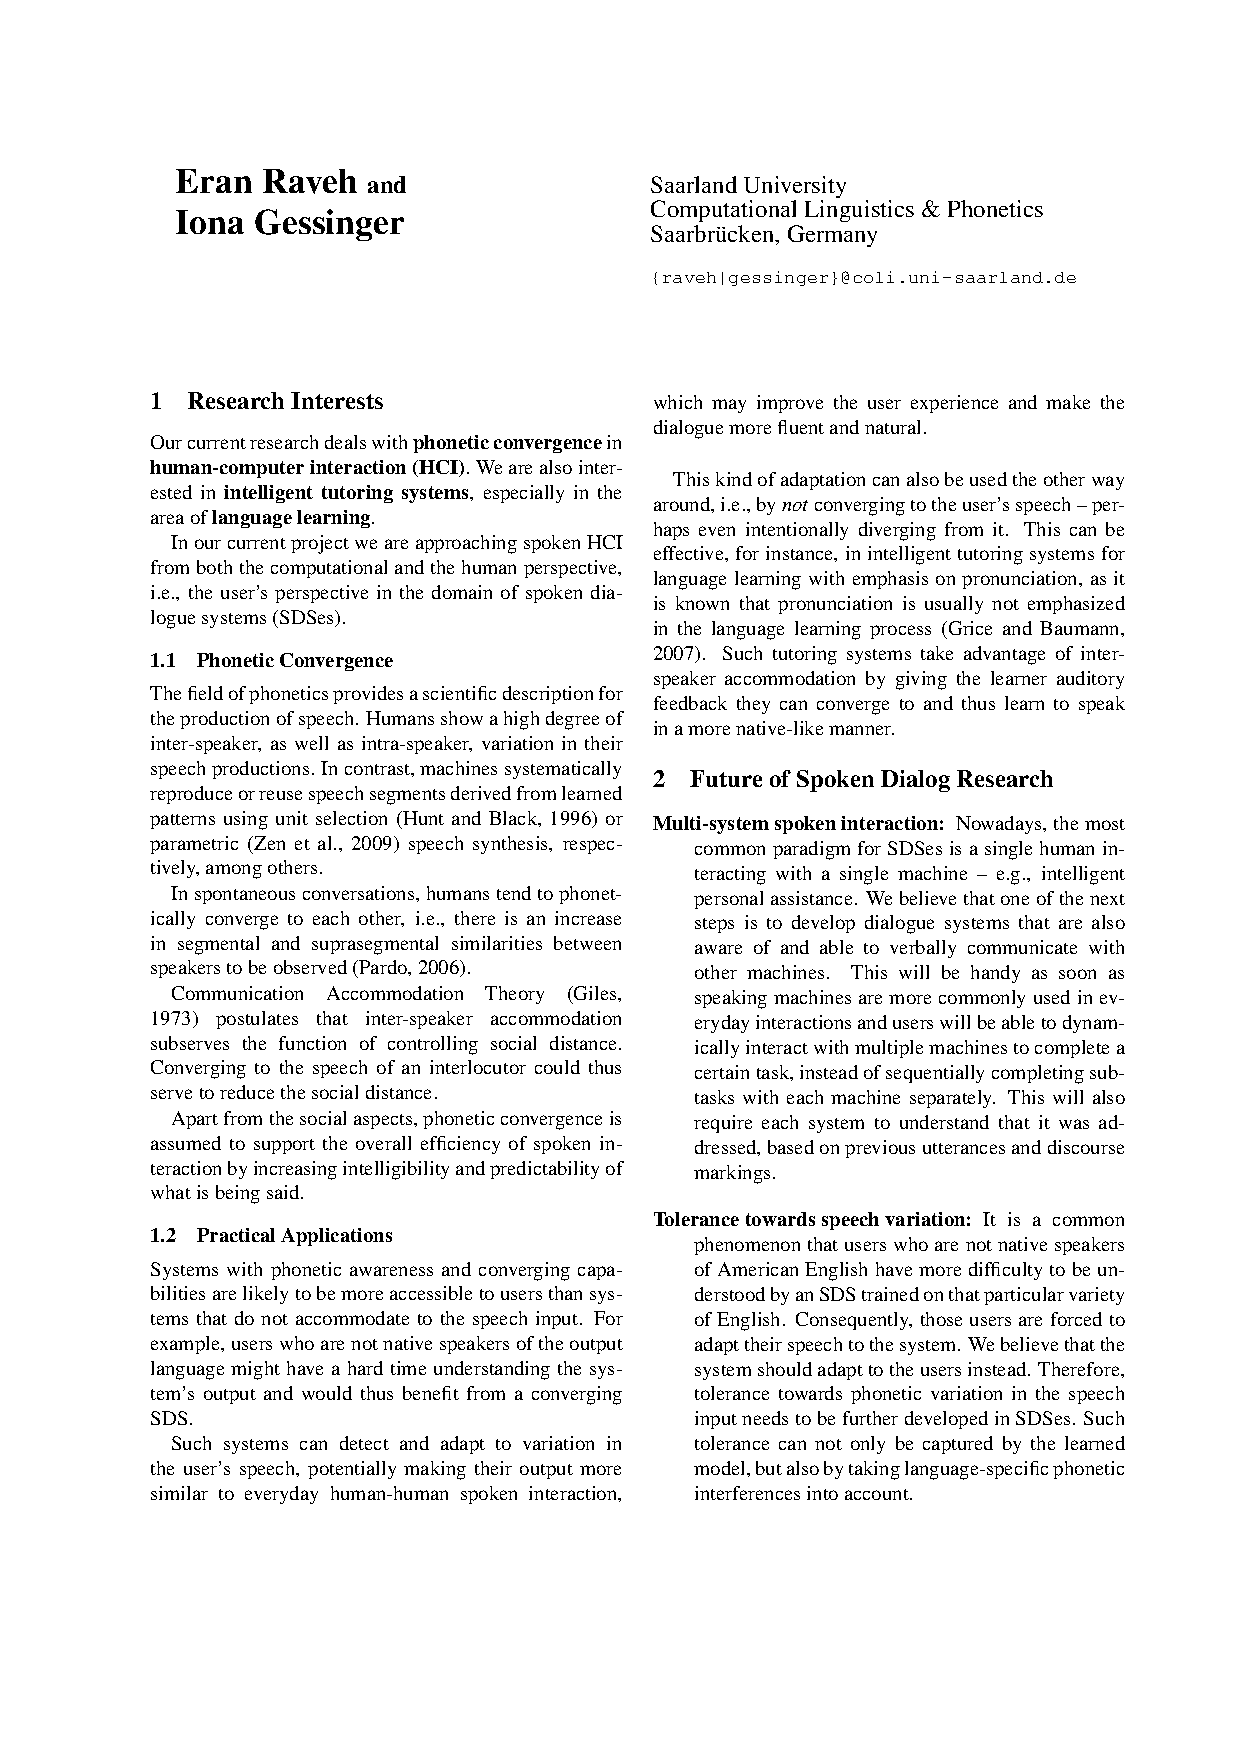
\includepdf[pages=-,pagecommand={},width=\textwidth]{YRRSDS_2016_paper_20_eran_raveh_iona_gessinger.pdf}
% 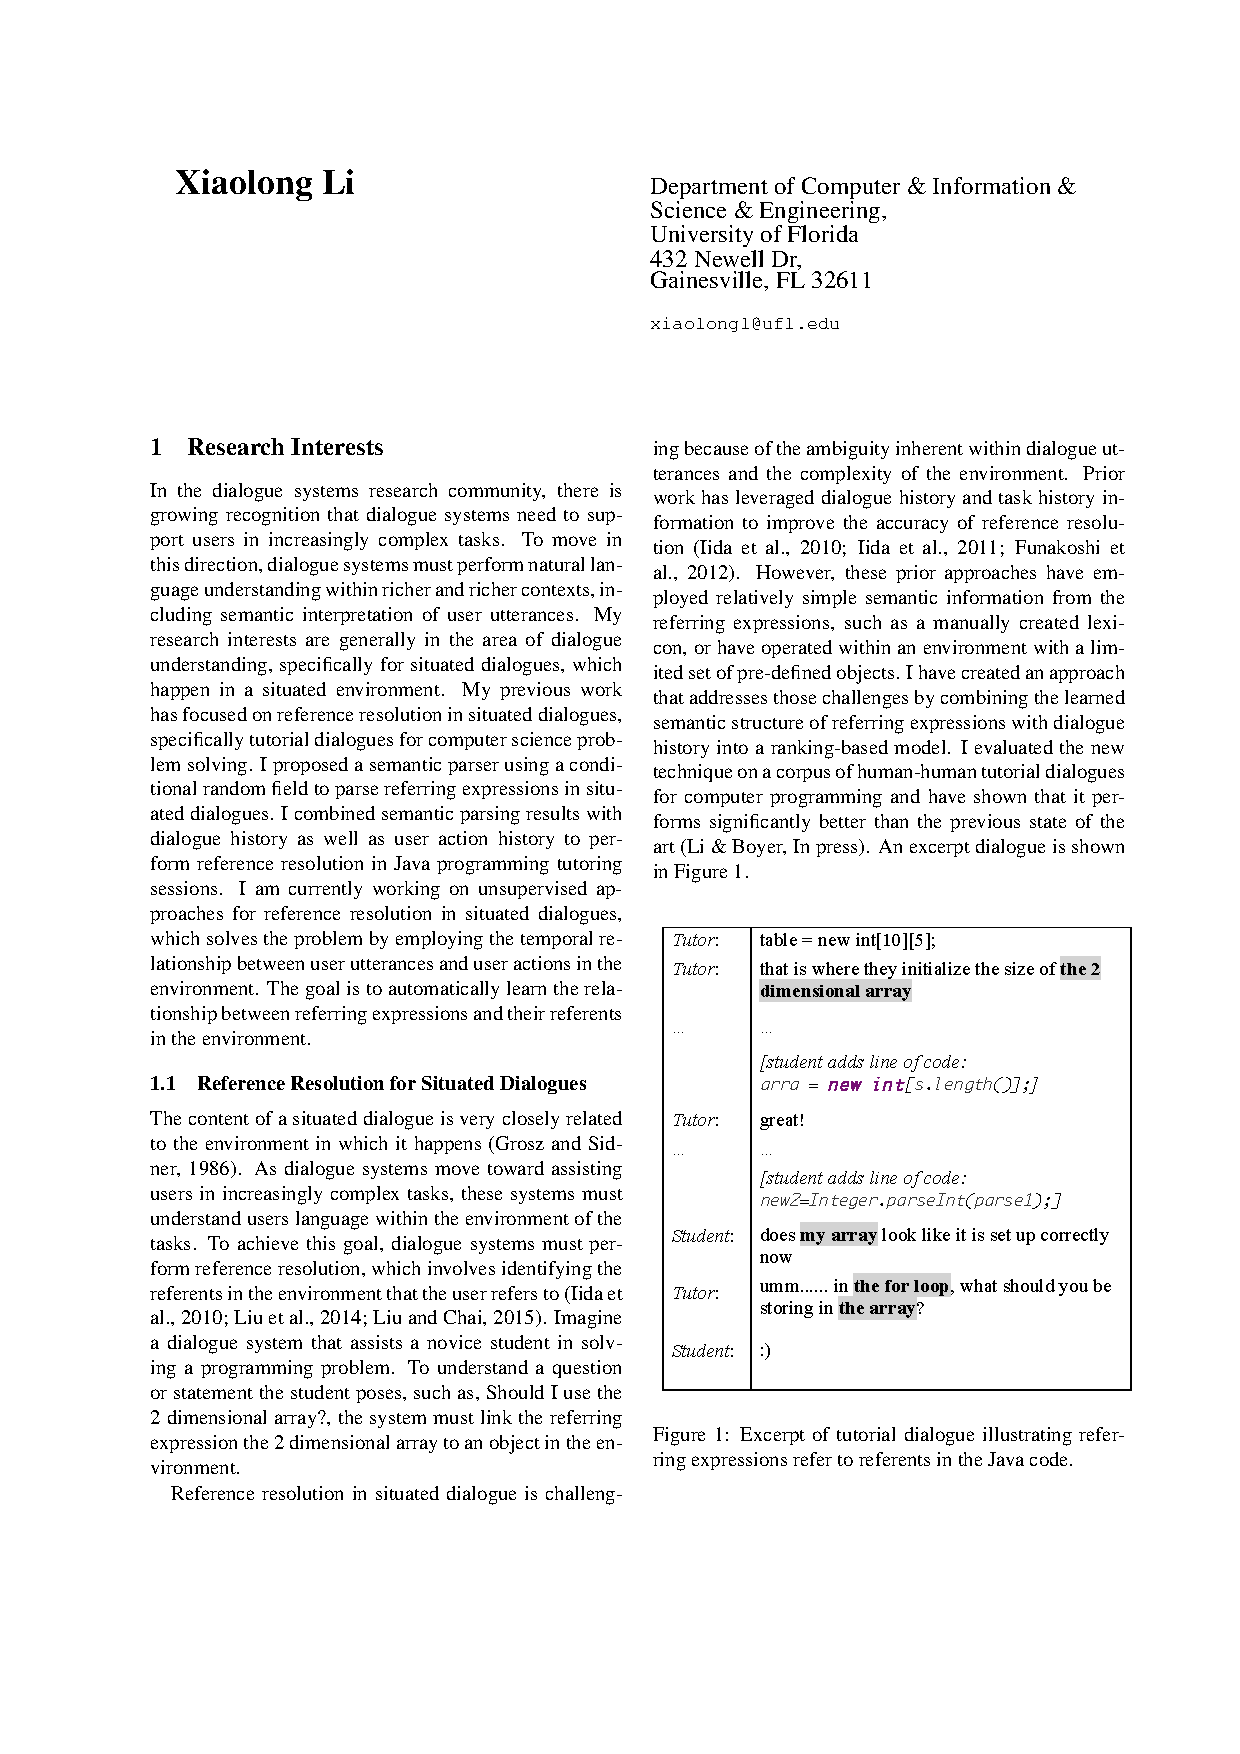
\includepdf[pages=-,pagecommand={},width=\textwidth]{YRRSDS_2016_paper_21_xialolong_li.pdf}
% 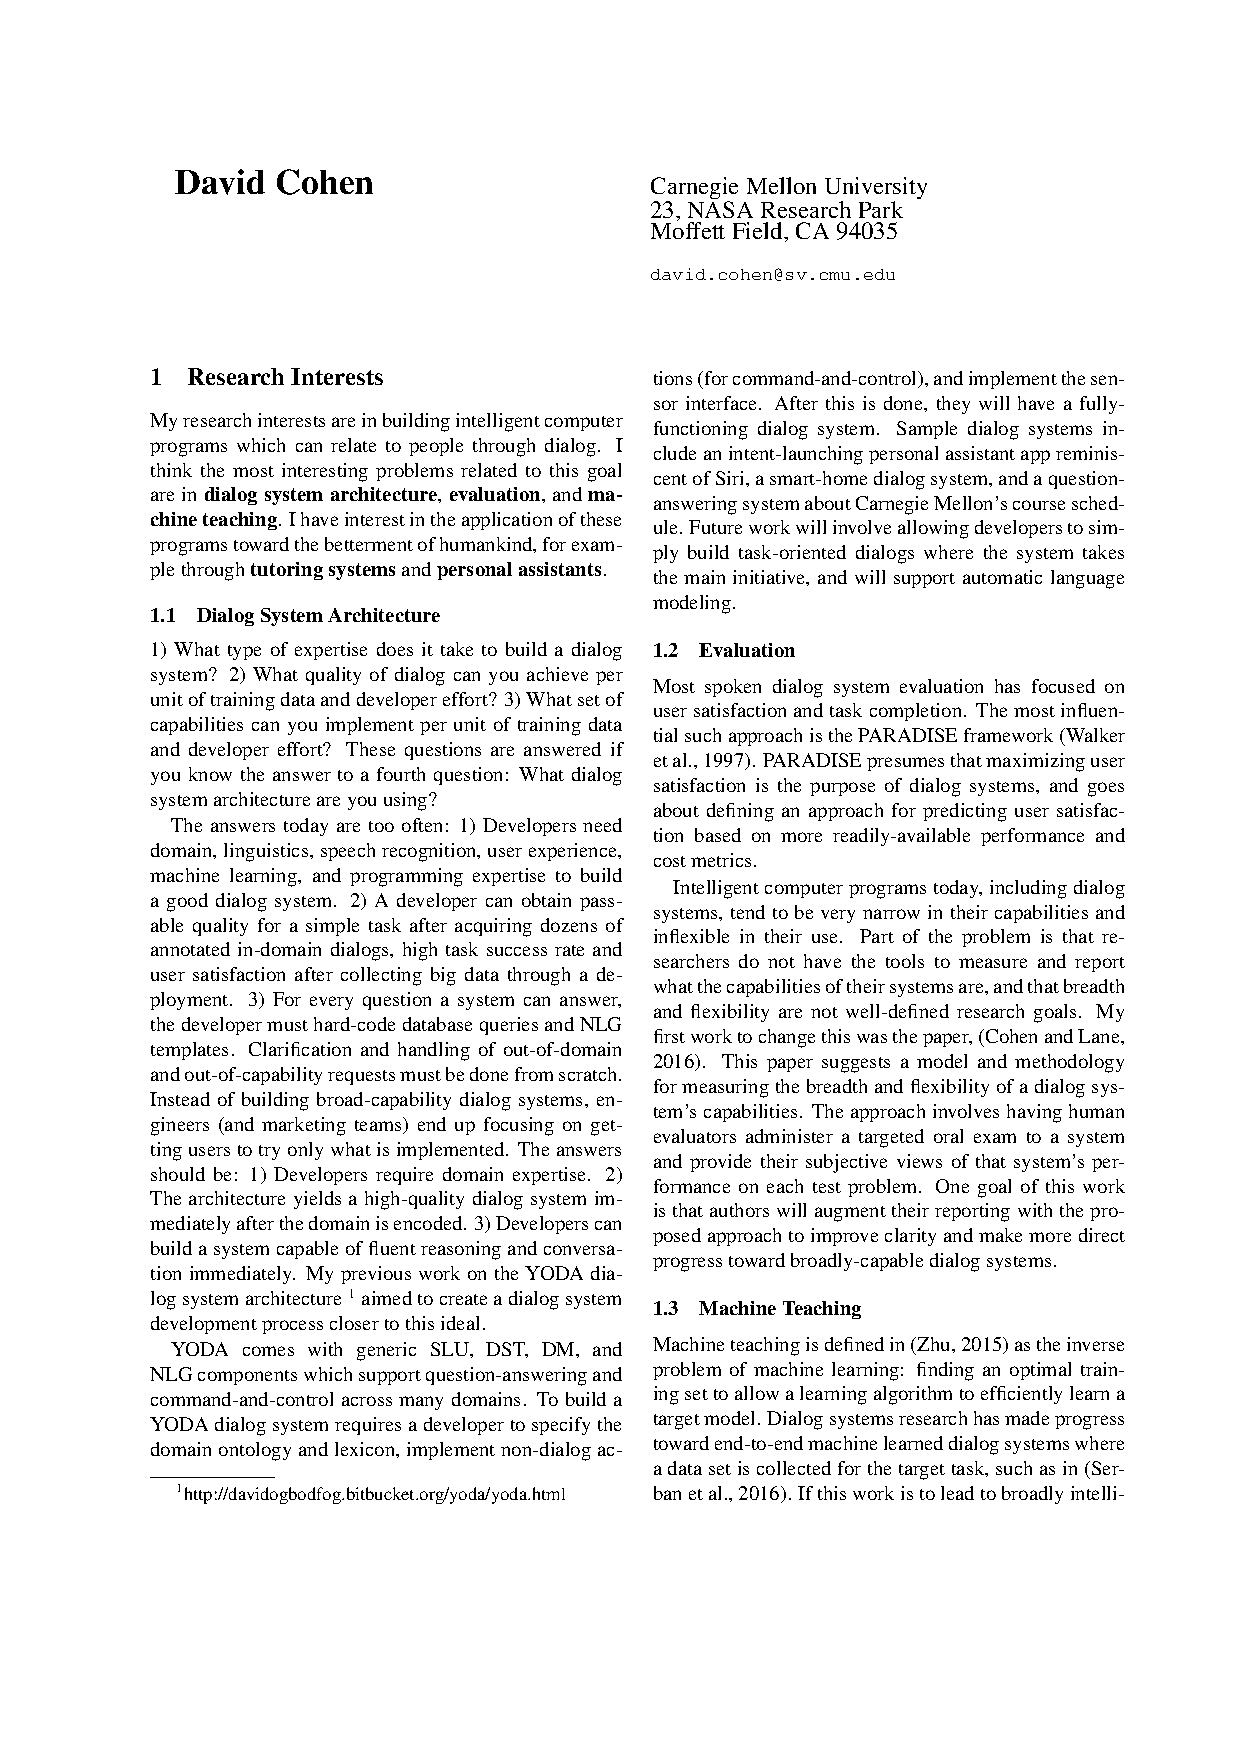
\includepdf[pages=-,pagecommand={},width=\textwidth]{YRRSDS_2016_paper_22_david_cohen.pdf}
% 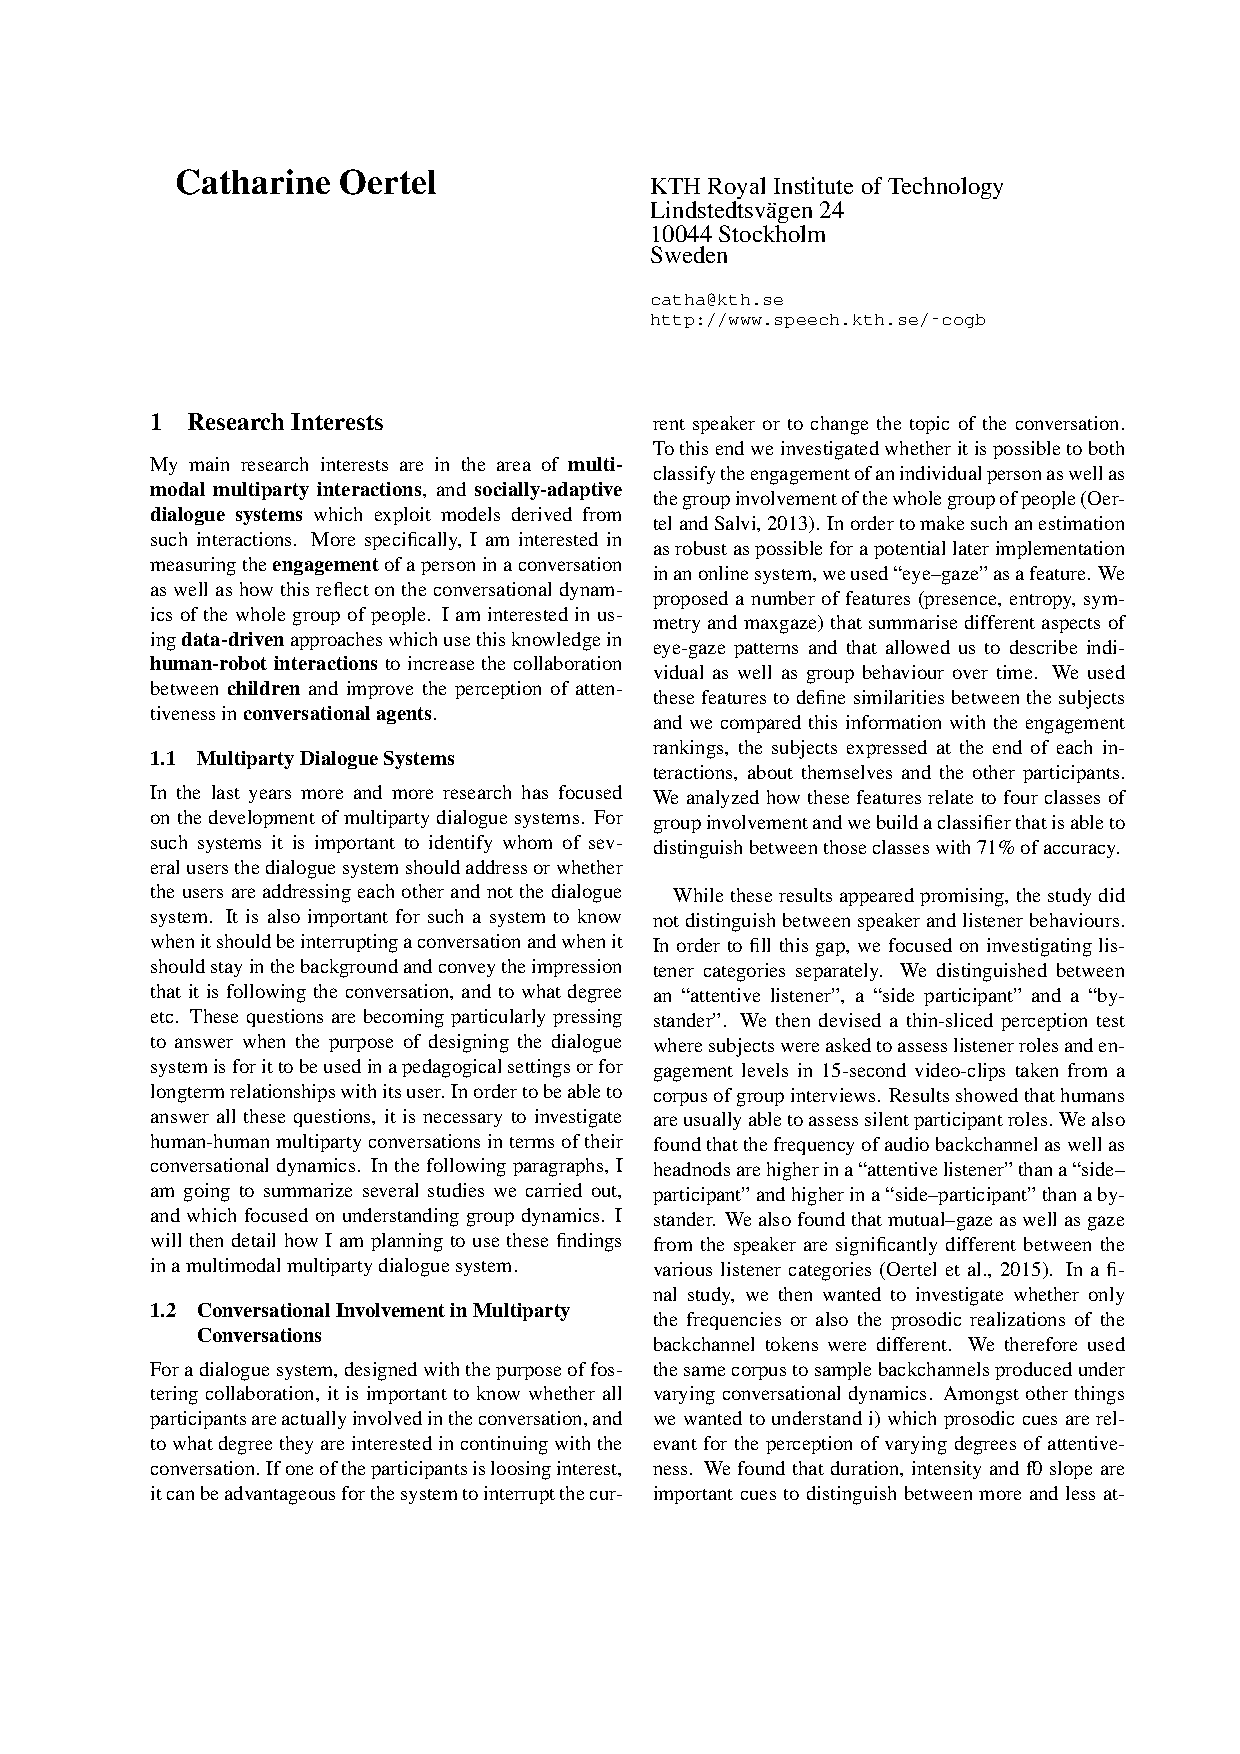
\includepdf[pages=-,pagecommand={},width=\textwidth]{YRRSDS_2016_paper_23_catharine_oertel.pdf}
% 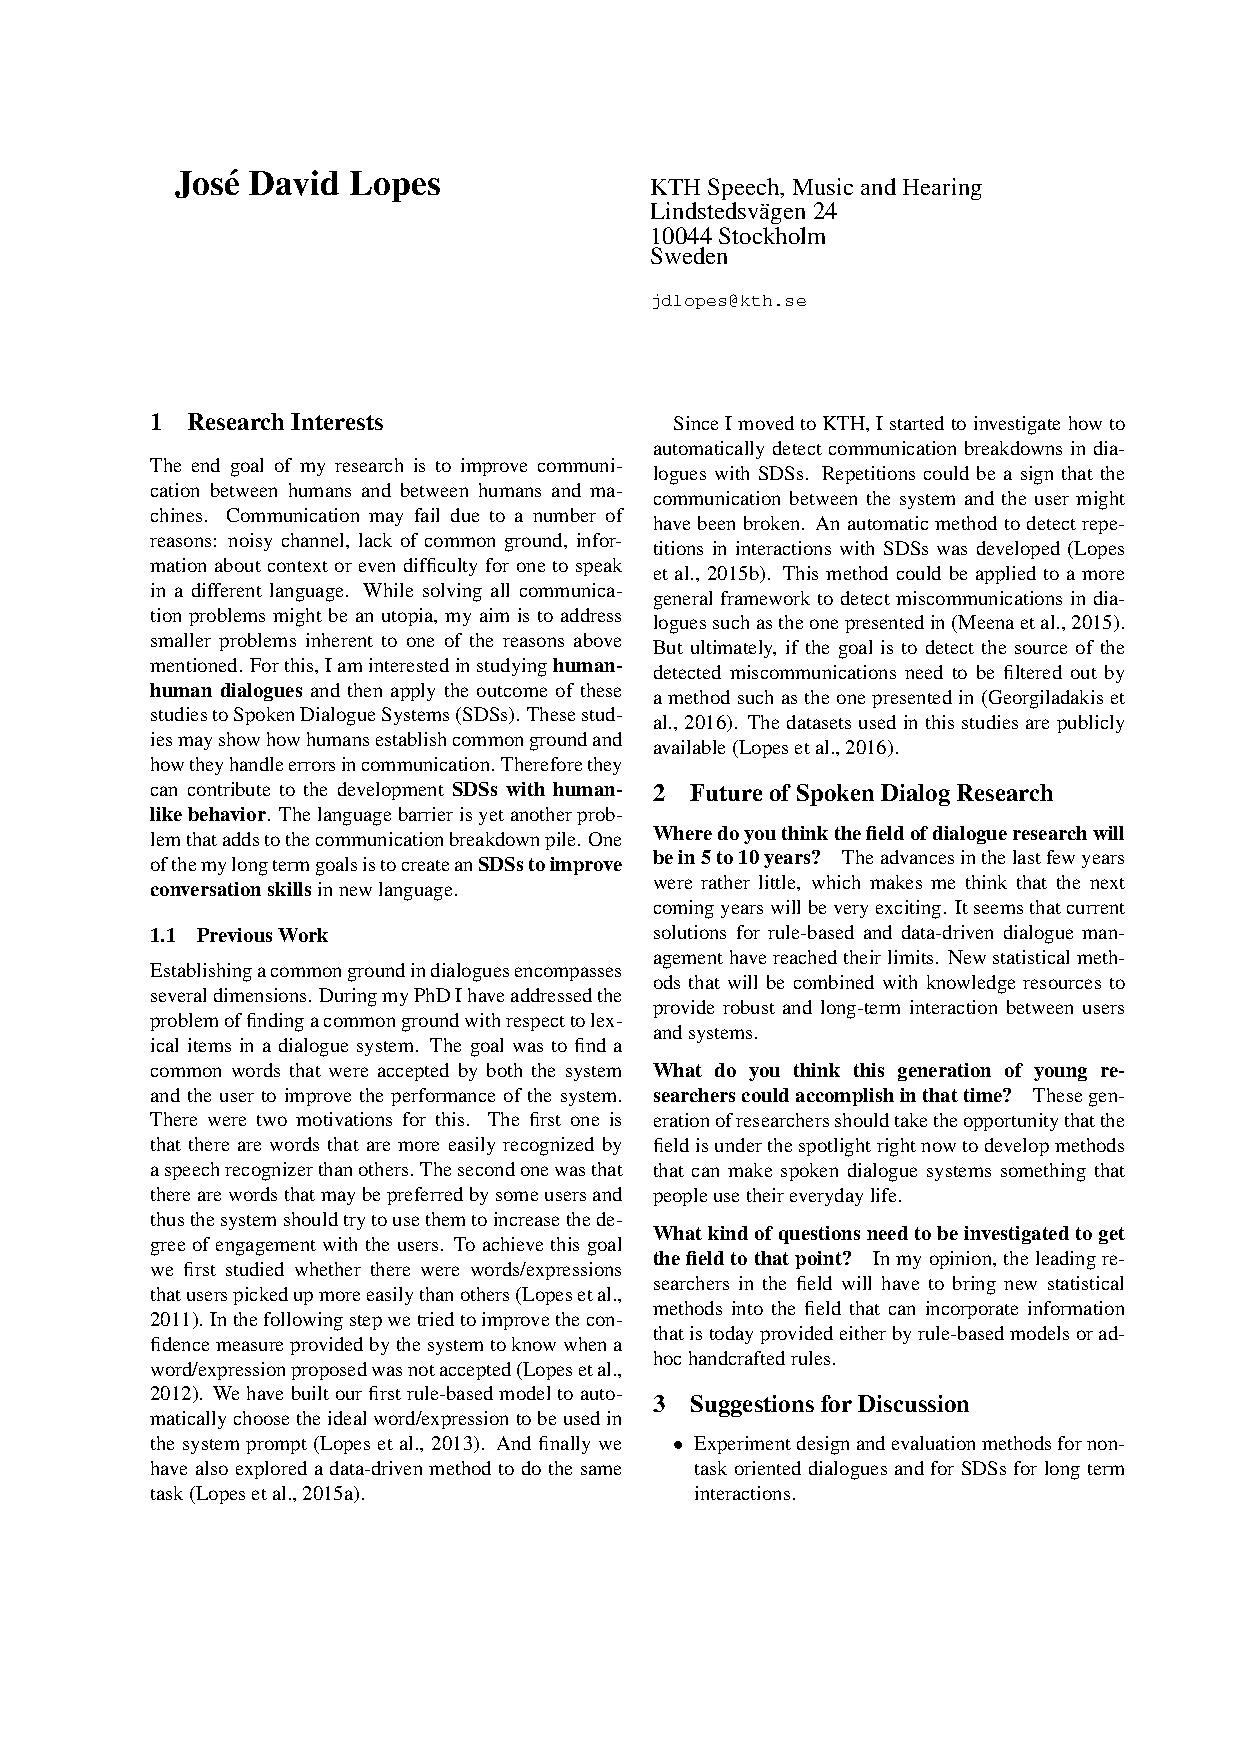
\includepdf[pages=-,pagecommand={},width=\textwidth]{YRRSDS_2016_paper_24_jose_david_lopez.pdf}
% 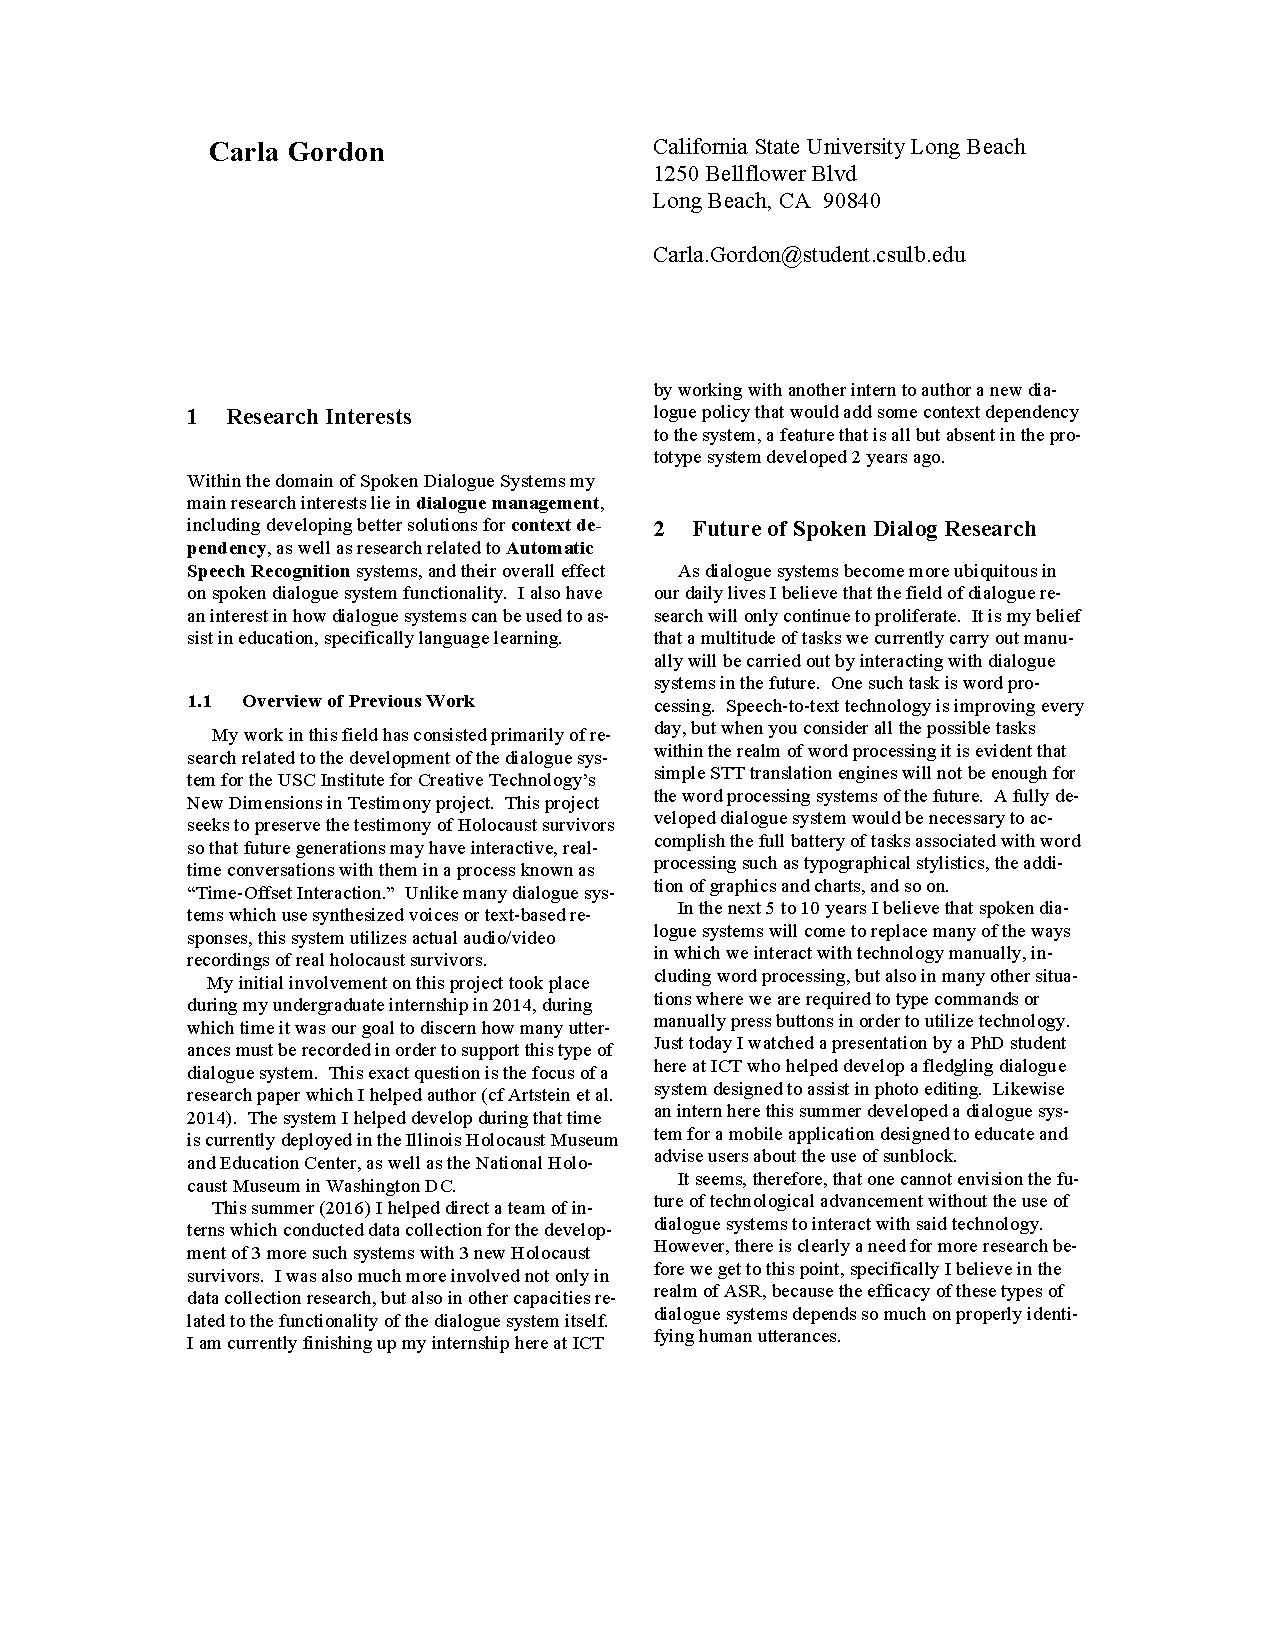
\includepdf[pages=-,pagecommand={},width=\textwidth]{YRRSDS_2016_paper_25_carla_gordon.pdf}
% 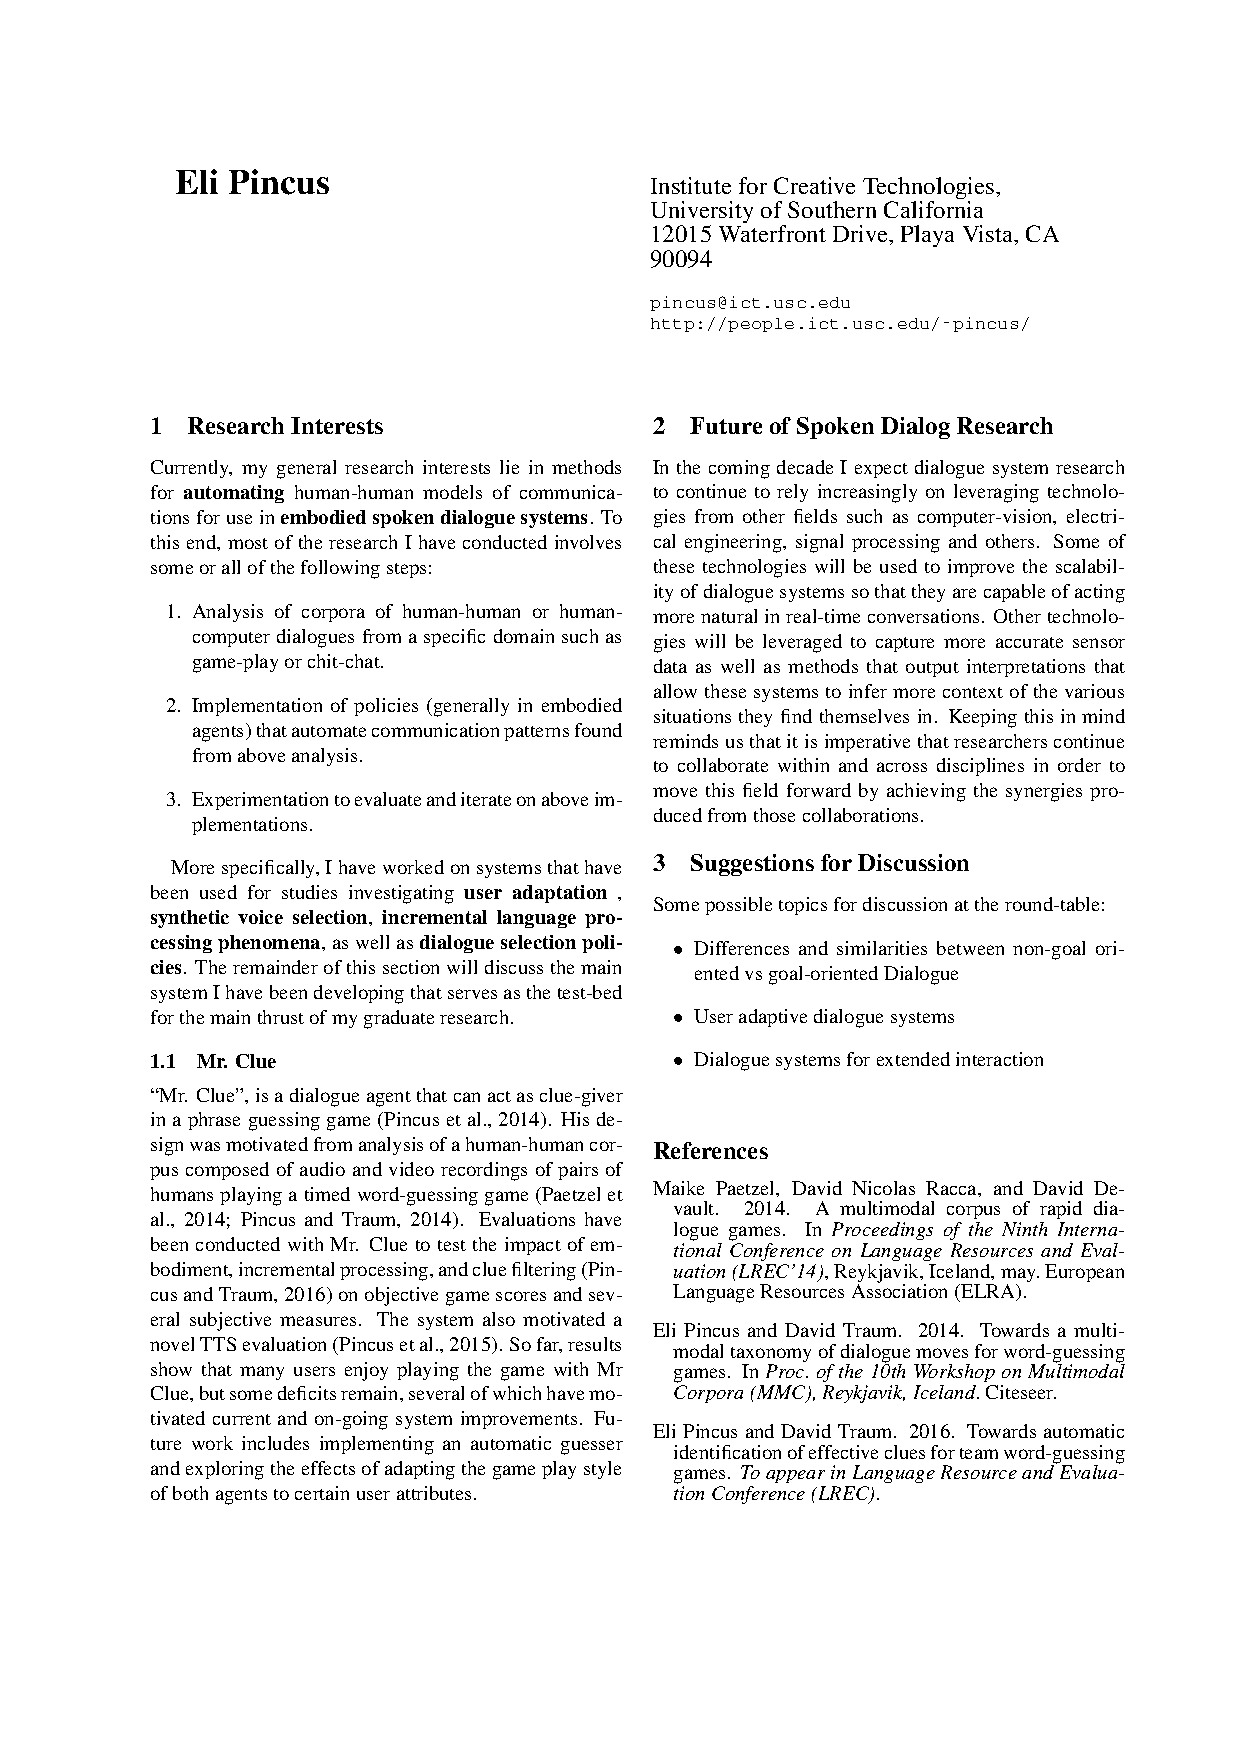
\includepdf[pages=-,pagecommand={},width=\textwidth]{YRRSDS_2016_paper_26_eli_pincus.pdf}



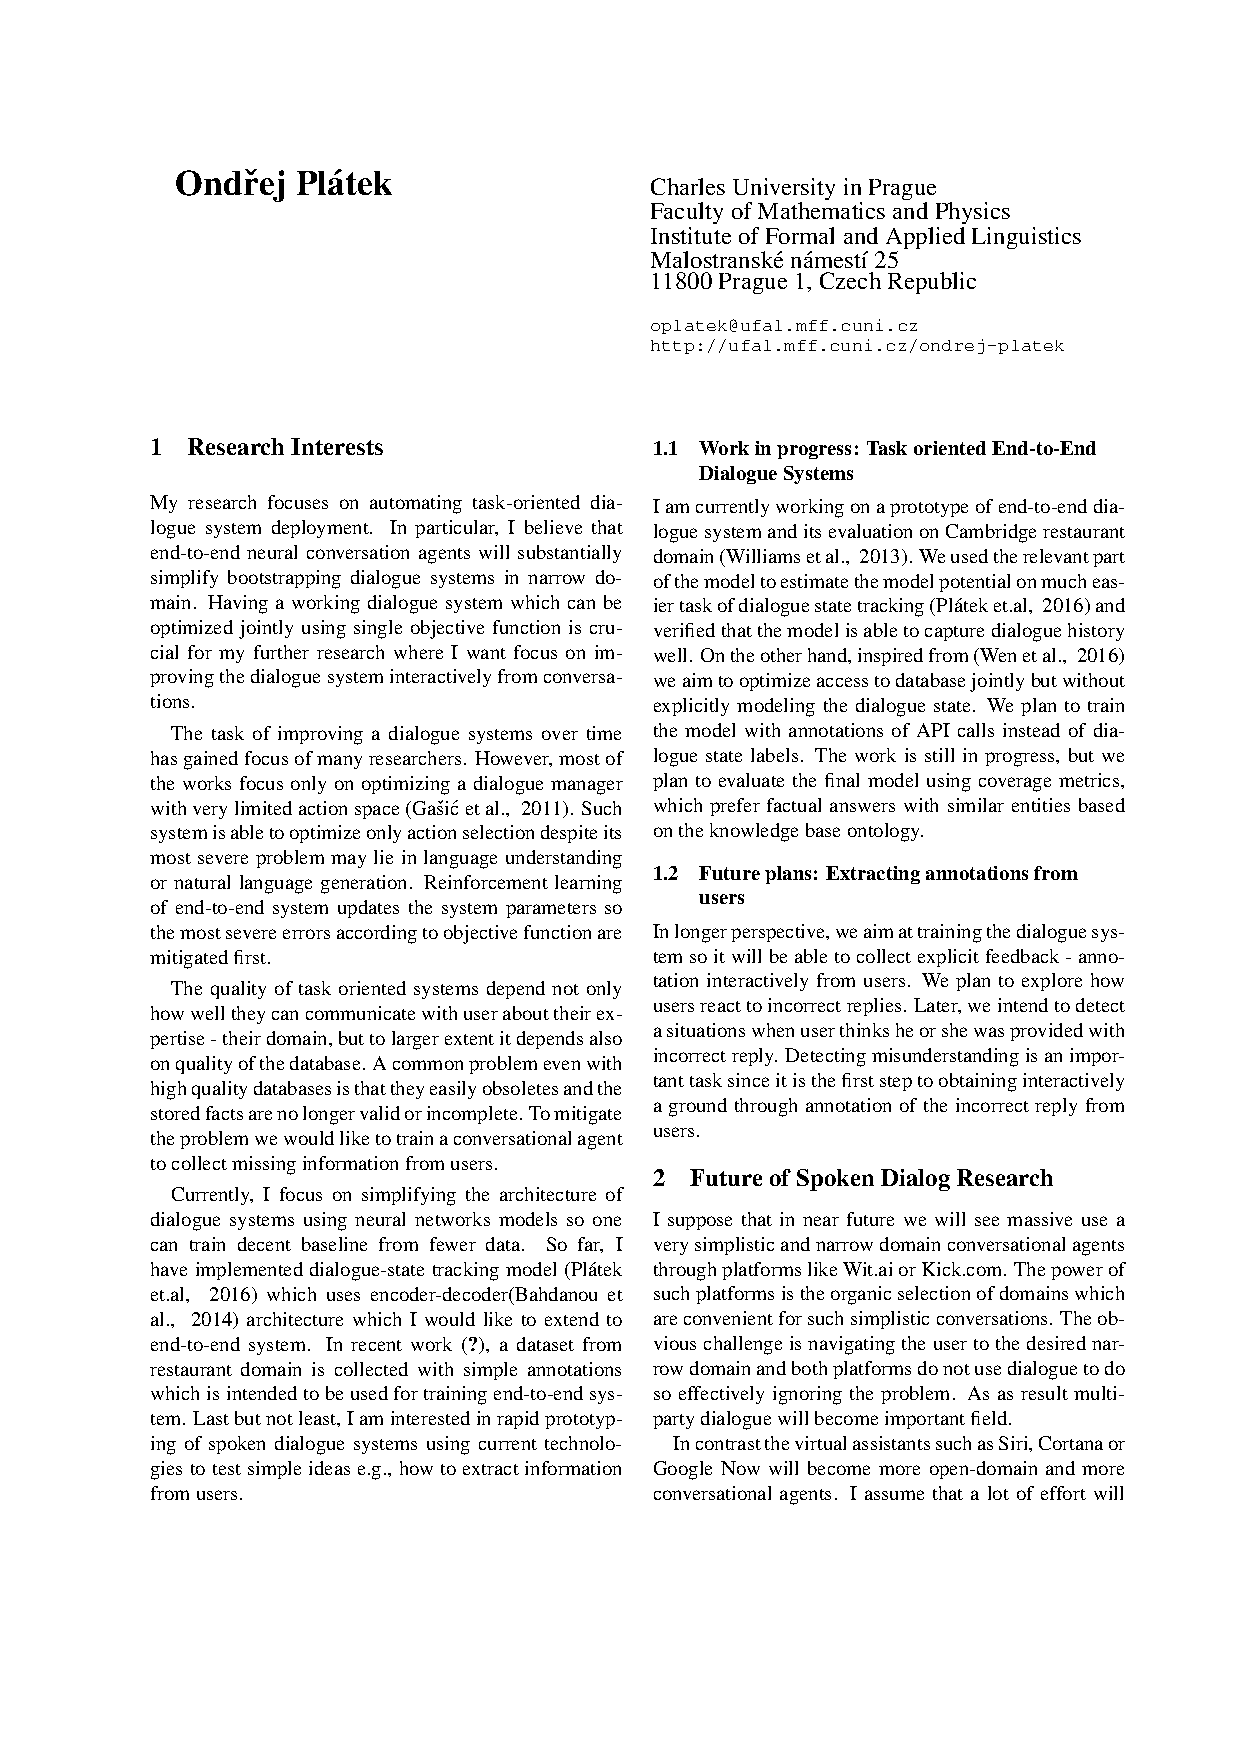
\includepdf[pages=-,pagecommand={}]{YRRSDS_2016_paper_1_ondrej_platek.pdf}
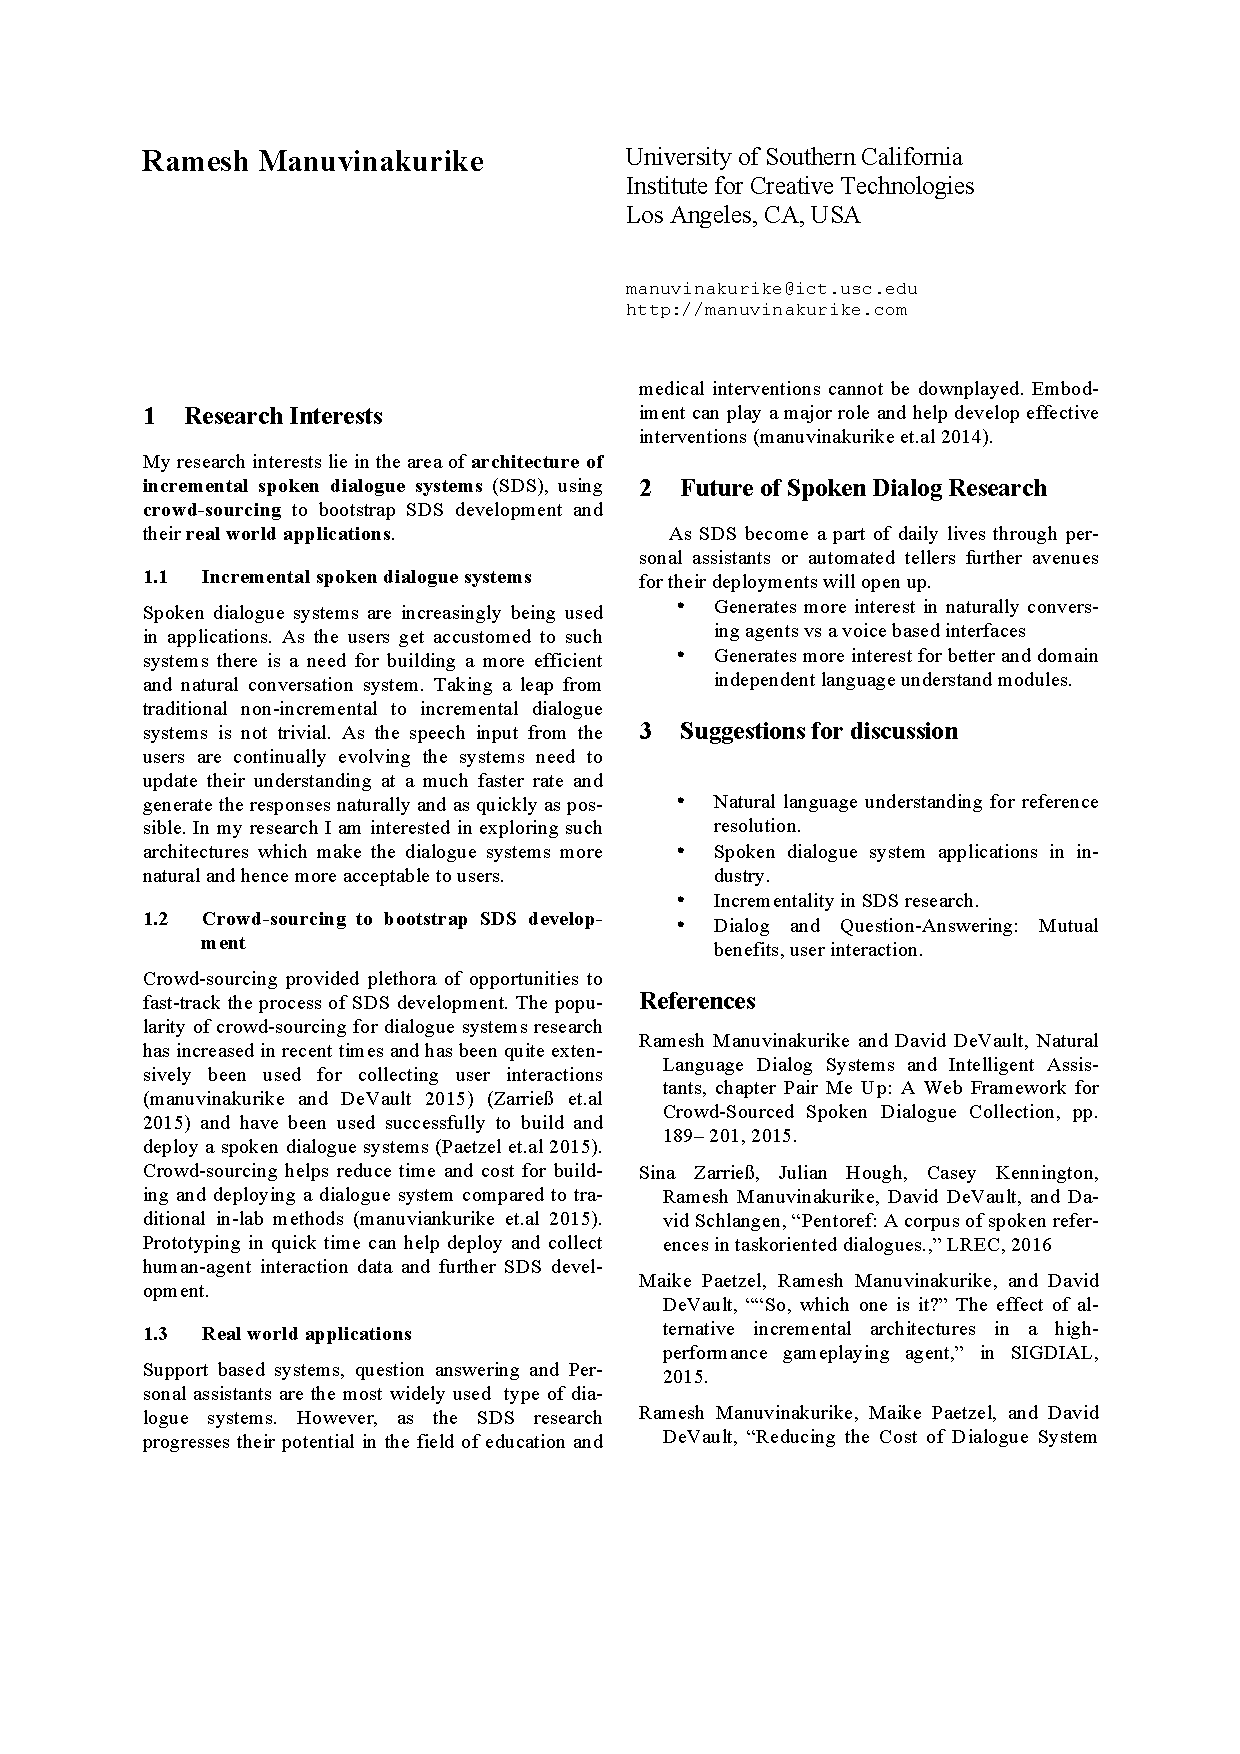
\includepdf[pages=-,pagecommand={}]{YRRSDS_2016_paper_2_remesh_manuvinakurike.pdf}
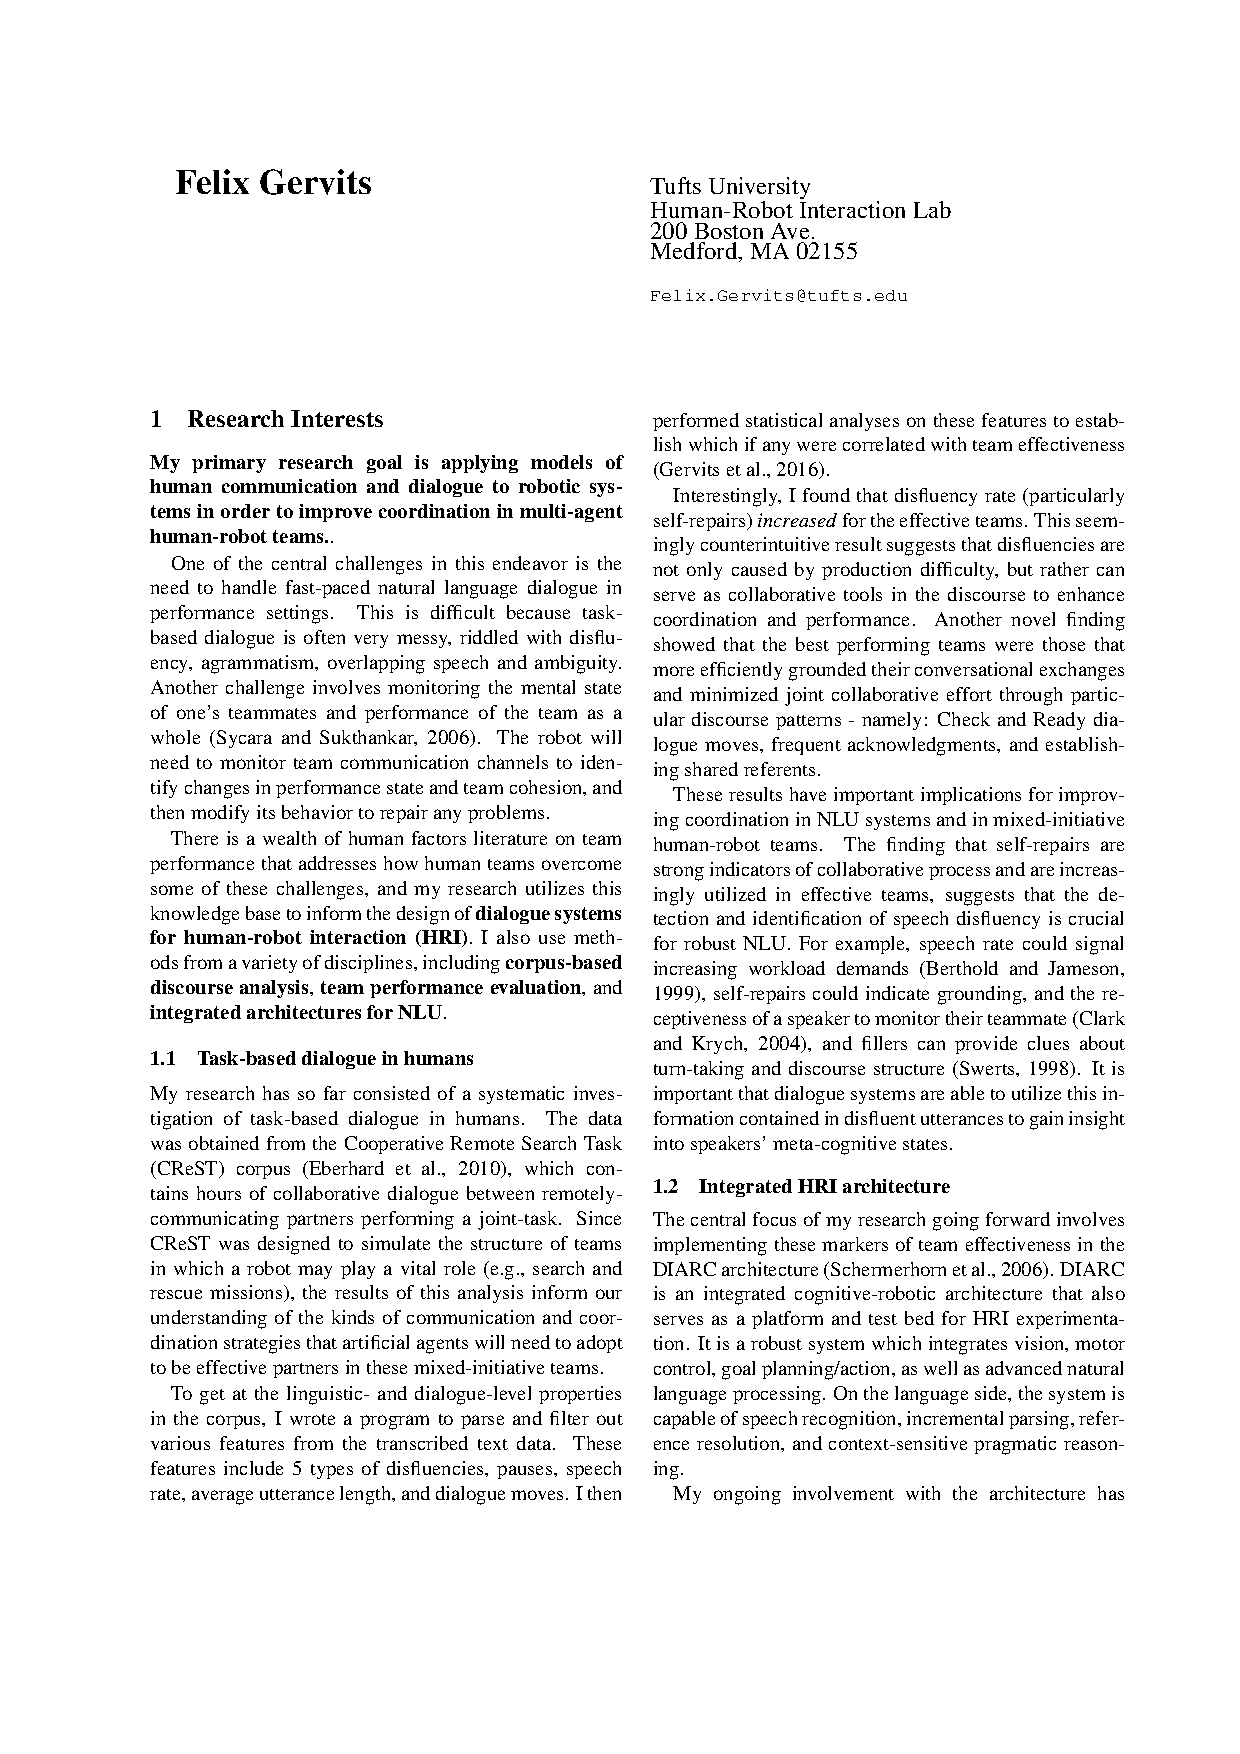
\includepdf[pages=-,pagecommand={}]{YRRSDS_2016_paper_3_felix_gervits.pdf}
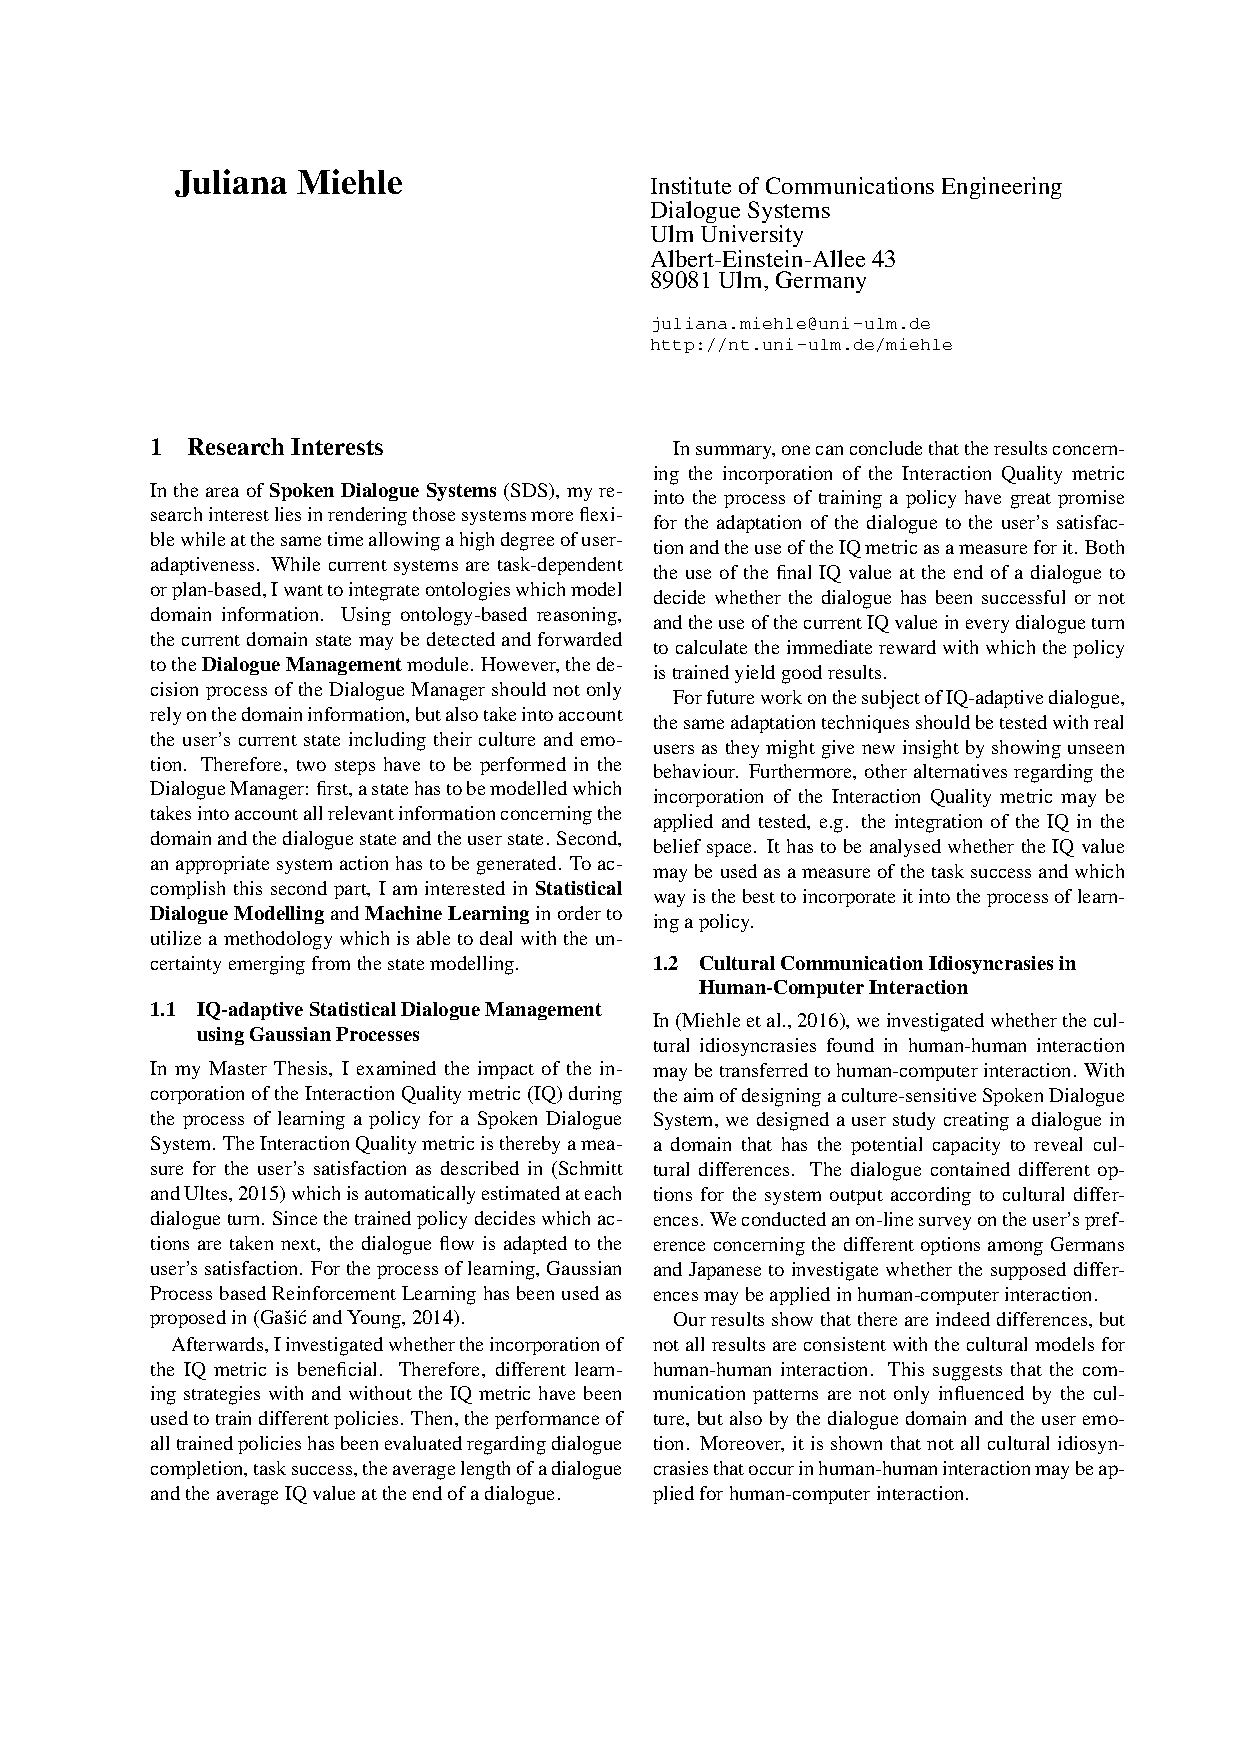
\includepdf[pages=-,pagecommand={}]{YRRSDS_2016_paper_4_juliana_miehle.pdf}
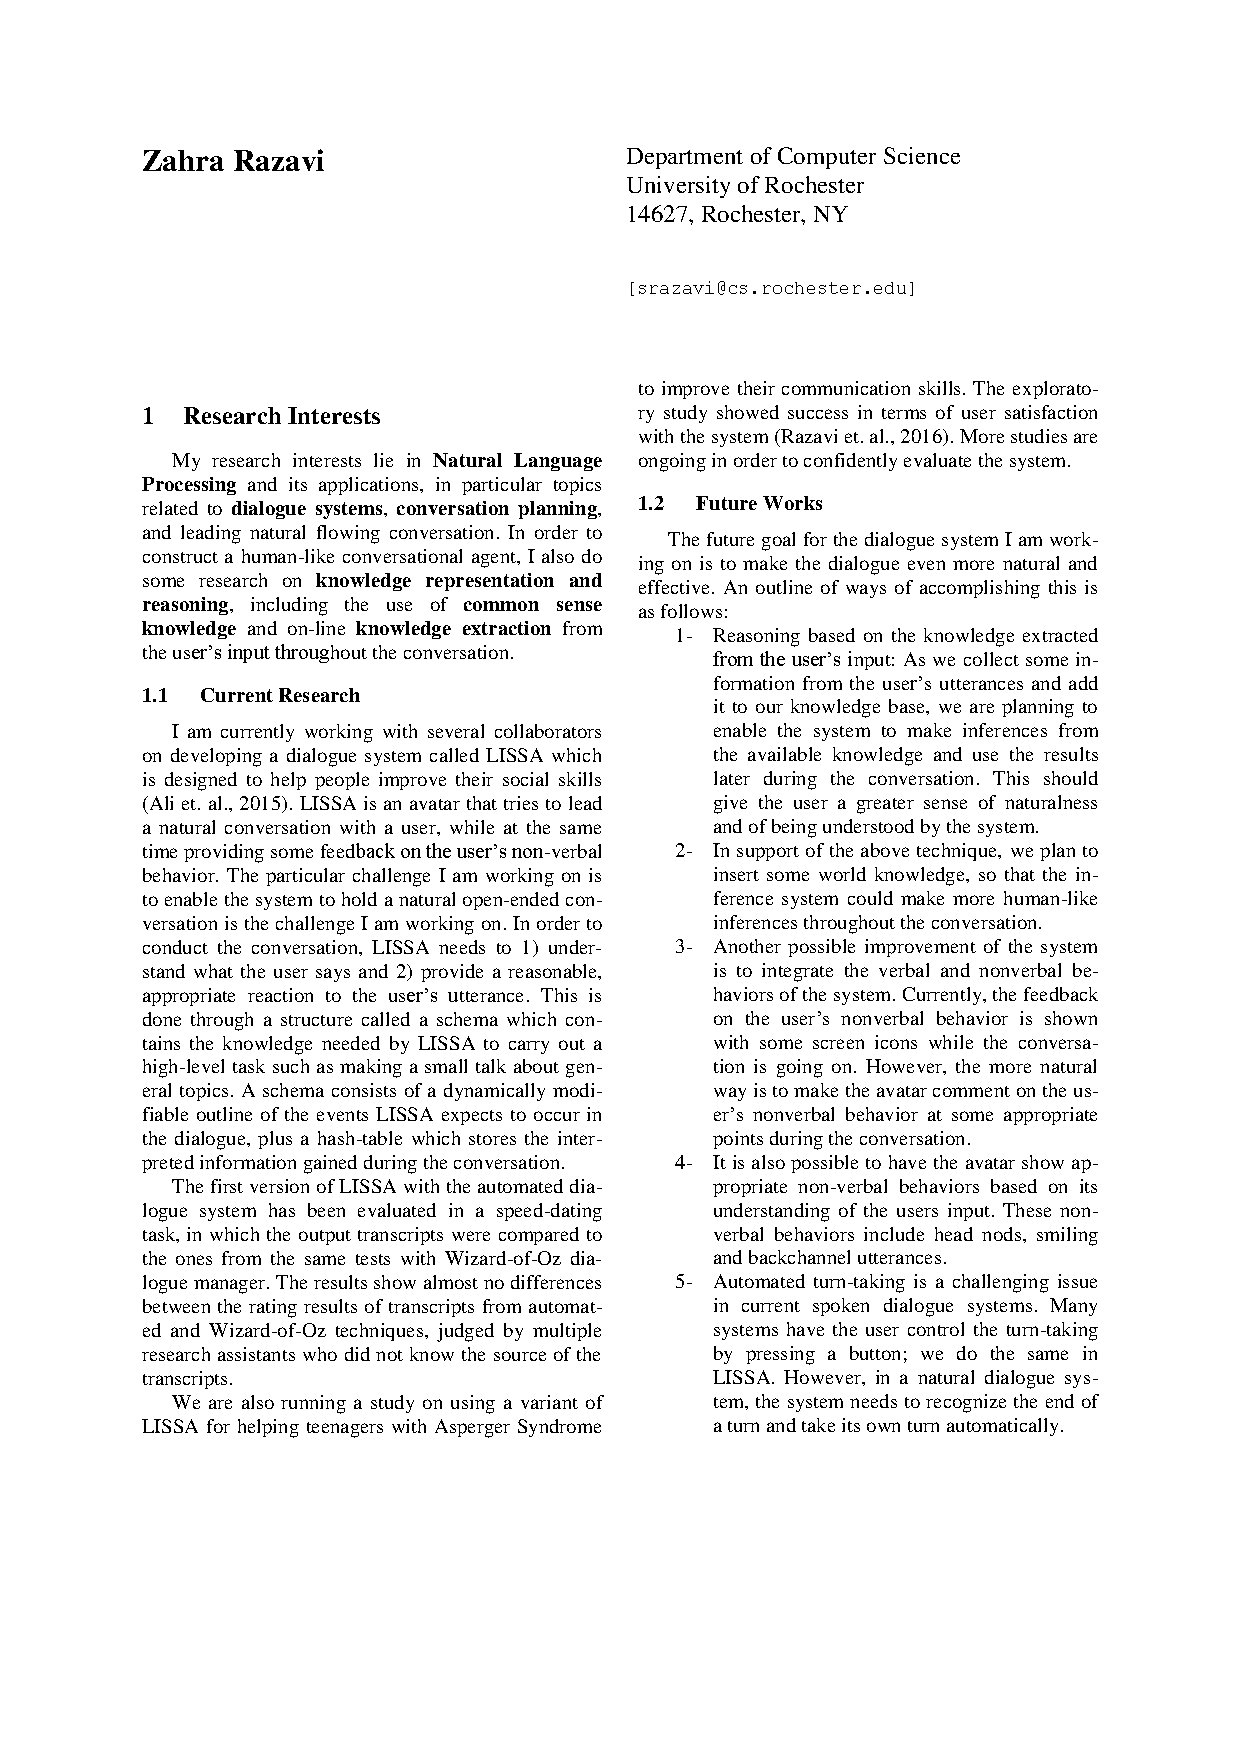
\includepdf[pages=-,pagecommand={}]{YRRSDS_2016_paper_5_zahra_razavi.pdf}
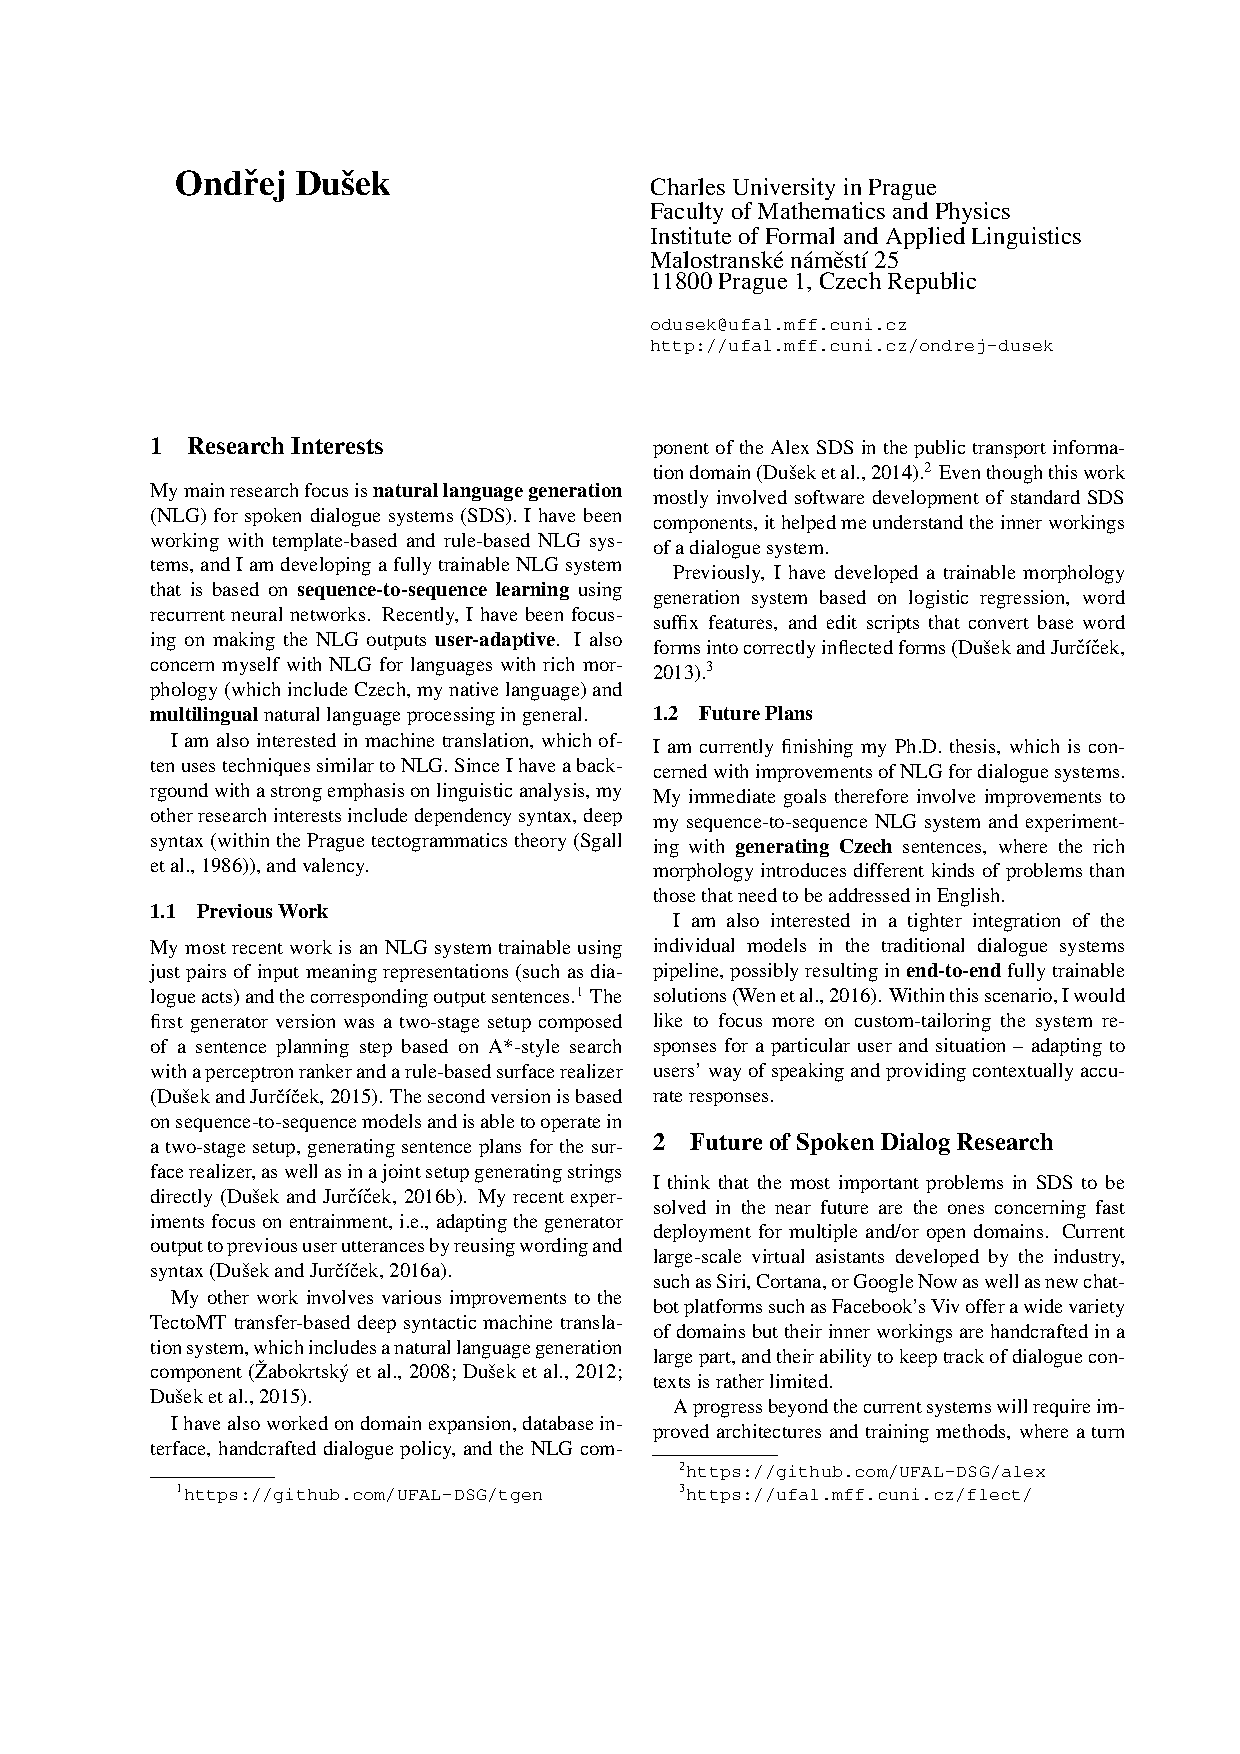
\includepdf[pages=-,pagecommand={}]{YRRSDS_2016_paper_6_ondrej_dusek.pdf}
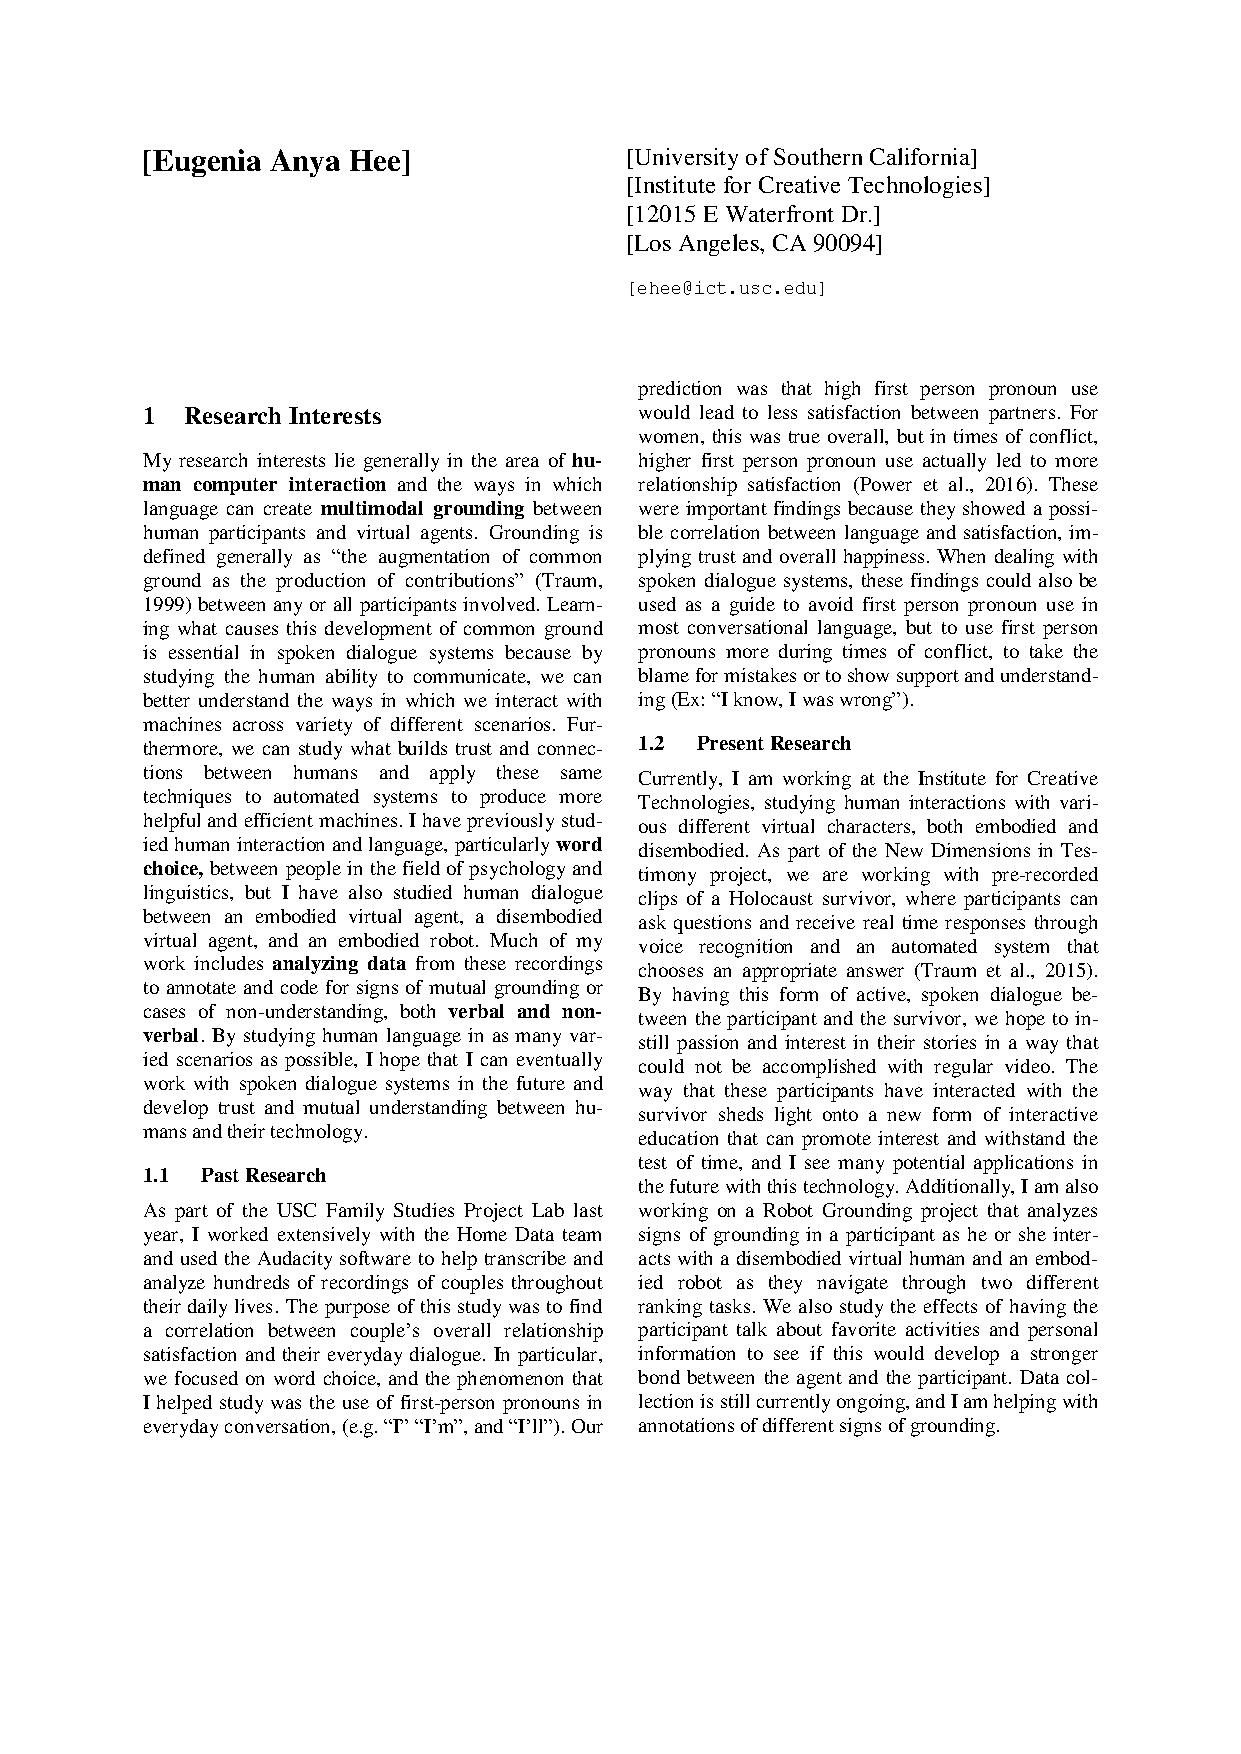
\includepdf[pages=-,pagecommand={}]{YRRSDS_2016_paper_7_eugenia_hee.pdf}
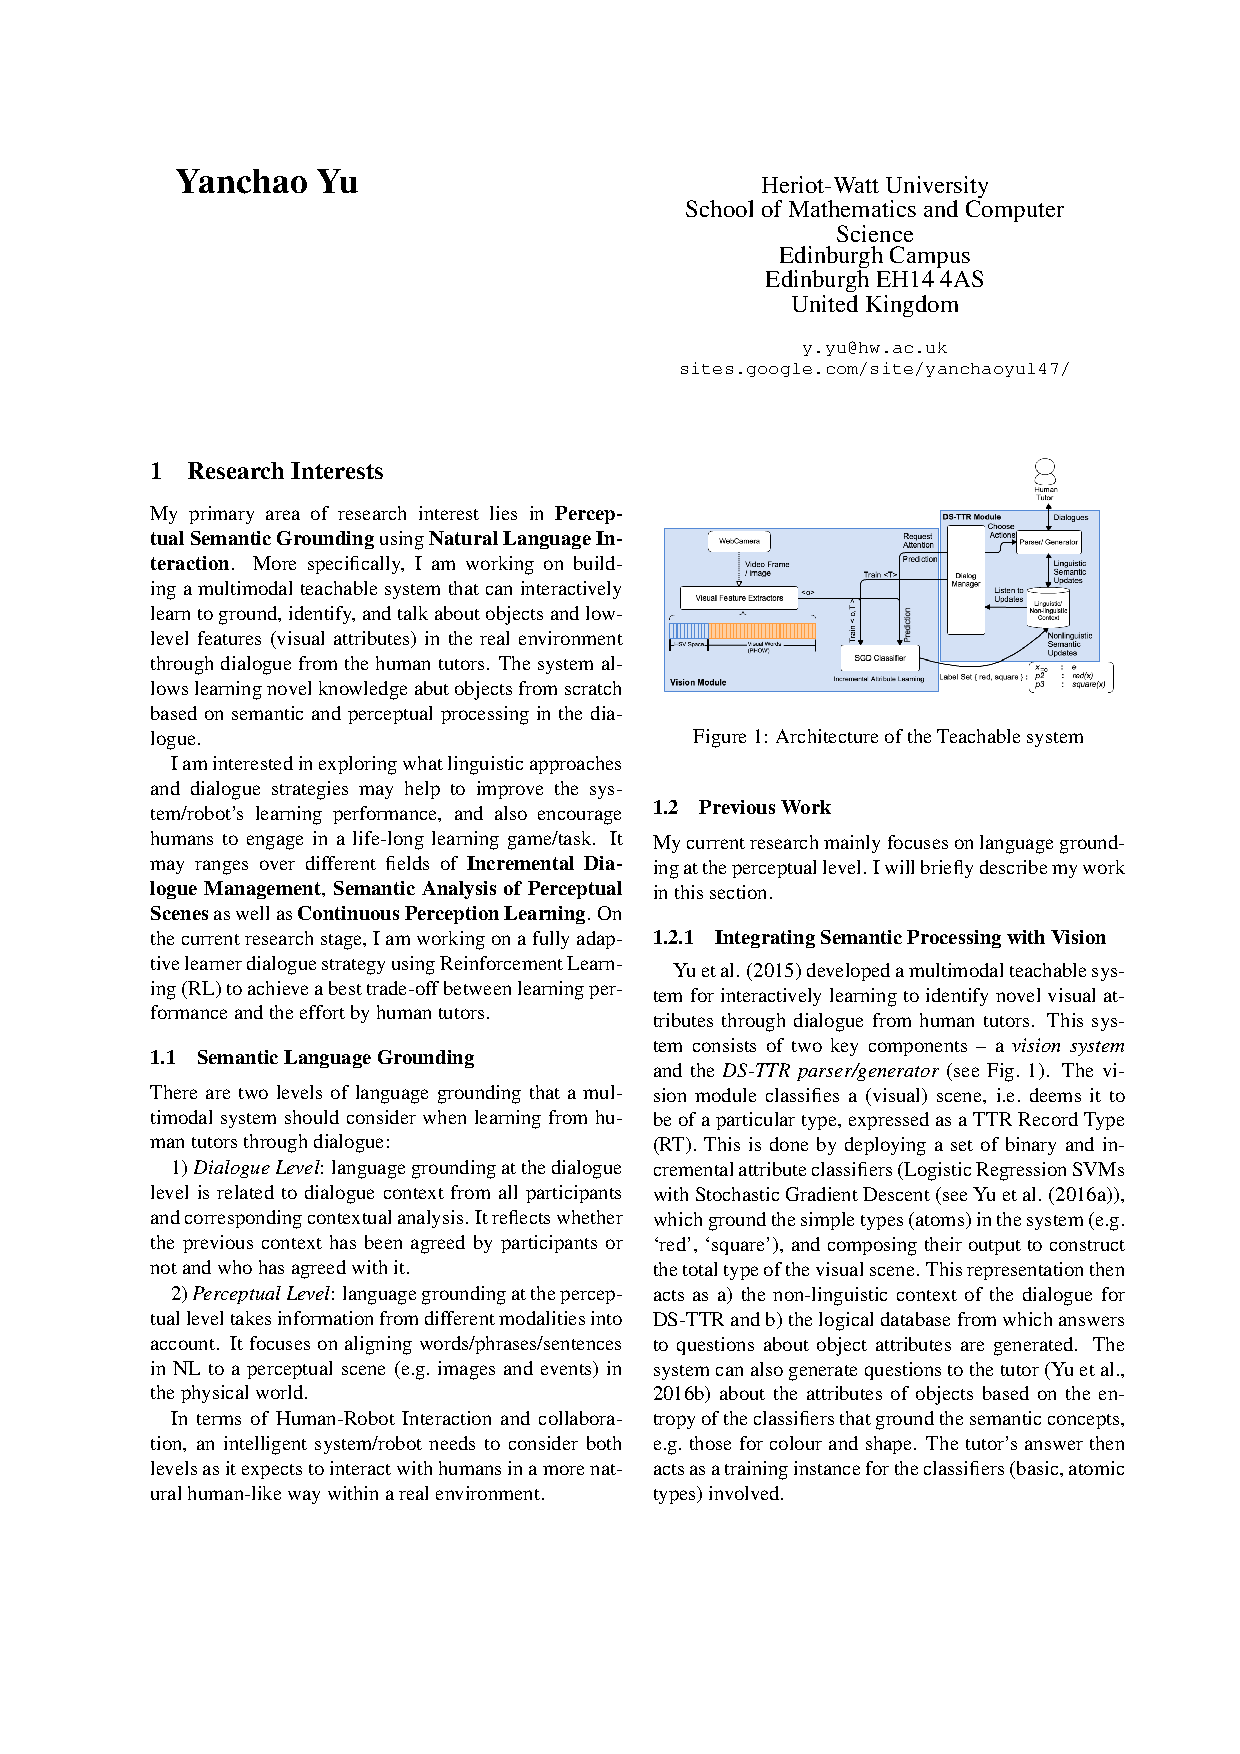
\includepdf[pages=-,pagecommand={}]{YRRSDS_2016_paper_8_uanchao_yu.pdf}
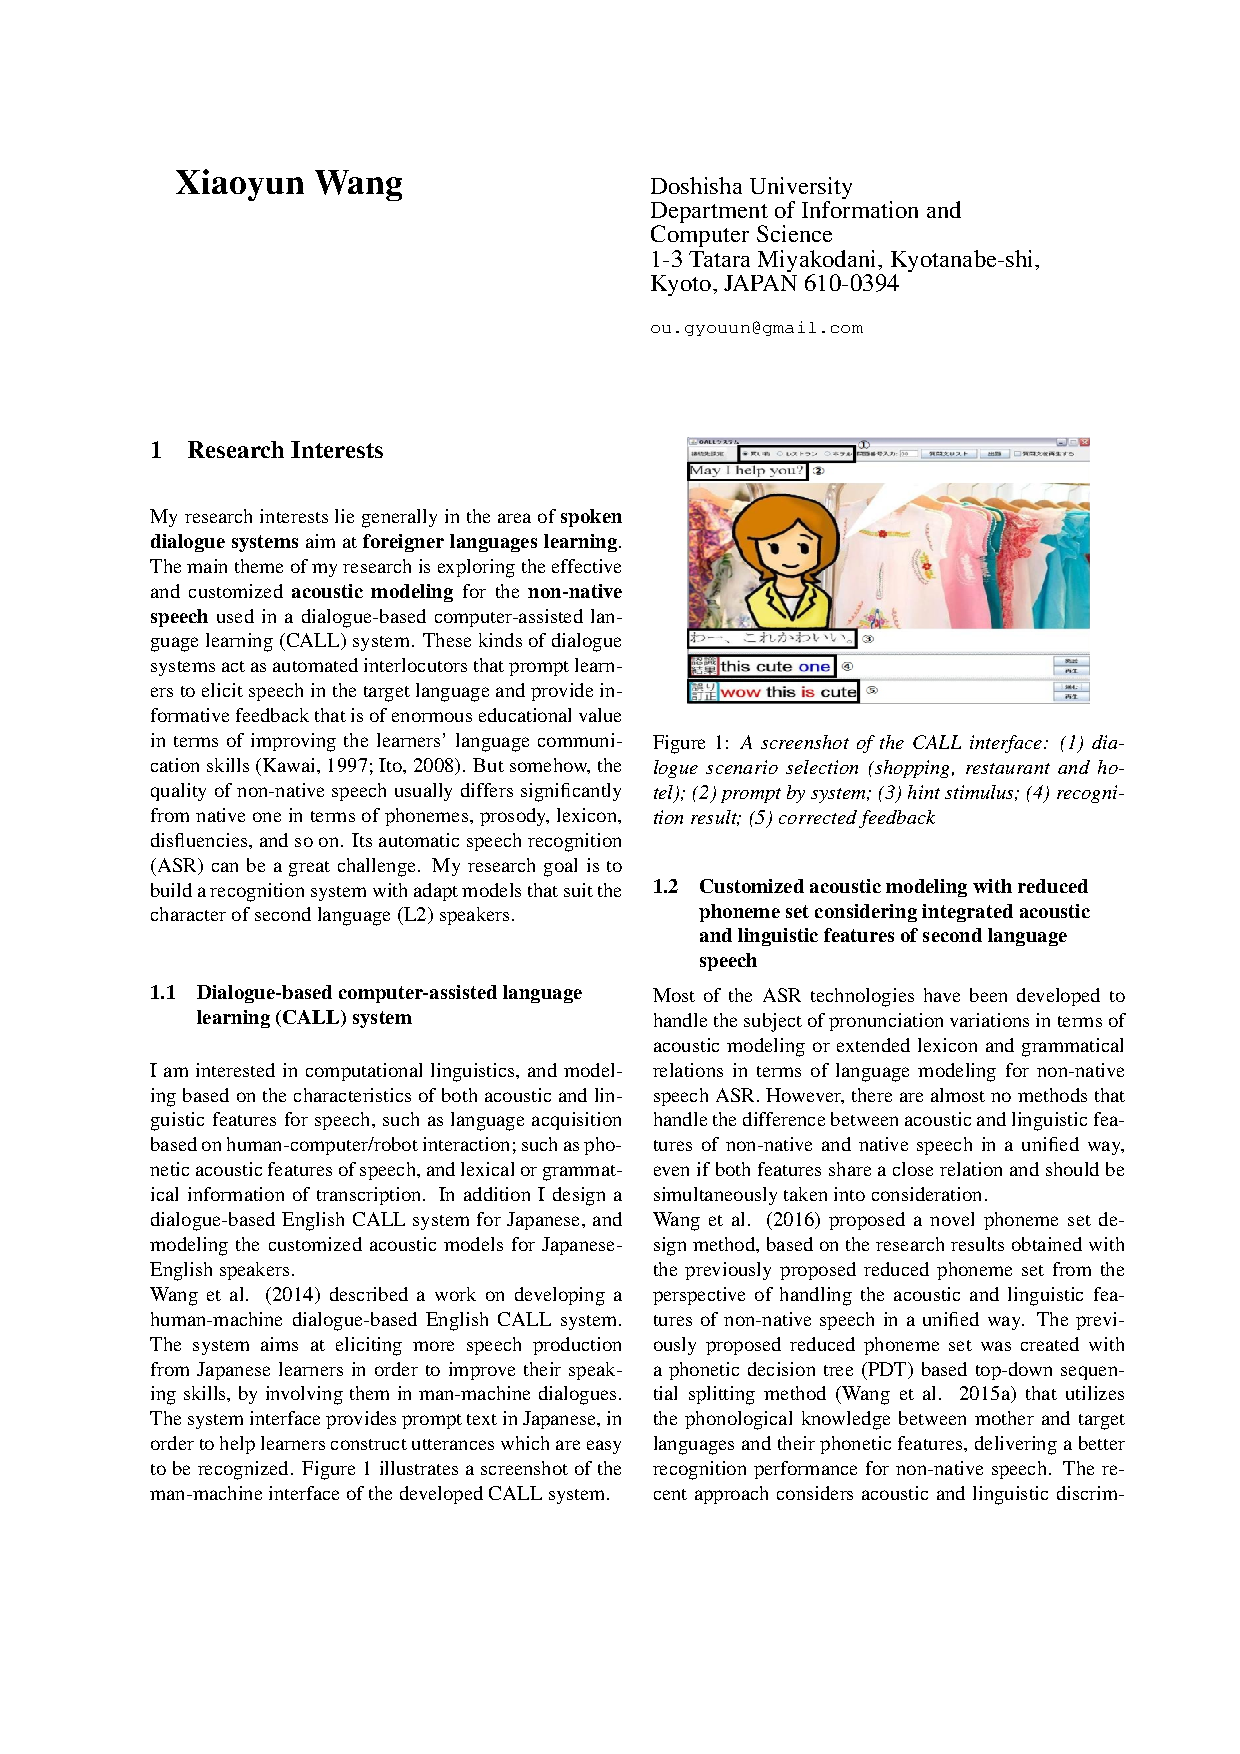
\includepdf[pages=-,pagecommand={}]{YRRSDS_2016_paper_9_xiaoyun_wang.pdf}
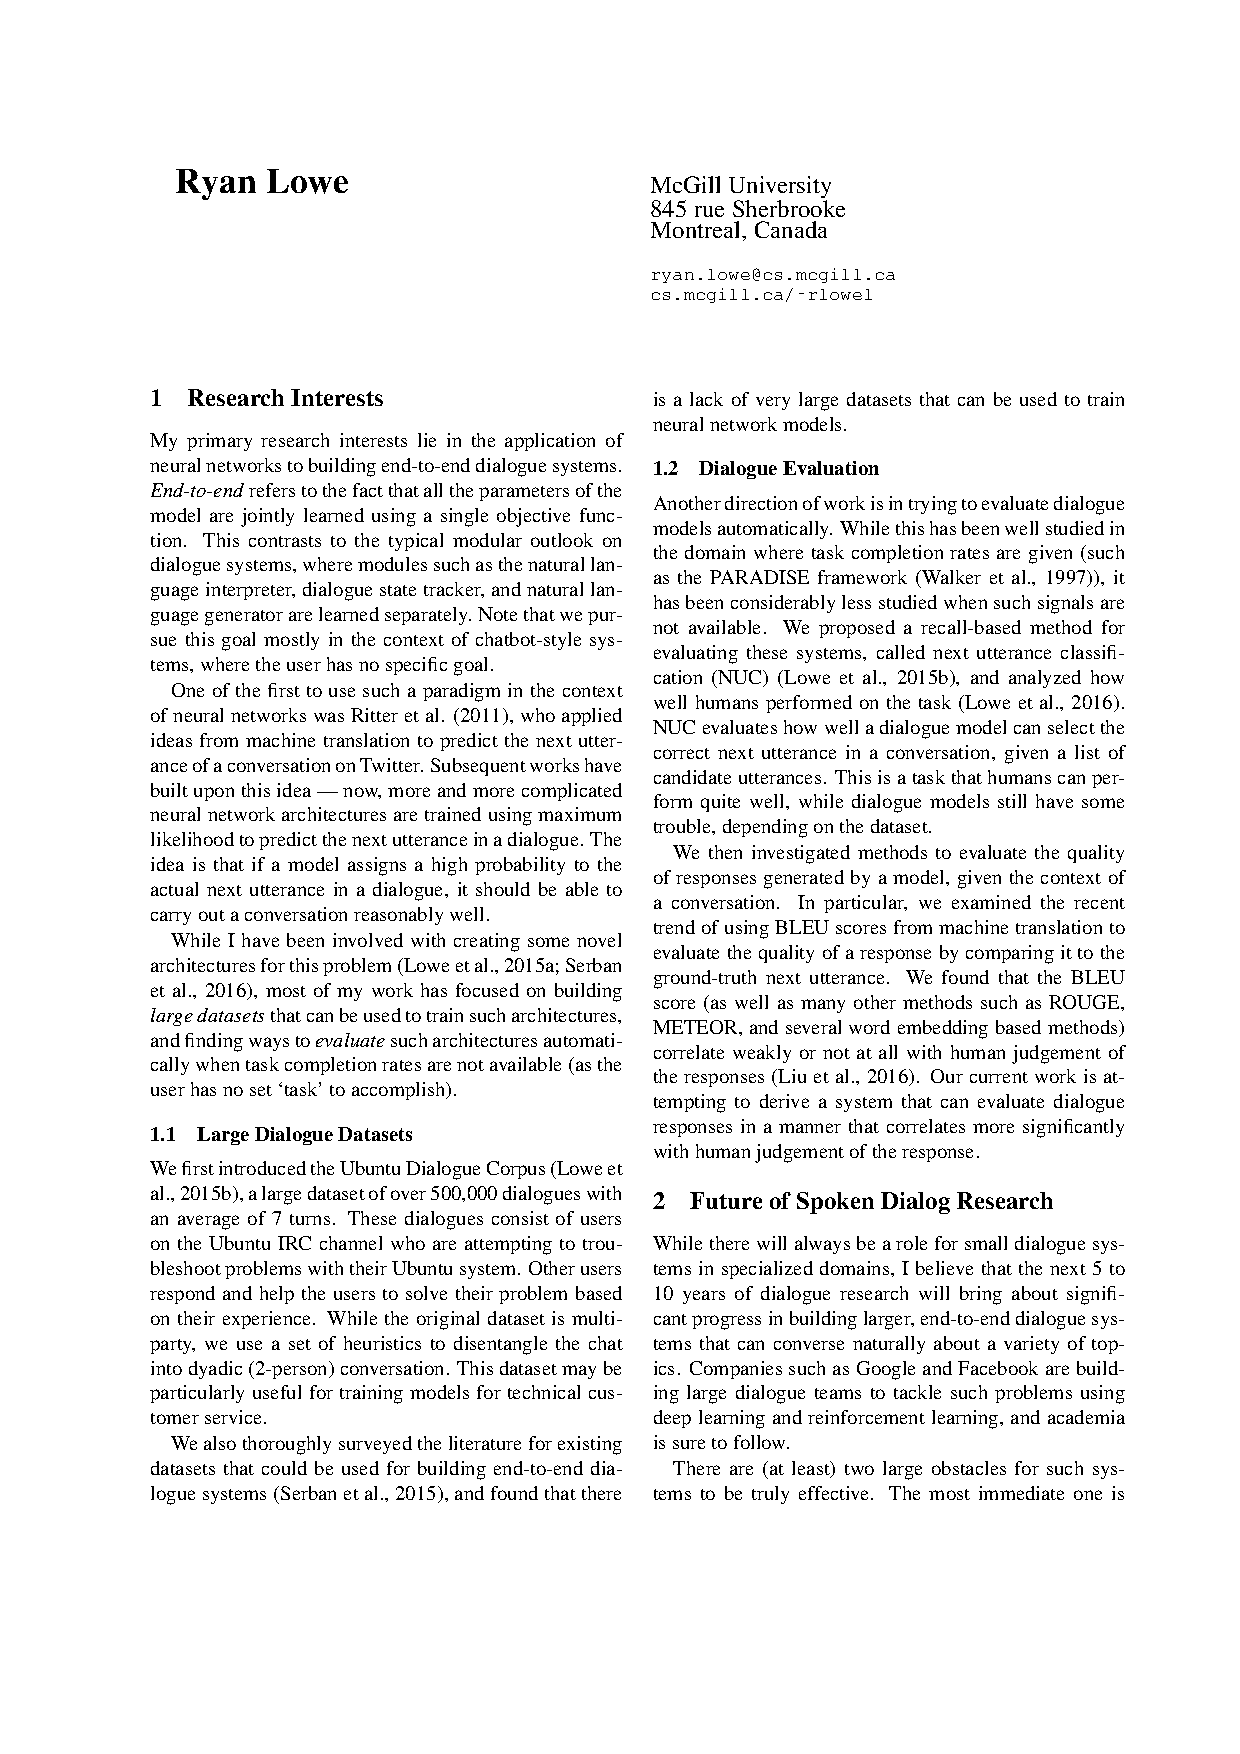
\includepdf[pages=-,pagecommand={}]{YRRSDS_2016_paper_10_rayn_lowe.pdf}
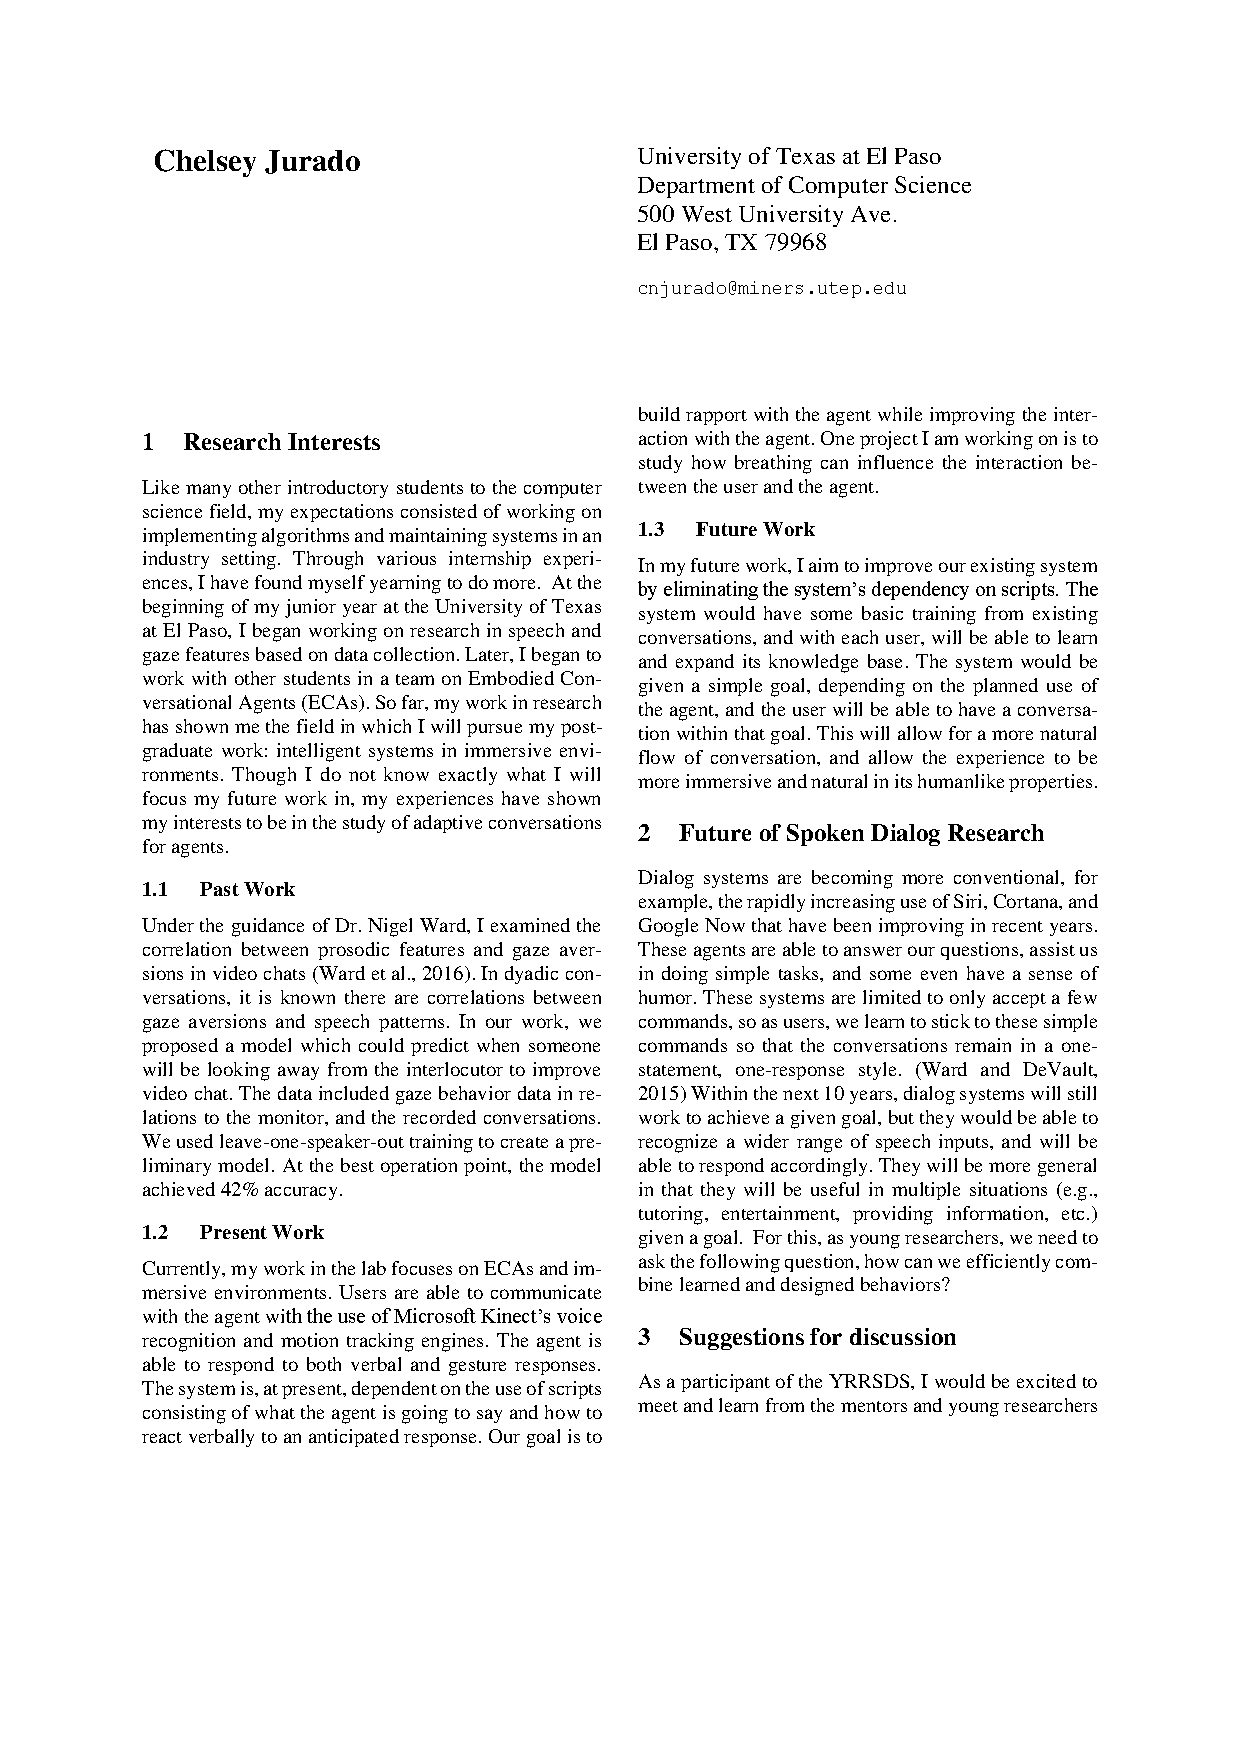
\includepdf[pages=-,pagecommand={}]{YRRSDS_2016_paper_11_chelsey_jurado.pdf}
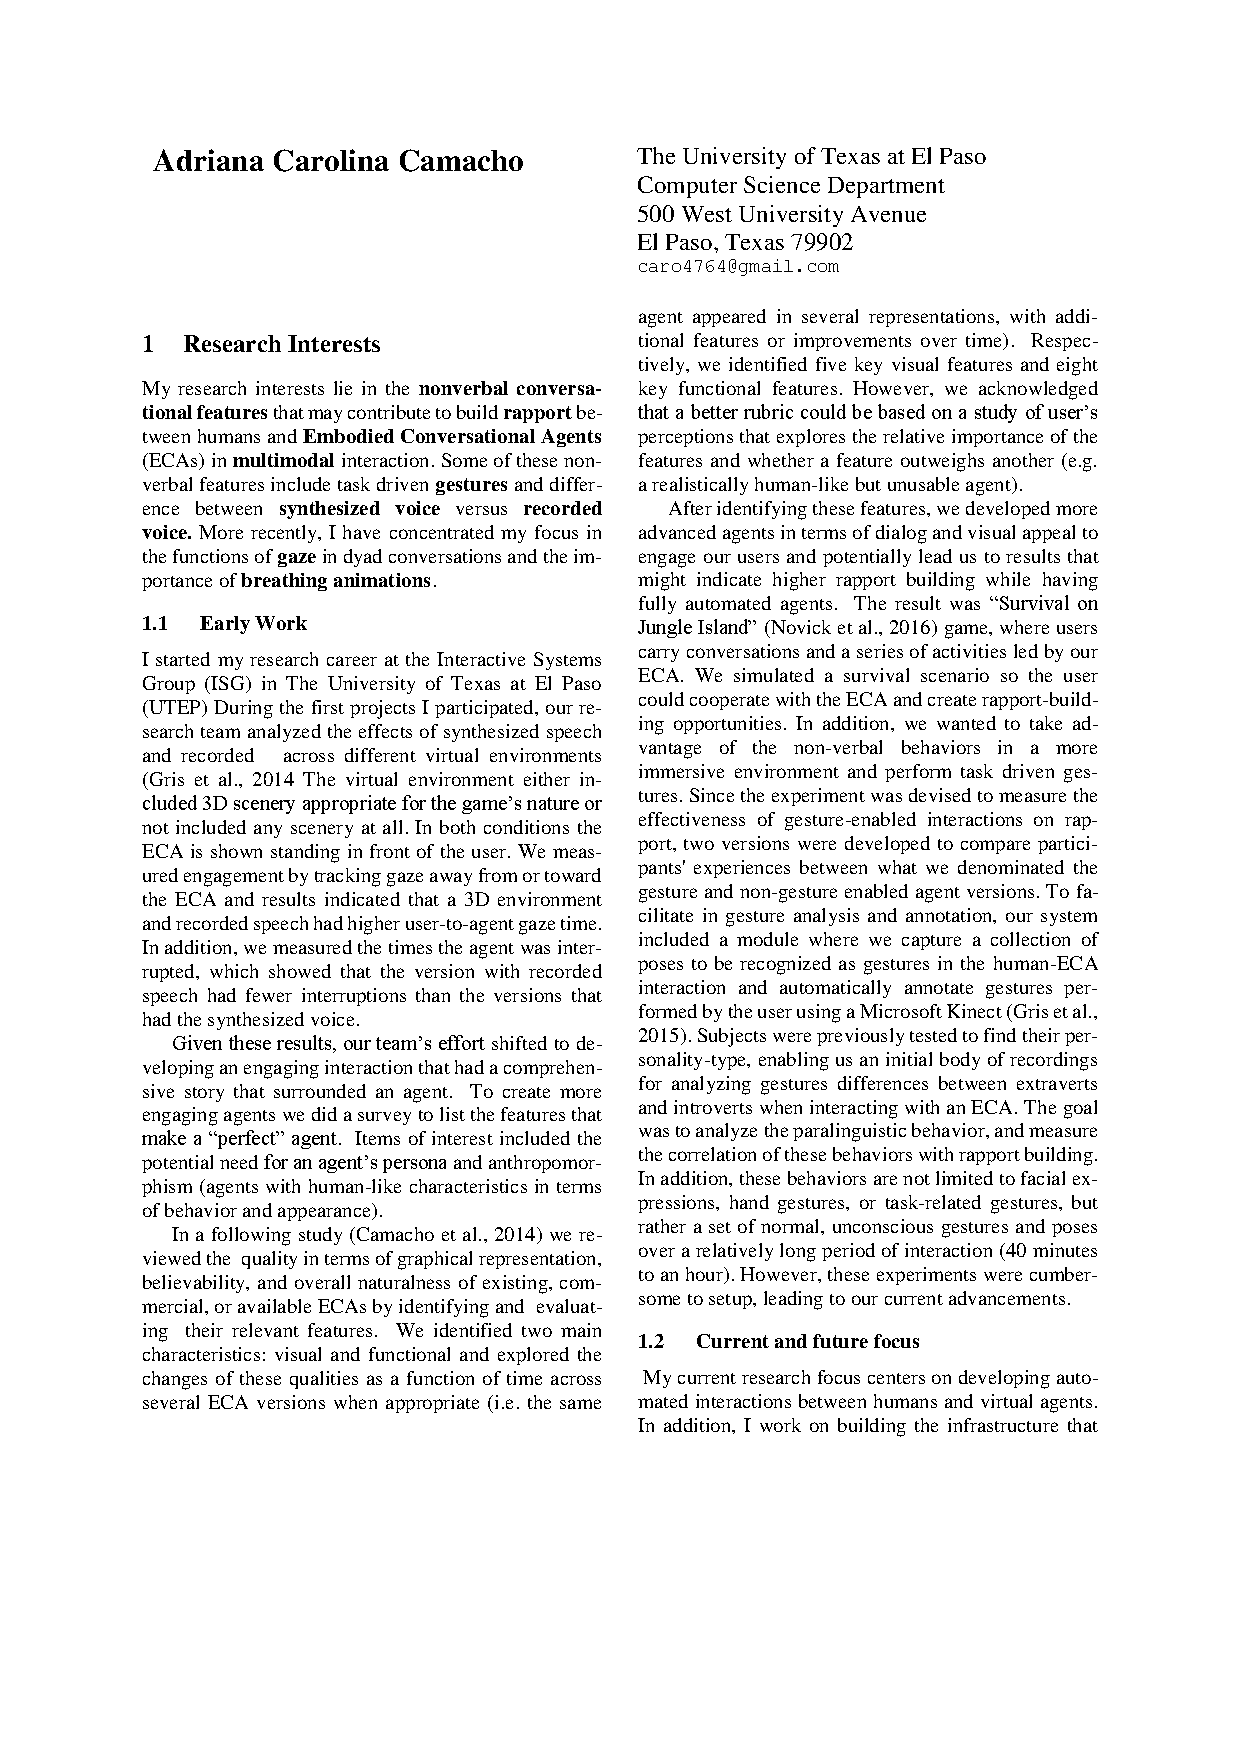
\includepdf[pages=-,pagecommand={}]{YRRSDS_2016_paper_12_adriana_camacho.pdf}
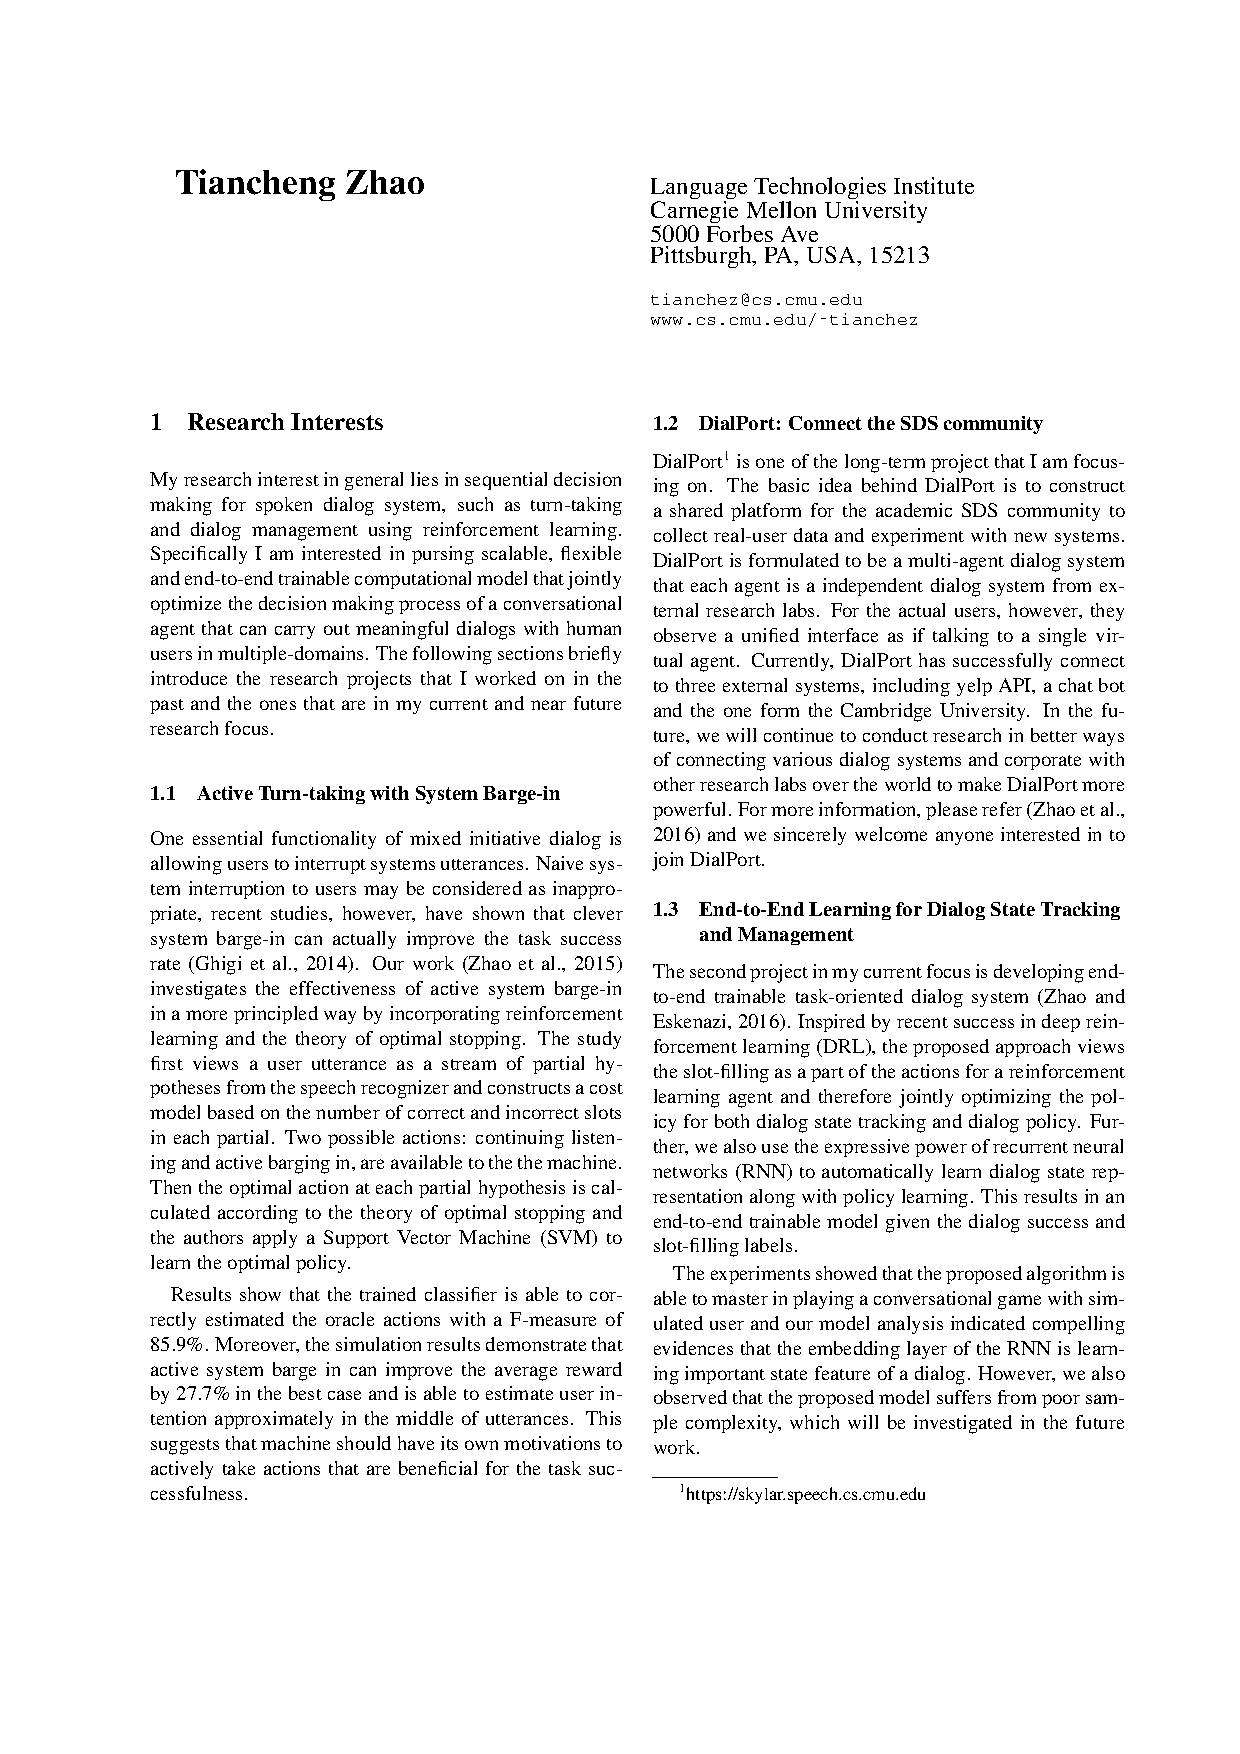
\includepdf[pages=-,pagecommand={}]{YRRSDS_2016_paper_14_tiancheng_zhao.pdf}
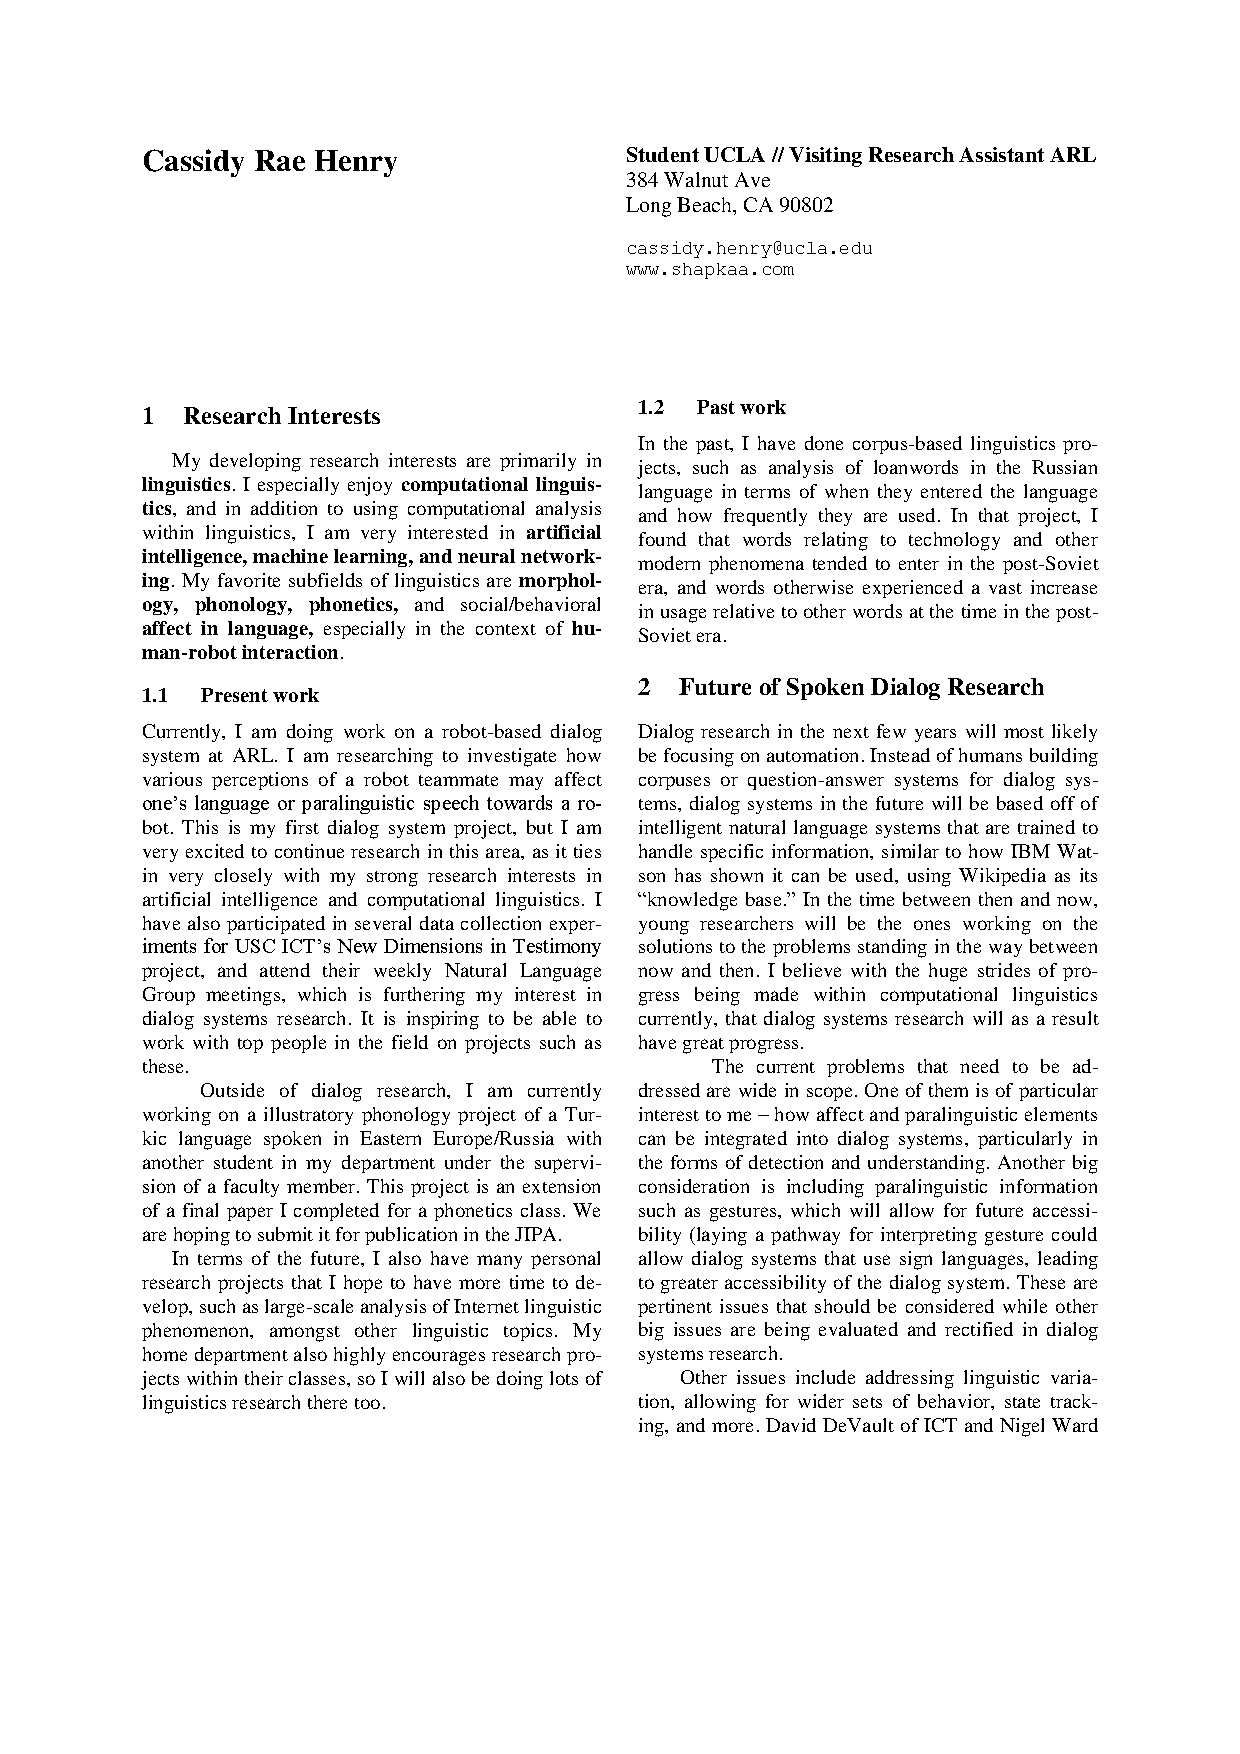
\includepdf[pages=-,pagecommand={}]{YRRSDS_2016_paper_15_cassidy_henry.pdf}
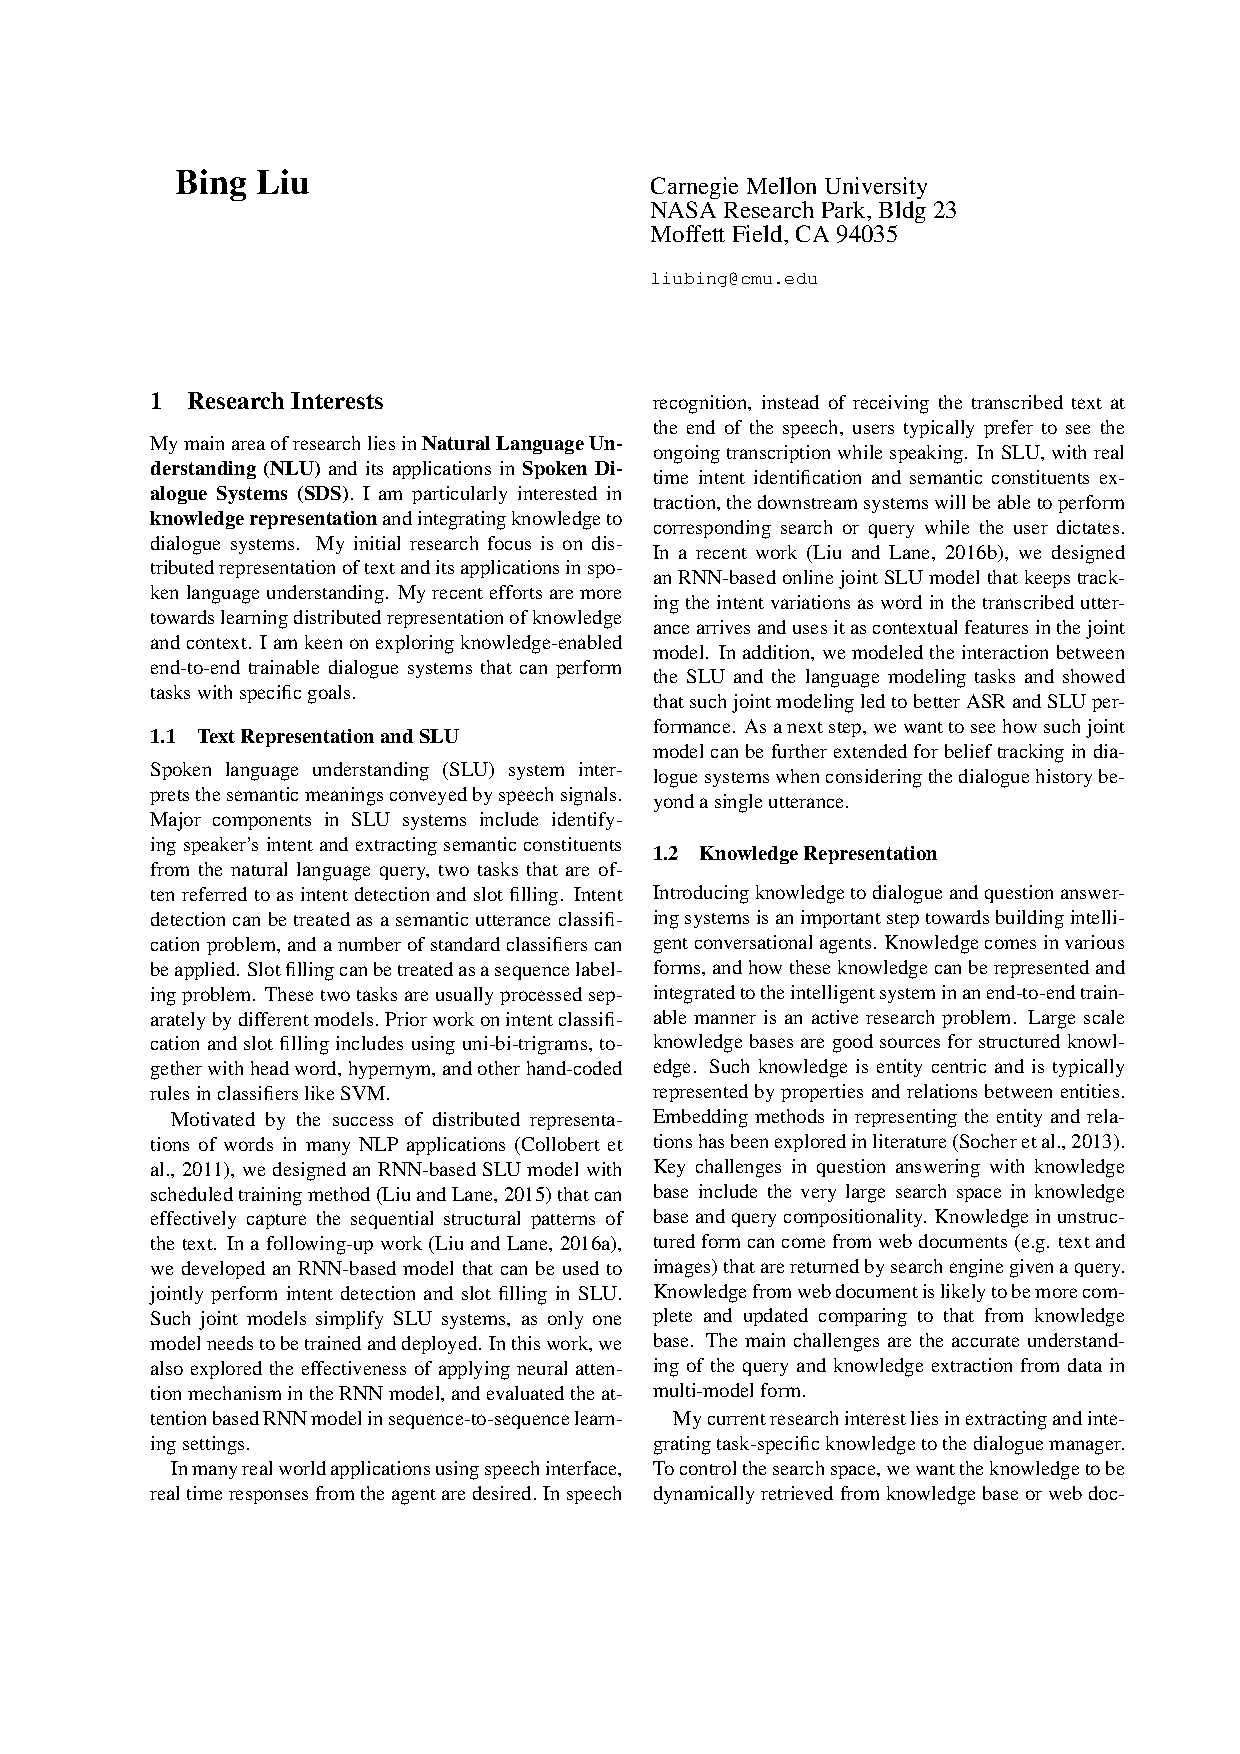
\includepdf[pages=-,pagecommand={}]{YRRSDS_2016_paper_16_bing_liu.pdf}
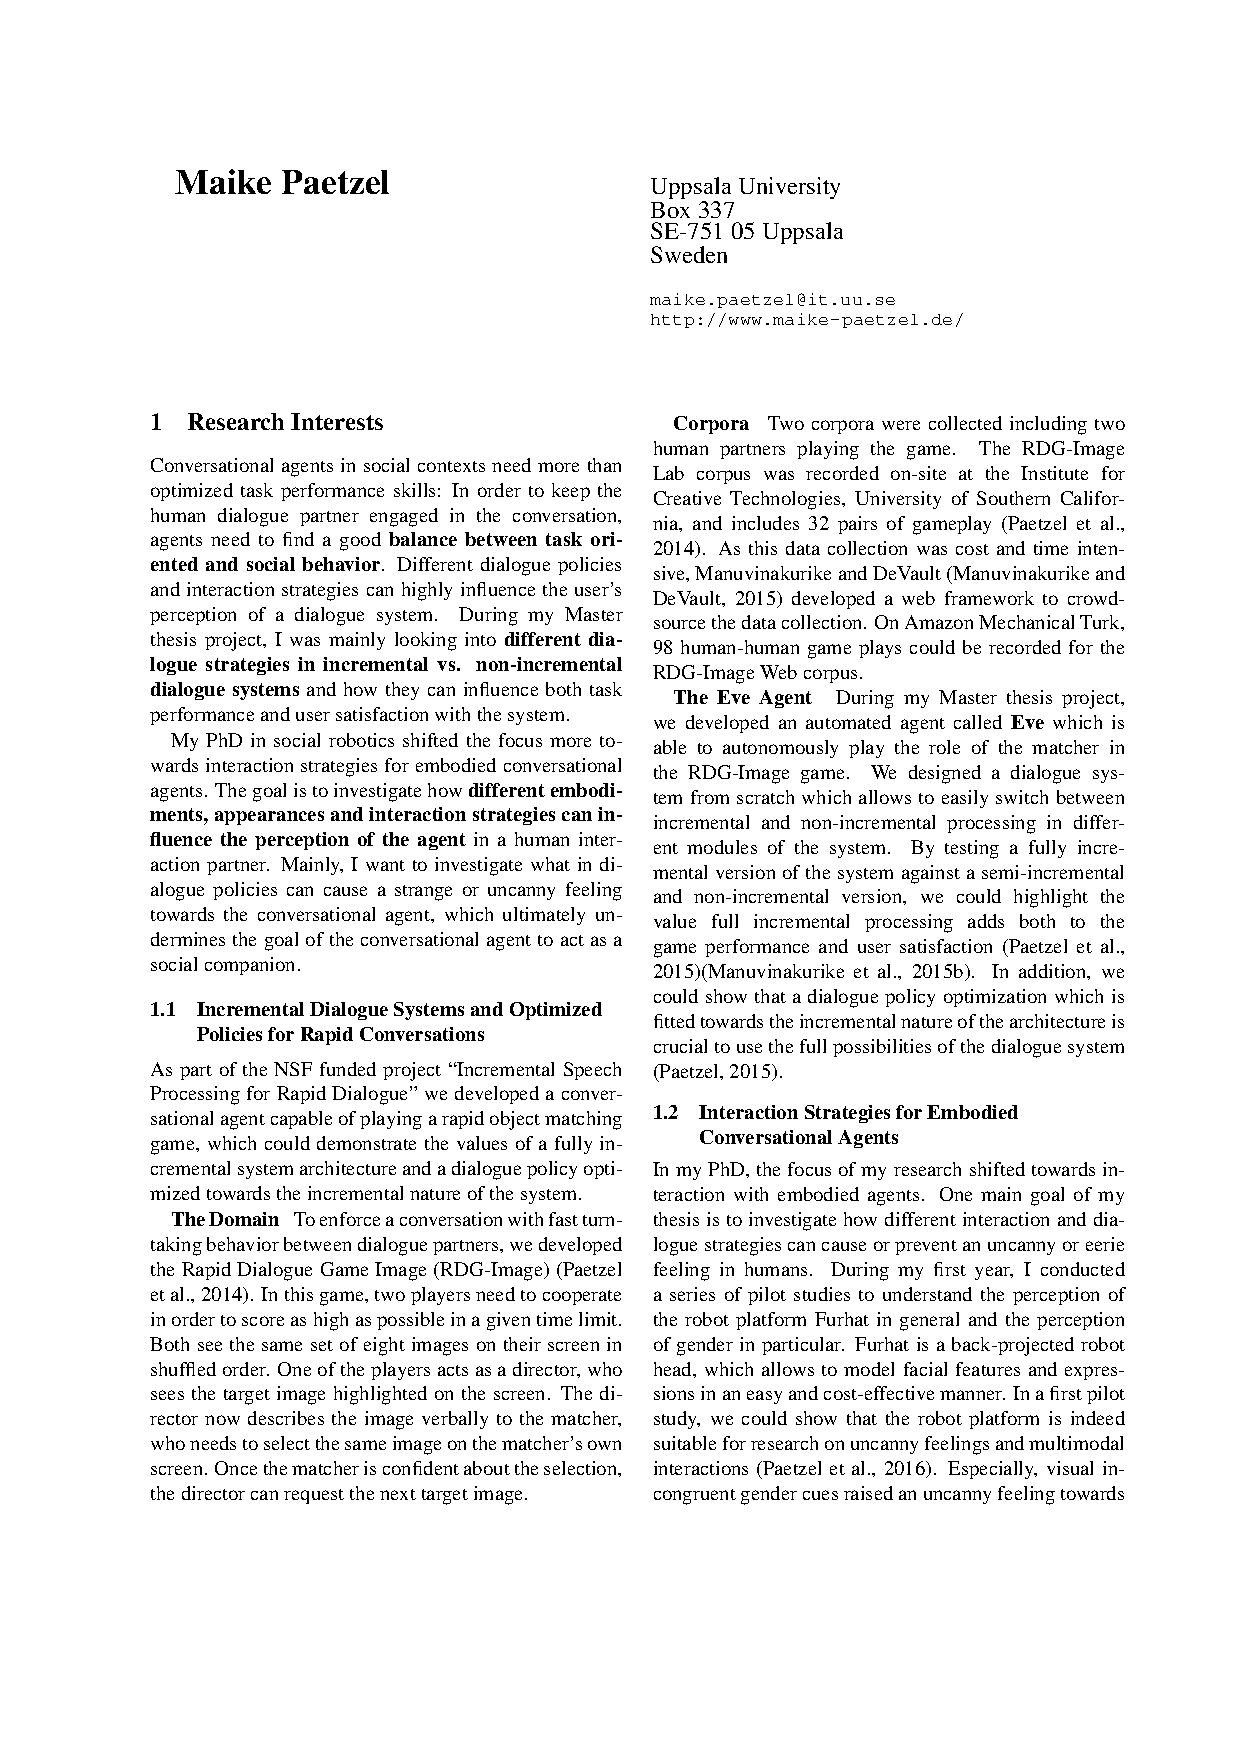
\includepdf[pages=-,pagecommand={}]{YRRSDS_2016_paper_17_maike_paetzel.pdf}
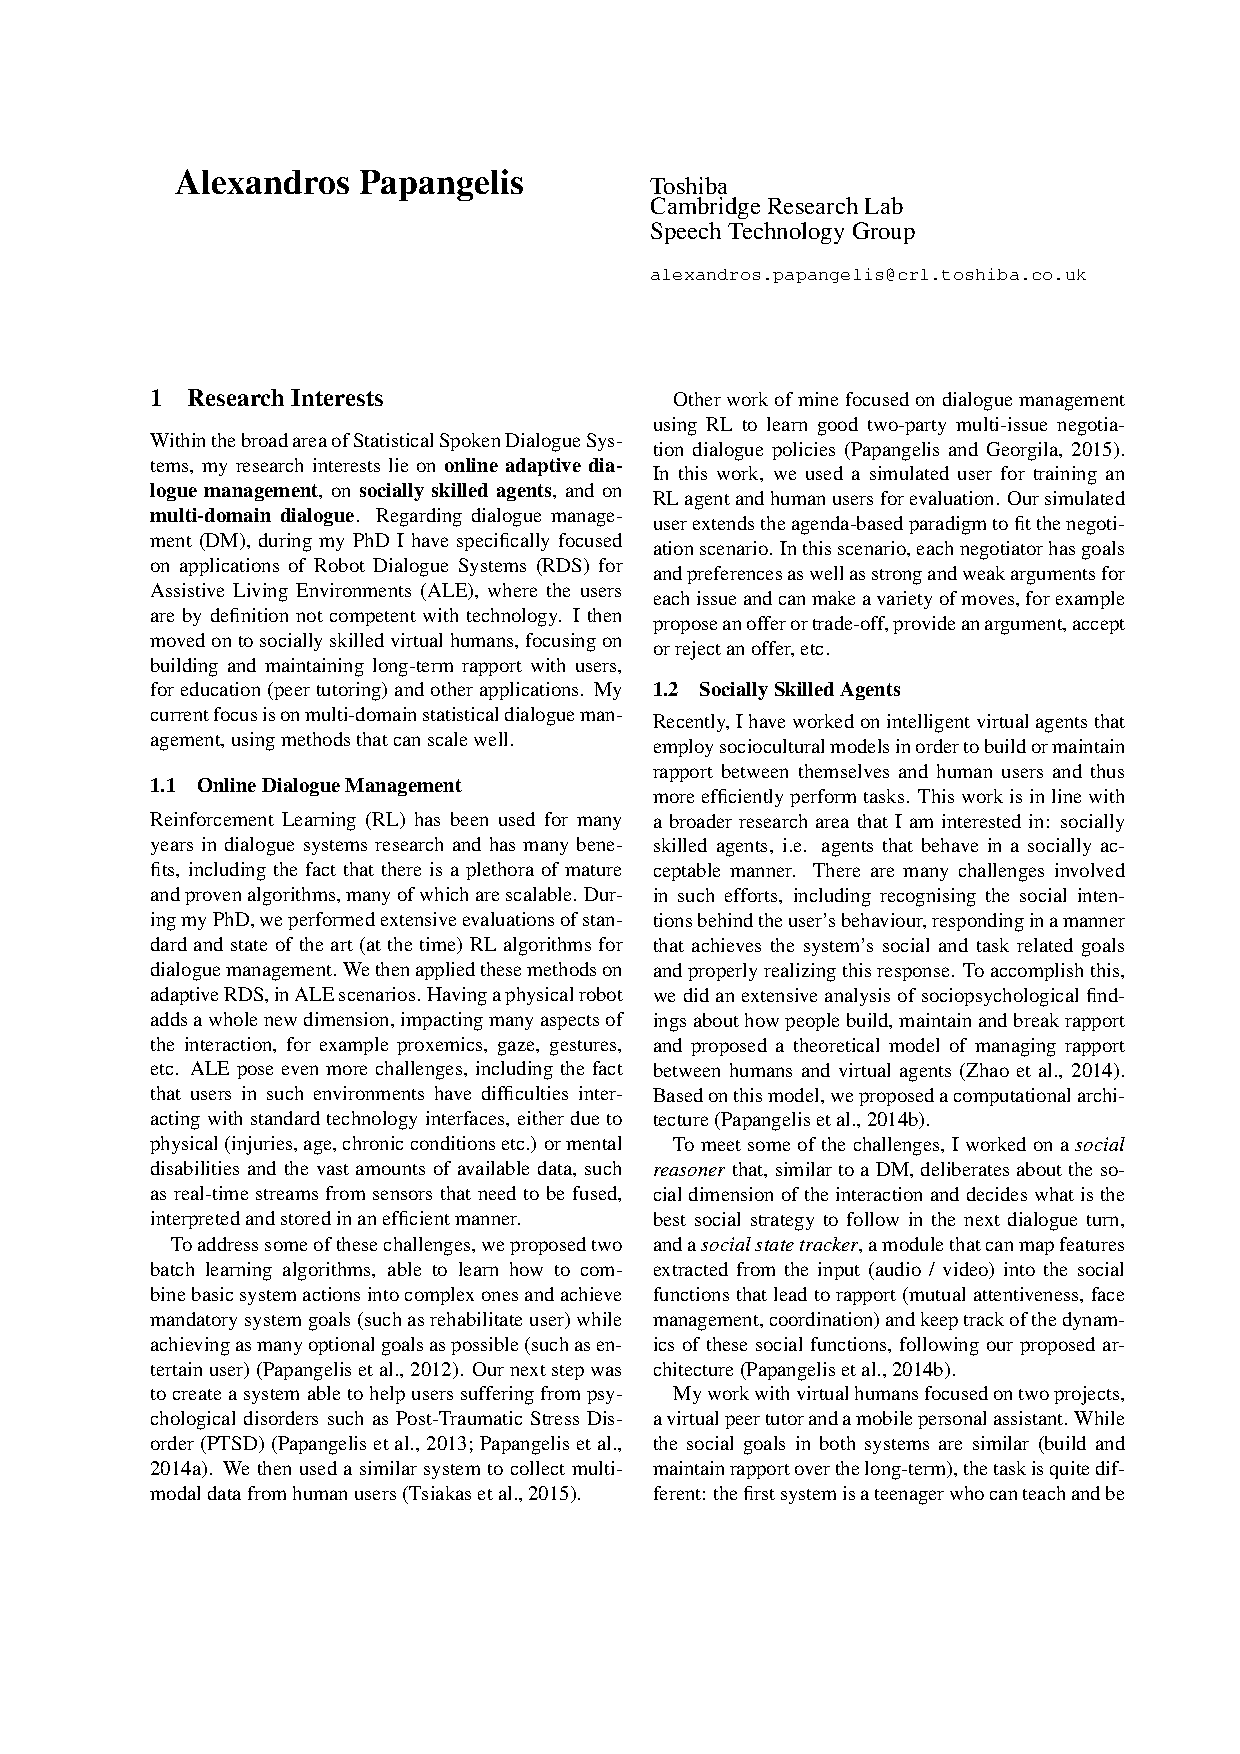
\includepdf[pages=-,pagecommand={}]{YRRSDS_2016_paper_18_alexandros_papangelis.pdf}
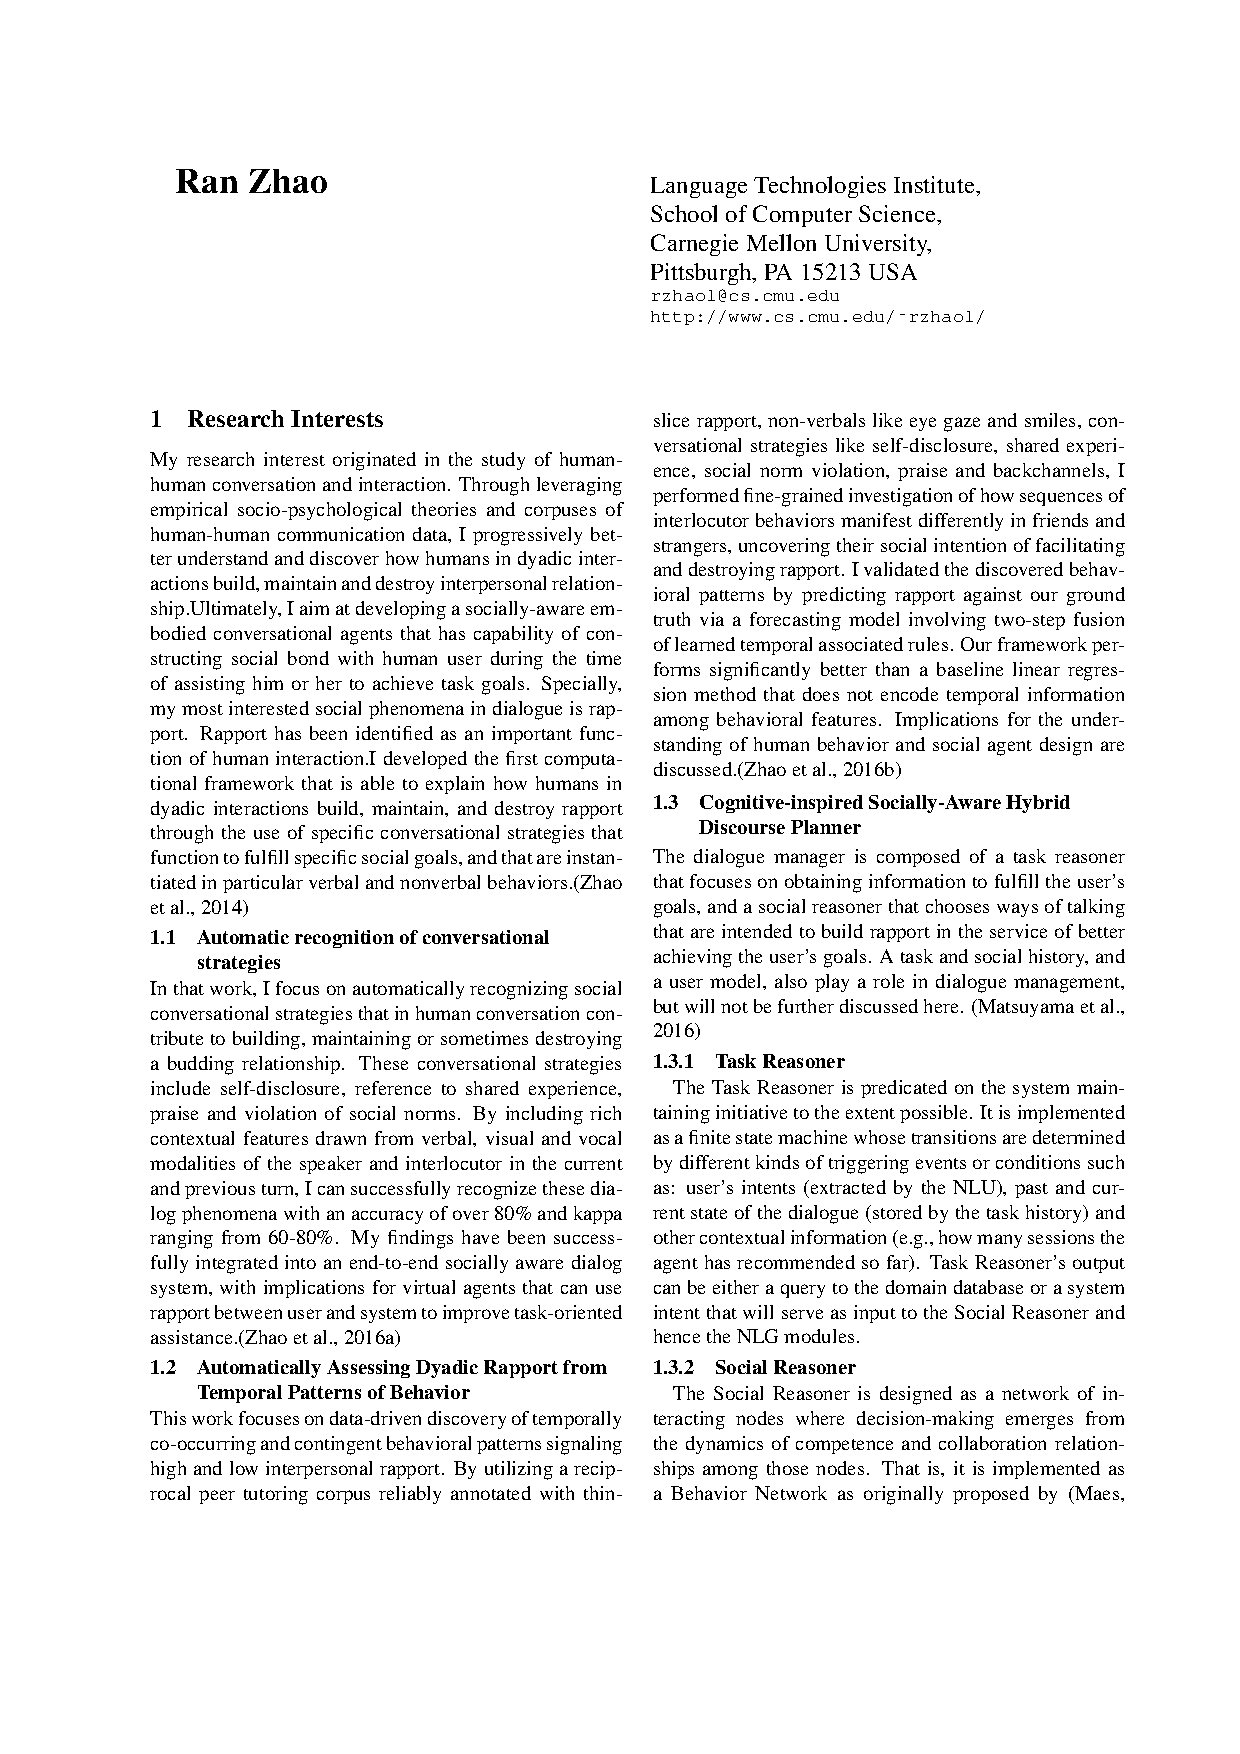
\includepdf[pages=-,pagecommand={}]{YRRSDS_2016_paper_19_ran_zhao.pdf}
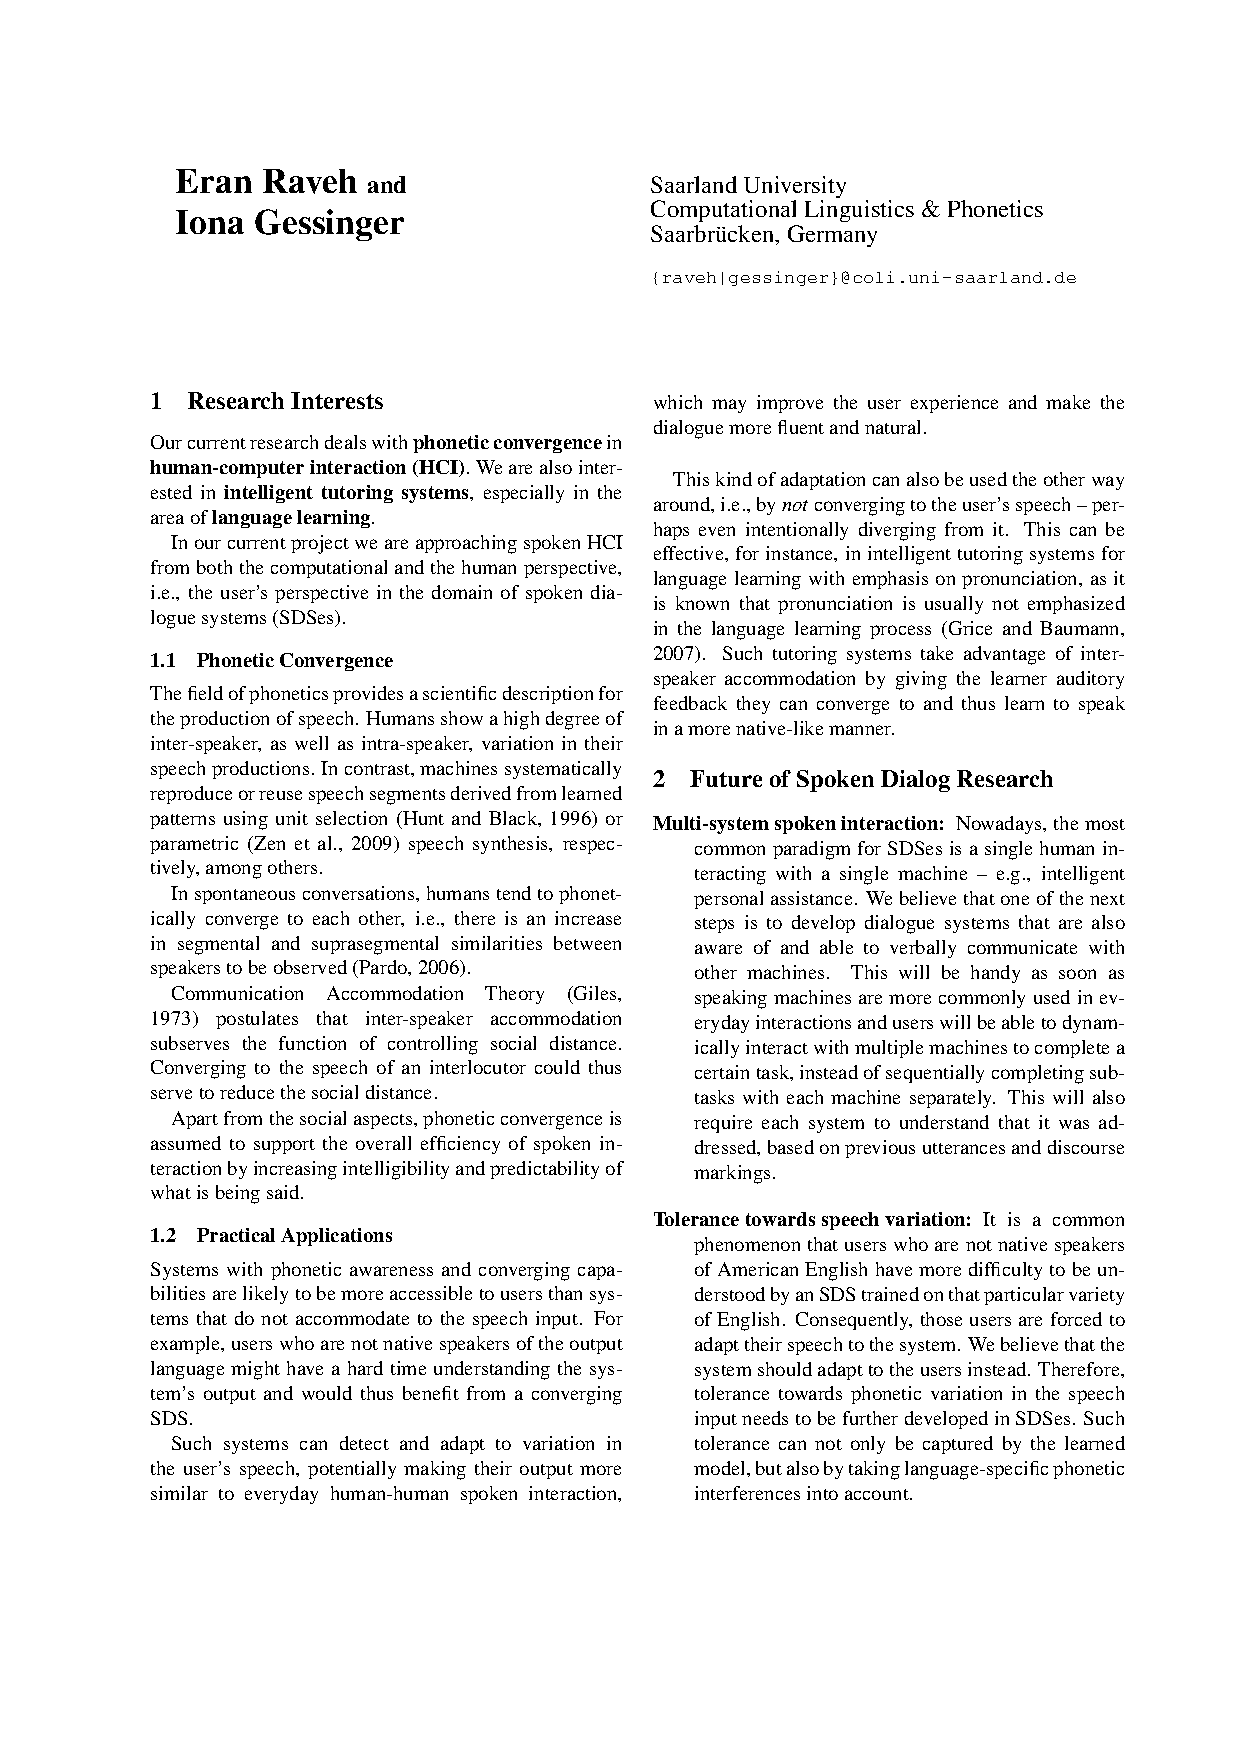
\includepdf[pages=-,pagecommand={}]{YRRSDS_2016_paper_20_eran_raveh_iona_gessinger.pdf}
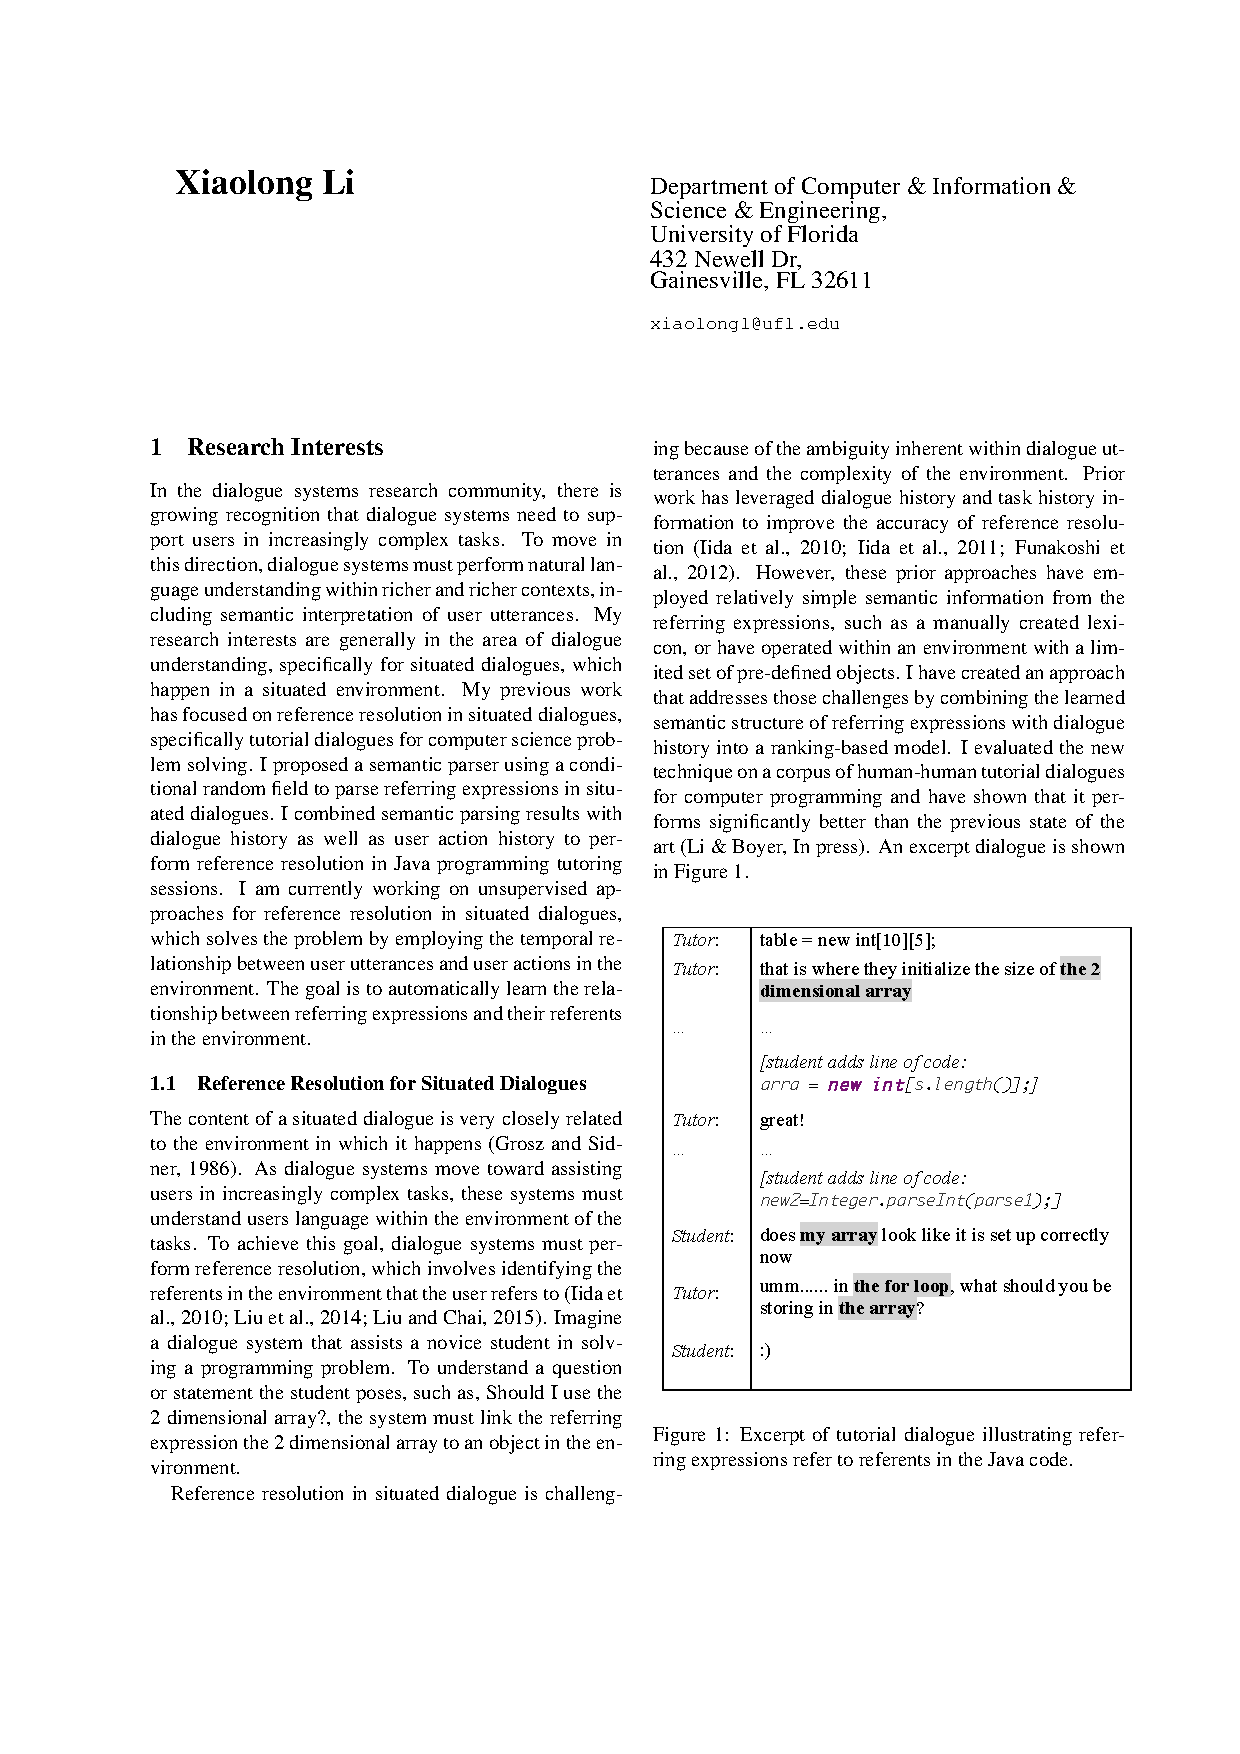
\includepdf[pages=-,pagecommand={}]{YRRSDS_2016_paper_21_xialolong_li.pdf}
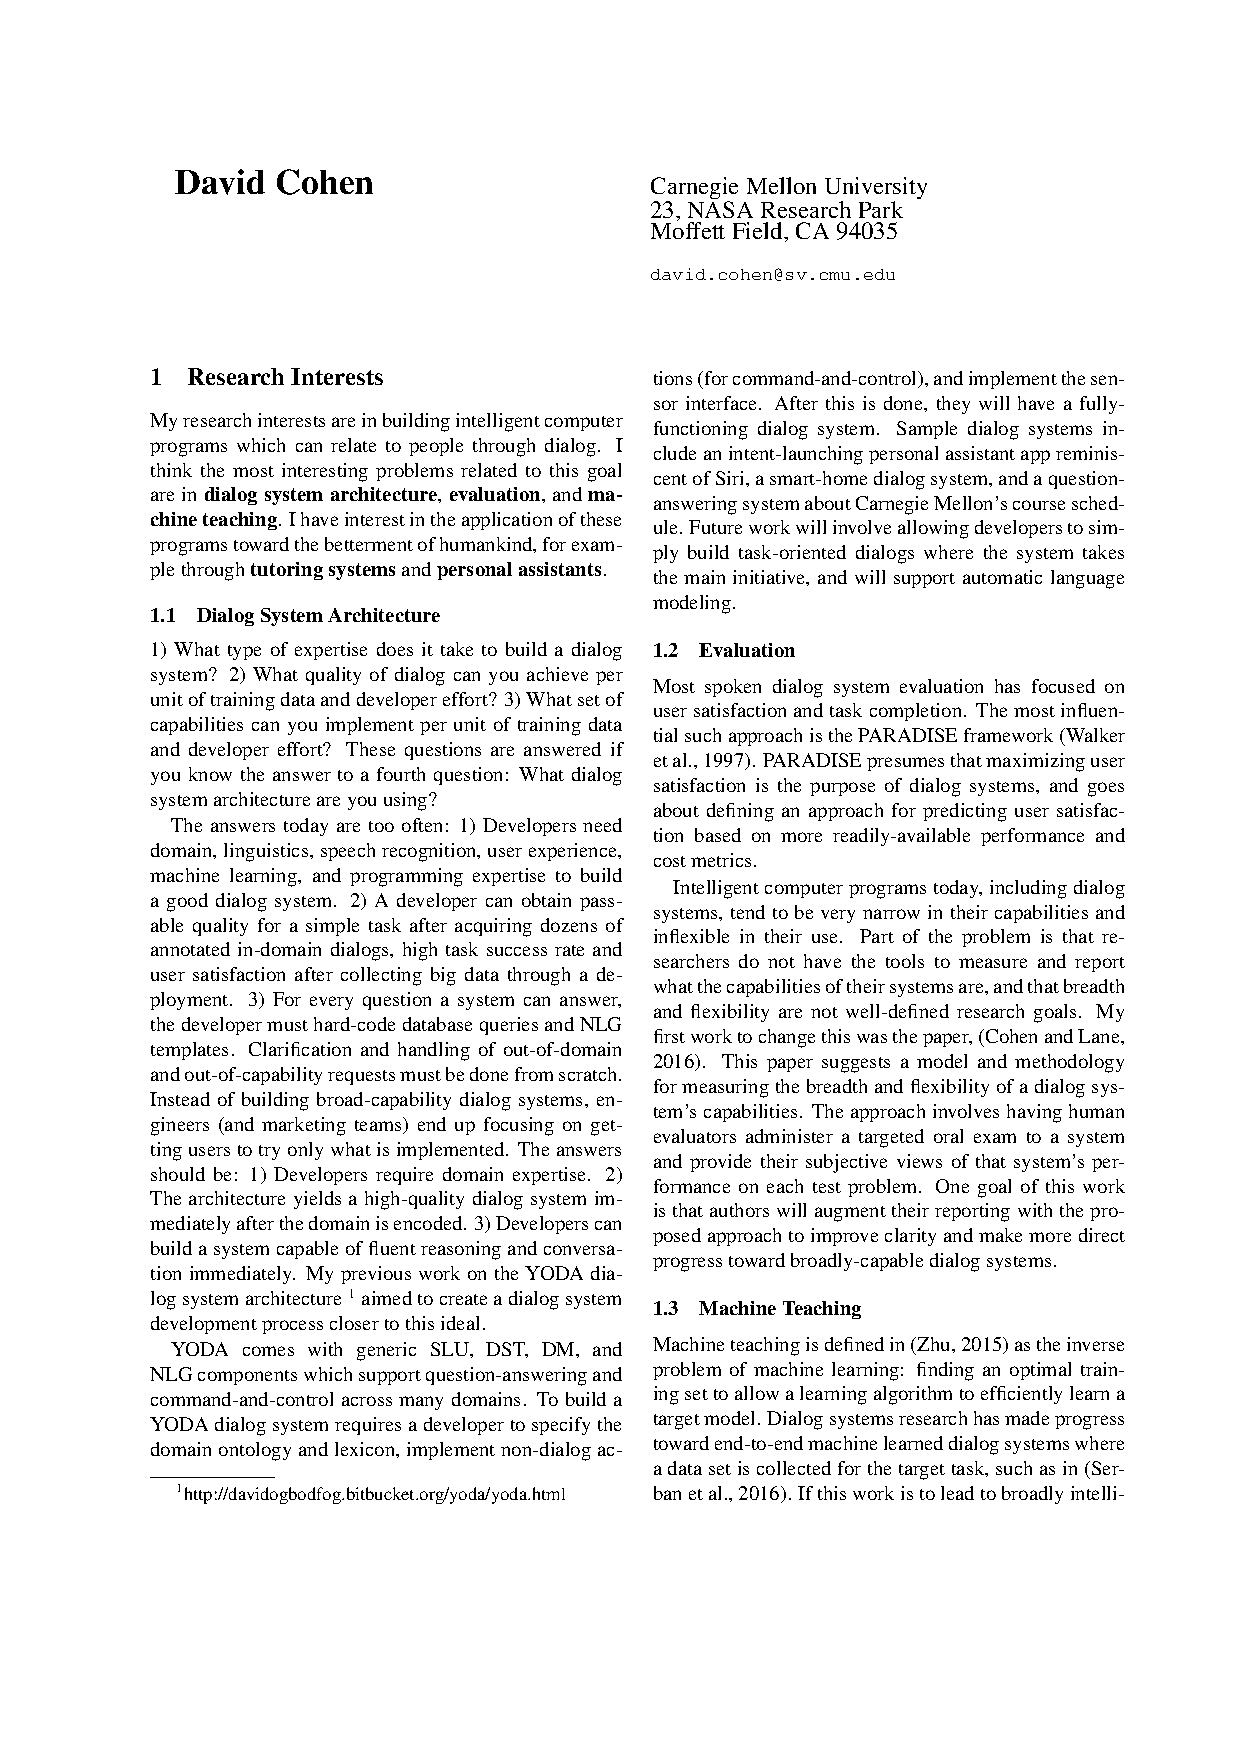
\includepdf[pages=-,pagecommand={}]{YRRSDS_2016_paper_22_david_cohen.pdf}
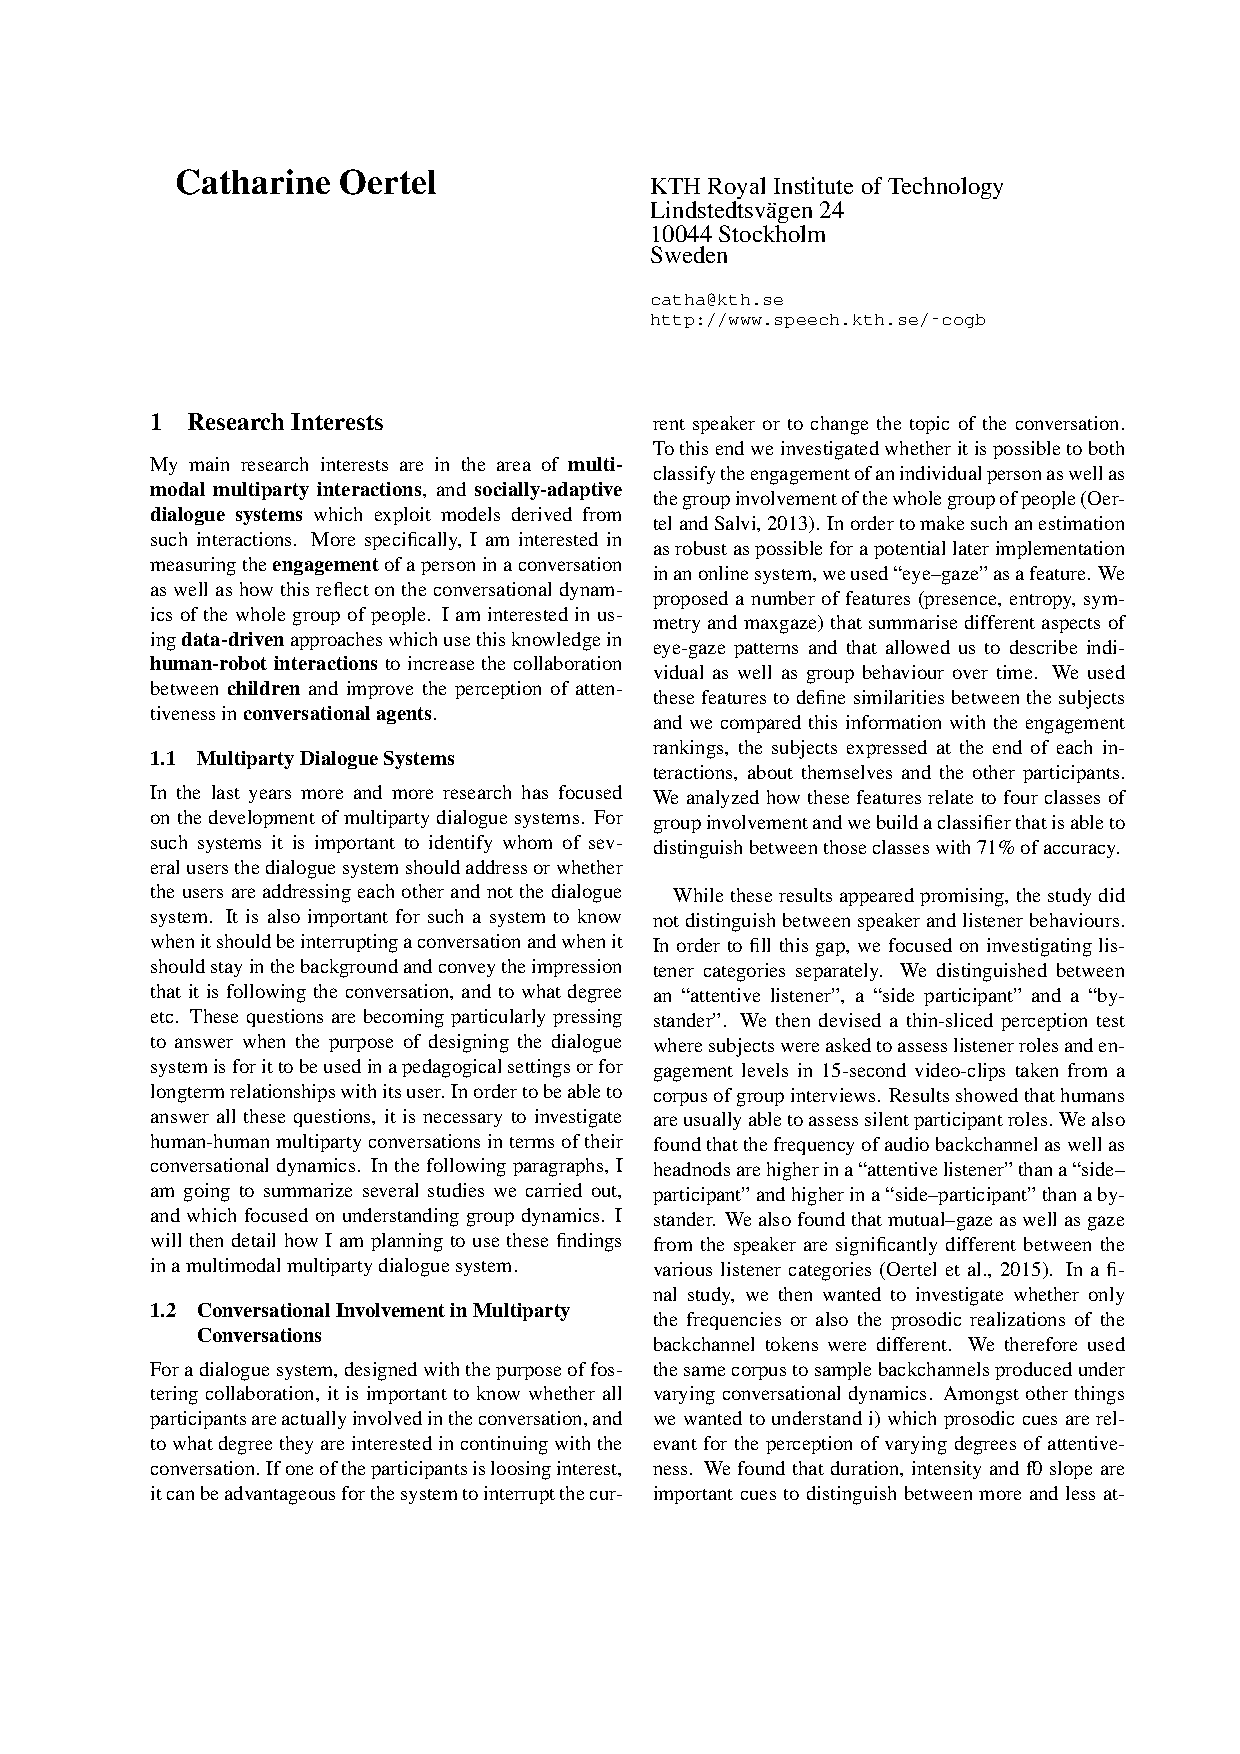
\includepdf[pages=-,pagecommand={}]{YRRSDS_2016_paper_23_catharine_oertel.pdf}
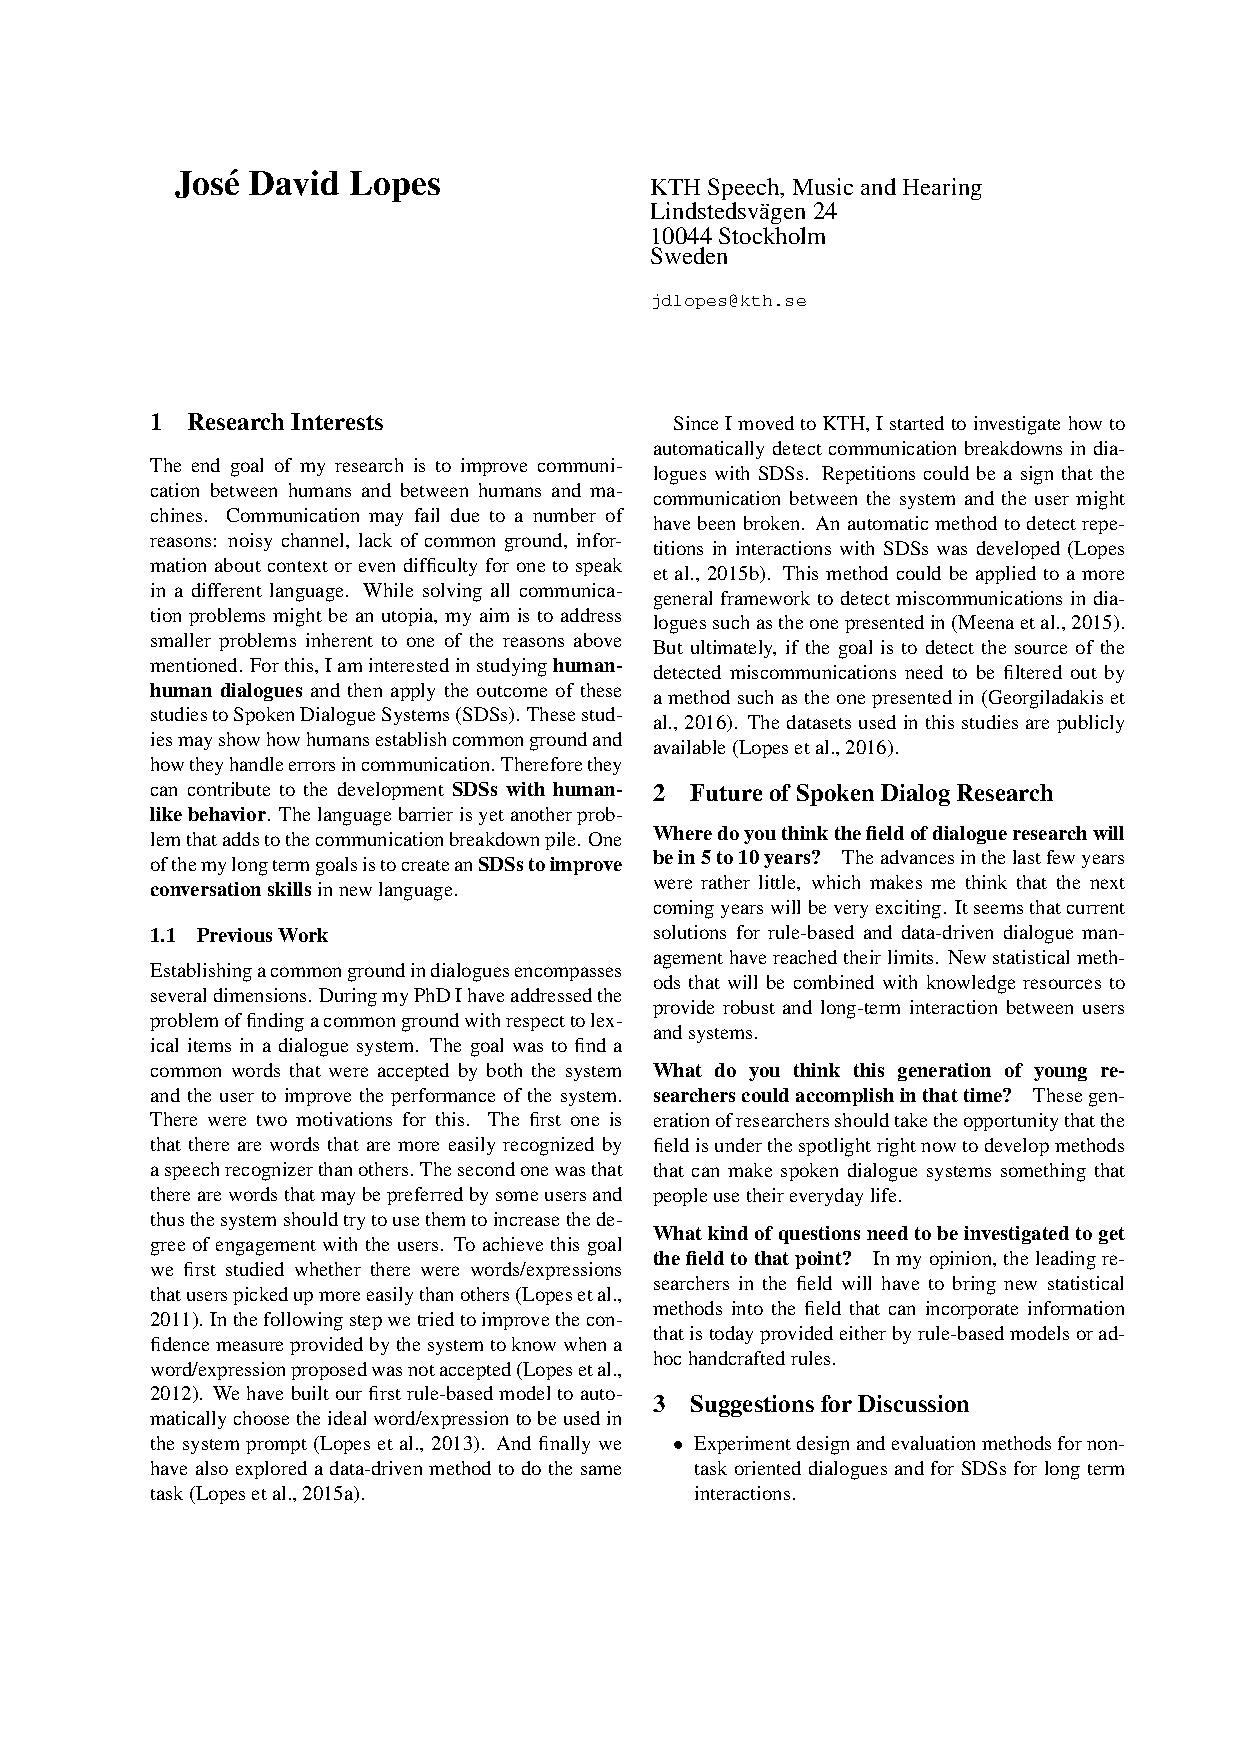
\includepdf[pages=-,pagecommand={}]{YRRSDS_2016_paper_24_jose_david_lopez.pdf}
\includepdf[pages=-,pagecommand={}]{YRRSDS_2016_paper_25_carla_gordon.pdf}
\includepdf[pages=-,pagecommand={}]{YRRSDS_2016_paper_26_eli_pincus.pdf}



\section{Closing remarks}

\end{document}
